\documentclass[10pt]{book}

% Trim, margins, heads, palette, float placement and the set-off box machinery
% all follow ~/av2atg/chygraph/book, which follows ~/av2atg/LocalNetworkGrowth.
% This book carries no mathematics, so amssymb, adjustbox and the notation
% macros are dropped. What replaces them is at the bottom: a `ledger` box for
% Parts I and II and a `design` box for Part III, both built on chygraph's
% model-box code so that the three books read as one series.
\usepackage[paperwidth=5in,paperheight=8in,includehead,
            inner=0.6625in,outer=0.2875in,top=0.56in,bottom=0.64in]{geometry}
\usepackage{graphicx}
\usepackage[round,authoryear]{natbib}
\usepackage[hidelinks]{hyperref}
\usepackage{microtype}
\usepackage{booktabs}
\usepackage{array}
\usepackage{longtable}
\usepackage{makeidx}
\makeindex

\usepackage[most]{tcolorbox}
\usepackage{tikz}
\usetikzlibrary{arrows.meta,calc,positioning,fit,backgrounds,decorations.pathreplacing}

% The index is set in one ragged-right column. The book-class default is two,
% which on a 5-inch page leaves about 1.7in of measure -- too little to break
% entries like "Comecon, terms of trade under" without overfull lines.
\makeatletter
\renewenvironment{theindex}
  {\clearpage
   \chapter*{\indexname}%
   \addcontentsline{toc}{chapter}{\indexname}%
   \markboth{\indexname}{\indexname}%
   \thispagestyle{plain}%
   \parindent\z@
   \parskip\z@ \@plus .3\p@\relax
   \raggedright
   \let\item\@idxitem}
  {\clearpage}
\makeatother

% Section headings ragged right. The class sets them justified, which on a
% 4.05in measure makes a long title overflow rather than break. Chapter heads
% are already ragged in book.cls; these two were not.
\makeatletter
\renewcommand\section{\@startsection{section}{1}{\z@}%
  {-3.5ex \@plus -1ex \@minus -.2ex}%
  {2.3ex \@plus.2ex}%
  {\raggedright\normalfont\Large\bfseries}}
\renewcommand\subsection{\@startsection{subsection}{2}{\z@}%
  {-3.25ex\@plus -1ex \@minus -.2ex}%
  {1.5ex \@plus .2ex}%
  {\raggedright\normalfont\large\bfseries}}
\makeatother

% ---------------------------------------------------------------------------
% Two set-off environments, and only two. Both are chygraph's model box with a
% different heading, so a reader coming from that book already knows that a
% shaded block is something the text has stipulated rather than derived.
%
% `ledger` is a balance: a claim and its counter-claim set down together and
% left there. Parts I and II close on one wherever the honest answer is that
% both things are true at once, which on this subject is most of the time. A
% ledger is not a summary of the section above it -- if the two say the same
% thing, one of them is redundant.
%
% `design` is a numbered institutional rule for Part III, stated as a rule and
% never as a paragraph the reader has to parse back into one. Its interior is
% the `rules` list below, so that a design can be argued with one clause at a
% time. A design box is always a proposal and never a description of anything
% that exists.
% ---------------------------------------------------------------------------
% BREAKABLE. The first implementation of these boxes was chygraph's model box,
% an lrbox inside a minipage. That cannot break across a page, so a box longer
% than the text height runs off the bottom of the page silently -- which is what
% Design 14.2 did, by 88pt. Several of Part III's design boxes are longer than a
% page and always will be, so the box has to break. tcolorbox with breakable is
% the same choice Local network growth makes for its calculation box.
%
% The counter is kept as a plain LaTeX counter rather than tcolorbox's auto
% counter, and stepped BEFORE the box opens, so that a \label placed just inside
% \begin{design} still resolves against \thedesign -- which is how every
% cross-reference in Part III is written.
\newcounter{design}[chapter]
\renewcommand{\thedesign}{\thechapter.\arabic{design}}
\newenvironment{design}[1]
  {\par\addvspace{\medskipamount}%
   \refstepcounter{design}%
   \begin{tcolorbox}[breakable,enhanced,colback=black!7,colframe=black!7,
     boxrule=0pt,arc=0pt,outer arc=0pt,
     left=6pt,right=6pt,top=6pt,bottom=6pt,
     fontupper=\small]%
   \noindent{\normalsize\textbf{Design \thedesign.\ #1}}\par\nobreak\smallskip}
  {\end{tcolorbox}\addvspace{\medskipamount}\noindent\ignorespacesafterend}

\newenvironment{ledger}[1]
  {\par\addvspace{\medskipamount}%
   \begin{tcolorbox}[breakable,enhanced,colback=black!7,colframe=black!7,
     boxrule=0pt,arc=0pt,outer arc=0pt,
     left=6pt,right=6pt,top=6pt,bottom=6pt,
     fontupper=\small]%
   \noindent{\normalsize\textbf{The ledger: #1}}\par\nobreak\smallskip}
  {\end{tcolorbox}\addvspace{\medskipamount}\noindent\ignorespacesafterend}

% The clause list inside a design box: tight, hanging-indented, with the clause
% name carried by \rl so that renaming the convention is a one-line edit here.
\newenvironment{rules}
  {\begin{list}{}{%
     \setlength{\leftmargin}{1.5em}\setlength{\itemindent}{-1.5em}%
     \setlength{\labelwidth}{0pt}\setlength{\labelsep}{0pt}%
     \setlength{\topsep}{0pt}\setlength{\parsep}{0pt}%
     \setlength{\itemsep}{3pt plus 1pt}\setlength{\listparindent}{0pt}}}
  {\end{list}}
% The 1.5em slot is the list's hanging indent, so continuation lines line up
% under the clause name. Labels must fit it: number the clauses, as every
% design box in this book does.
\newcommand{\rl}[2]{\item[]\makebox[1.5em][l]{(#1)}\textsc{#2}\hspace{0.4em}}


% Compact running heads that fit the narrow 5x8 page.
\usepackage{fancyhdr}
\pagestyle{fancy}
\fancyhf{}
\fancyhead[LE,RO]{\small\thepage}
\fancyhead[RE]{\small\nouppercase{\leftmark}}
\fancyhead[LO]{\small\nouppercase{\rightmark}}
\renewcommand{\headrulewidth}{0.3pt}
\fancypagestyle{plain}{\fancyhf{}\renewcommand{\headrulewidth}{0pt}\fancyfoot[C]{\small\thepage}}

% Make the blank verso pages inserted before each chapter truly blank.
\makeatletter
\def\cleardoublepage{\clearpage\if@twoside\ifodd\c@page\else
  \hbox{}\thispagestyle{empty}\newpage\if@twocolumn\hbox{}\newpage\fi\fi\fi}
\makeatother

% Grayscale palette (the book is printed in black and white).
\colorlet{accent}{black!80}
\colorlet{accentB}{black!50}

% Looser float placement so figures do not leave near-empty pages on the small trim.
\renewcommand{\topfraction}{0.9}
\renewcommand{\bottomfraction}{0.8}
\renewcommand{\textfraction}{0.07}
\renewcommand{\floatpagefraction}{0.7}
\setcounter{topnumber}{2}
\setcounter{totalnumber}{3}

\newcolumntype{L}[1]{>{\raggedright\arraybackslash}p{#1}}

% A figure asserted from a secondary source and not yet traced to a primary one
% carries \unv. Every occurrence is listed in verify.md. The macro prints
% nothing, so the mark is a working device and not a mark on the page.
\newcommand{\unv}{}

\hyphenation{cuen-ta-pro-pis-mo cuen-ta-pro-pis-tas Bio-Cuba-Farma
  bio-tech-nol-o-gy des-a-bas-te-ci-mien-to par-a-me-tra-cion}

\begin{document}

% Roman front matter, so the preface and the note on sources have page numbers
% and appear in the contents with them. Arabic numbering restarts at
% \mainmatter, below.
\frontmatter

\title{A prospect of Cuba: Past and Future}
\author{Alexei Vazquez}
% Empty rather than absent: \maketitle would otherwise stamp the build date on
% the title page and change it silently on every run.
\date{}
\maketitle

\thispagestyle{empty}
\vspace*{\fill}
\begin{center}
{\itshape For those who stayed, and those who left.}
\end{center}
\vspace*{\fill}
\clearpage

\chapter*{Preface}
\addcontentsline{toc}{chapter}{Preface}
\markboth{Preface}{Preface}

Cuba is one of the few countries about which almost nobody writes carefully.
The literature divides into two libraries that do not read each other. One
records a small poor island that abolished illiteracy, built a health system
that outperformed its income by a wide margin, sent doctors to forty countries,
and did it under six decades of economic siege by the largest economy on earth.
The other records a one-party state that jailed its poets, criminalised its
markets, drove a fifth of its people into exile, and ended the period with a
grid that could not keep the lights on. Both libraries are accurate. Neither is
honest, because each is complete only by omission.

This book tries to hold both at once, and it does so for a practical reason
rather than a scholarly one. The last part of the book is a design: a proposed
socio-political and economic system for Cuba from 2026 forward. A design is
only as good as its account of the initial conditions. If you believe the first
library, you will design as though the only thing wrong is the embargo, and you
will produce a plan that fails the moment it meets a Cuban who wants to open a
shop. If you believe the second, you will design as though the only thing
wrong is socialism, and you will produce a plan that dismantles a public health
system it cannot replace, hands the assets to whoever is standing closest, and
reproduces in ten years the inequality that made 1959 possible. Both failures
have been run as experiments elsewhere. Neither needs a second trial.

So Parts I and II are not throat-clearing. They are the constraint set. Part I
covers 1959 to 1990, the years in which Cuba built its social state and paid
for it with a Soviet subsidy and a closed politics. Part II covers 1990 to
2026, the long adjustment to the loss of that subsidy: two full cycles of
liberalise-under-duress and recentralise-when-the-pressure-lifts, ending in the
worst material crisis the revolution has faced, worse in some dimensions than
the Special Period, and the largest emigration in Cuban history. Part III asks
what can be built on what is left.

What is left is more than the ruin makes it look. Cuba has a population that
can read, calculate and be trained quickly; a medical and biotechnological
establishment with real products and a reputation that is still worth money;
some of the best beaches, reefs and colonial cities in the hemisphere,
underexploited; eleven hundred kilowatt-hours of sunlight per square metre per
year falling on a country that currently burns imported fuel oil; a diaspora of
roughly two million people, many of them wealthy, most of them one flight from
home; and, unusually for a poor country, low violent crime and a functioning
public order. Those are the assets. The book's argument is that they compose:
that education plus connectivity plus a residence regime for mobile knowledge
workers is a second export track alongside tourism, that solar plus storage
converts the country's largest recurring hard-currency cost into a domestic
one, and that biotechnology is the one sector where Cuba already holds
something the world will pay for and has never been organised to sell.

The book's argument is also that none of it works without the boring part.
Every asset listed above has been available for twenty years and has not been
converted, and the reason is not the embargo alone. It is that Cuba lacks the
institutional machinery that turns an asset into an investment: enforceable
contracts, a currency that means something, a customs service that does not
take a cut, a court a foreigner can lose in fairly, a procurement system that
publishes what it bought. A country can have sunshine and doctors and beaches
and still be poor, and Cuba is the proof. So the longest chapters in Part III
are not the ones about solar panels. They are the ones about money,
about property, and about corruption, which is the failure mode every
transition of this type has actually died of.

One commitment in Part III is not up for argument in this book, and it should
be stated at the front rather than arrived at in the middle. The design keeps a
universal welfare state at Western European standard --- health, education,
pensions, disability, income support --- and everything else in Part III is
arranged around being able to afford it. This is not sentiment about the
revolution. It is the reading of the record in Parts I and II: the social state
is the one asset those sixty-seven years produced that is unambiguously worth
keeping, it is the thing that protects the Cubans most exposed if a transition
goes badly, and it is also an economic input rather than only a transfer, since
the education system is precisely what the second track and the biotechnology
sector are built out of.

What changes is not the benefit but who pays for it. Cuba's welfare state has
never been financed by Cubans. It was financed by Soviet terms of trade until
1990, by Venezuelan oil in the 2000s, and in the intervals by printing money
and by not maintaining anything, which is why it has come close to collapse
twice in living memory. An entitlement funded by an external rent lasts exactly
as long as the rent. The European systems this book takes as its standard are
financed by taxing a domestic base, which is why they survive changes of
government, of commodity price and of patron. So the proposal is a European
benefit structure on a European tax structure --- a broad-based, simply
administered tax system of a kind Cuba has never had --- and the cost of that
commitment, a tax burden well above the Latin American norm, is stated in the
chapters rather than hidden in them. A country that wants Nordic outcomes has
to collect Nordic revenue, and there is no version of this in which the
arithmetic is pleasant.

I write as a Cuban of the diaspora and a physicist by training, which shapes
the book in two ways worth declaring. It is why Part III is written as a set of
numbered institutional rules rather than as an essay: a design that cannot be
stated as rules is not a design, and rules can be argued with one at a time. It
is also why the book is not neutral about outcomes even where it tries to be
neutral about facts. It wants Cuba to be prosperous, open and its own. It does
not assume those three are automatically compatible, and where they conflict,
the text says so instead of choosing quietly.

Nothing here is a prediction. The prospect of the title is the older sense of
the word: a view of what lies ahead from where one is standing, drawn to scale.

\chapter*{A note on sources and numbers}
\addcontentsline{toc}{chapter}{A note on sources and numbers}
\markboth{A note on sources}{A note on sources}

Cuban statistics are a problem with three layers, and a book that quotes them
without saying so is misleading its reader by arithmetic rather than by
argument.

The first layer is ordinary. Cuba's national statistics office, the Oficina
Nacional de Estad\'istica e Informaci\'on (ONEI), publishes an annual
\emph{Anuario Estad\'istico} that is detailed, internally consistent, and by
the standards of the region reasonably competent. Health and education series
in particular are collected by an administrative apparatus that reaches every
municipality, and the vital-registration coverage is close to complete, which
is more than can be said for most countries at Cuba's income level. Where this
book quotes life expectancy, infant mortality, school enrolment or physician
counts, ONEI is usually the source and the figure is usually trustworthy in the
narrow sense that the state measured what it says it measured.

The second layer is the exchange rate, and it corrupts everything monetary. For
most of the period covered here the Cuban state carried an official rate of one
peso to one dollar for enterprise accounting while households changed money at
twenty-four or twenty-five, and after 2021 at rates that in the informal market
passed three hundred. Any figure denominated in Cuban pesos and converted at an
official rate --- GDP, GDP per capita, wages, the value of the social wage, the
cost of a subsidy --- is therefore not a measurement but an accounting
convention, and cross-country comparisons built on it are close to meaningless.
Cuba's reported GDP per capita has for decades placed it in the upper-middle
band of Latin America while its consumption basket has looked like the lower.
Both facts are real; the contradiction is in the conversion. This book gives
peso figures with the rate attached, prefers physical quantities to monetary
ones wherever a physical quantity exists --- tons of sugar, barrels of oil,
megawatts, doctors per thousand, calories per day --- and treats any single
figure for Cuban GDP as an argument rather than a datum.

The third layer is political, and it runs in both directions. The state does
not publish, or publishes late and partially, series that embarrass it: the
scale of the 1993--94 contraction was reconstructed years afterwards, the
prison population is not disclosed, the count of political detentions is
produced by opposition monitors and by no one else, and after 2020 several
routine series in the \emph{Anuario} simply stopped appearing. Against this,
the exile literature has its own inflations, some of them very large and very
durable --- the twenty thousand dead attributed to Batista's last years, a
figure that originated in a newspaper and has never been supported by anything
resembling a count, is the best-known example, and it is repeated to this day
by people who would never accept a Cuban government figure on the same
evidence. Where a contested number appears in this book it appears as a range
with the disagreement named, and where the honest answer is that nobody knows,
the text says nobody knows.

Three practical conventions follow.

Figures asserted from a secondary source that has not been traced to a primary
one are marked in the manuscript and listed in \texttt{verify.md} in the book's
source directory. The mark prints nothing, so it does not clutter the page; it
exists so that the list of unverified claims is mechanically extractable rather
than a matter of memory.

Where a range is given, the endpoints are the two most defensible published
estimates and not the extremes of what has been claimed. A figure that has been
claimed only by a party with an interest in it, and never independently, is
described that way rather than averaged into a range as though it were
evidence.

Where the book states a causal claim --- that the embargo cost Cuba this much,
that the 2021 monetary reform caused that much inflation --- it states what
would have to be true for the claim to hold, because on this subject almost
every causal claim is contested by someone whose objection is not frivolous.
The two standing questions, how much of Cuba's poverty is the embargo and how
much is the model, and how much of Cuba's social achievement is socialism and
how much is what any determined state can buy with a large enough external
subsidy, are not settled in this book. They are, however, kept visible, because
Part III's design has to work under either answer.


% The contents lists parts and chapters only: with twenty-three chapters,
% breaking it down to sections runs to eight pages and helps nobody.
\setcounter{tocdepth}{0}
\tableofcontents

\mainmatter

% ===========================================================================
\part{1959--1990}
% The Soviet-era republic, from the inheritance it took over to the year the
% subsidy stopped. Five chapters, chronological, each carrying both sides of
% its own ledger rather than deferring the bad news to a later chapter.
% ===========================================================================

\chapter{The inheritance}
\label{ch:inheritance}

\section{A country that was not poor, and was not developed}

On the last day of 1958 Cuba had about 6.6 million people, a fifth of the
population of Spain on an island slightly larger than Portugal, and it was by
most aggregate measures one of the four or five richest countries in Latin
America.\unv{} It had more television sets per head than any country in the
region and among the highest counts in the world; it had one of the densest
railway networks in the hemisphere, inherited from sugar; it had roughly one
physician for every thousand inhabitants, a ratio comparable with much of
Western Europe at the time; it had a literate majority, 76 per cent of the
population over ten by the 1953 census; and it had a life expectancy at birth
somewhere around 62 years \citep{perezjr2015}, higher than every mainland Latin American country
except Argentina and Uruguay.\unv{}

Every one of those numbers is a national average, and every one of them is
concealing the thing that actually mattered, which is that Cuba in 1958 was not
one country but two economies bolted together at the port of Havana.

The urban economy, and above all the capital, was genuinely modern. Havana had
department stores, an air-conditioned bus system, a stock exchange, medical
specialists, a professional press of a dozen daily papers, a university with a
real research tradition, and a middle class of professionals, shopkeepers and
unionised industrial workers whose standard of living would not have been out
of place in southern Europe. Cuban organised labour was strong --- the sugar and
transport unions in particular --- and had extracted job protections and wage
floors that were unusual in the region and that would, a decade later, become
one of the constraints the revolution had to negotiate with rather than around.

The rural economy was something else. The most-quoted single source on it is a
survey of a thousand rural wage-worker families conducted in 1956--57 by the
Agrupaci\'on Cat\'olica Universitaria, a lay Catholic organisation with no
sympathy for what came after, which is why the figures survived scrutiny. It
found that among rural workers 4 per cent ate meat with any regularity, 1 per
cent ate fish, 11 per cent drank milk; that 43 per cent could not read; that
about 60 per cent lived in dwellings with earth floors and thatch roofs; that
under 10 per cent had electricity and about 2 per cent running water \citep{perezstable2012}; and that
the median family's annual income was a fraction of the urban wage.\unv{} The
survey was published in a Catholic magazine in 1957 and its findings were not
seriously contested at the time. Approximately 43 per cent of Cubans lived in
the countryside.

So the honest description of pre-revolutionary Cuba is neither the plundered
colony of the official histories nor the prosperous republic of the exile
memoirs. It is a middle-income country with a first-world capital, a
third-world interior, and a distribution so wide that the national average
describes almost nobody.

\section{Sugar, and the shape it gave everything}

The reason the two economies existed is sugar, and the reason sugar dominated
is a policy instrument in Washington called the quota.

Sugar was roughly four-fifths of Cuban export earnings and had been for
half a century.\unv{} Under the reciprocal trade arrangements that governed
Cuban--American commerce, the United States bought a guaranteed tonnage at a
price above the world market and in return Cuban tariffs favoured American
manufactures. The arrangement was, in the short run, extremely good for Cuba:
it converted a volatile commodity into a stable annuity and it underwrote the
consumption of the urban middle class. In the long run it did three things that
compounded.

It suppressed industry. Why build a Cuban shoe factory when the tariff schedule
made American shoes cheap and the quota made sugar dollars certain? Cuban
manufacturing outside sugar processing, tobacco and a handful of consumer goods
was thin, and what existed was largely assembly.

It froze the land. Sugar wants large flat holdings and cheap seasonal labour,
and it got both. By the 1946 agricultural census something like 8 per cent of
farms held about 70 per cent of the farmland, and a substantial share of the
cane land --- the standard estimates run from a quarter to two-fifths of milling
capacity --- was owned by American companies.\unv{} Much of the best land was
held out of production entirely as a reserve against a good year, in a country
that imported a third of its food.

And it made unemployment structural. The cane harvest, the \emph{zafra}, ran
roughly January to May. The rest of the year was the \emph{tiempo muerto}, the
dead season, in which several hundred thousand cane workers had no work at all.
Annual average unemployment in the mid-1950s ran around 16 per cent and the
seasonal swing was far wider than that.\unv{} A country cannot build a stable
politics on an economy that lays off a fifth of its workforce every June.

To this was added the ownership question, which mattered less economically than
it did politically. American capital owned most of the electric and telephone
utilities, most of the nickel, a large share of the banking and the refineries,
and the milling capacity noted above. Whether this was extraction or investment
is a genuinely arguable question --- the utilities were real utilities and the
mills were real mills. What is not arguable is that it made the commanding
heights of the Cuban economy answerable to decisions taken in another country,
and that this was intolerable to a generation of Cubans who had grown up on the
nationalism of the 1933 revolution and the constitution of 1940.

\section{The republic that could not hold}

Cuba's 1940 constitution was, on paper, among the most advanced documents of
its era anywhere: it guaranteed the eight-hour day, paid holidays, the right to
strike, equal pay for women, free compulsory education, and it prohibited
latifundia and set limits on foreign landholding. Very little of the social
programme was ever implemented by enabling legislation, and the latifundia
clause was ignored outright. This gap between a superb constitution and a
government that did not execute it is the central fact of Cuban republican
politics, and it is why the constitution of 1940 became the banner of every
subsequent opposition, including Fidel Castro's.

The governments of Ram\'on Grau San Mart\'in (1944--48) and Carlos Pr\'io
Socarr\'as (1948--52) were elected, were not dictatorships, and were
spectacularly corrupt. Public money disappeared on a scale that was openly
discussed in the press and never prosecuted. Political violence between armed
factions, the \emph{grupos de acci\'on}, was routine in Havana. The Ortodoxo
party of Eduardo Chib\'as built a mass following on a single-issue platform of
public honesty --- his radio slogan was \emph{verg\"uenza contra dinero},
shame against money --- and when Chib\'as shot himself on air in August 1951 the
country lost the one figure who might have channelled the anti-corruption
current into an electoral outcome. Castro was an Ortodoxo candidate for
congress in the election that was never held.

On 10 March 1952, three months before that election, Fulgencio Batista, who had
run Cuba from behind and then in front between 1933 and 1944 and who was
polling third, took power in a bloodless dawn coup. This is the hinge. The coup
destroyed the constitutional route, and it destroyed it against a president who
was corrupt but elected and a constitution the country was proud of. Every
insurrectionary argument made in Cuba between 1952 and 1959 begins there, and
the argument was correct: after March 1952 there was no legal way to remove the
government.

Batista's second period was a dictatorship, and it got worse as it went on.
Congress was suspended, then restored as a rubber stamp through a rigged 1954
election that the opposition boycotted; the press was censored in waves; and
after the guerrilla insurgency began the police and army responded with
torture, disappearance and public killings, most notoriously by the Havana
police under Esteban Ventura and by the army in Oriente. The number of people
killed by the regime between 1952 and 1958 is genuinely unknown. The figure of
20,000, which entered circulation via a Havana newspaper in January 1959 and
was then repeated for sixty years in official Cuban texts, has never been
supported by any count and is not believed by serious historians in any camp;
careful estimates run from about two thousand to about five thousand, including
combatants \citep{thomas1971}.\unv{} That is a smaller number and an entirely sufficient one.

Meanwhile Havana became the offshore pleasure district of the United States. It
had had casinos before; under Batista, and under an explicit 1955 law offering
gaming licences and tax holidays to hotel builders, American organised crime ---
Meyer Lansky and Santo Trafficante most prominently --- became a structural
part of the tourist economy, with the regime taking its share. This is where the
tourism chapter of Part III has to start, because the memory of that Havana is
still doing political work in Cuba seventy years later, and any proposal to make
tourism the country's anchor industry has to answer it.

\section{Race, which the republic did not solve}

The 1953 census recorded roughly 27 per cent of Cubans as black or
mixed-race by self-identification, a figure most demographers regard as an
undercount.\unv{} Slavery had ended in 1886, later than anywhere in the Americas
except Brazil, and within living memory of people alive in 1958. The republic
had abolished legal racial distinction and had produced a genuinely
multiracial army, police and political class --- Batista himself was of mixed
race and was blackballed from Havana's white social clubs while running the
country.

What it had not abolished was the private colour bar: the beaches, clubs,
hotels and neighbourhoods that were white by practice; the hiring in banking,
commerce and the professions that was white by preference; the shape of the job
ladder in which Afro-Cubans were concentrated in cane cutting, construction,
domestic service and the informal economy. An attempt to legislate against
discrimination in employment in the late 1940s failed \citep{delafuente2001}. When the revolution
desegregated the beaches and the clubs in 1959 it was addressing something
real, it did so quickly, and it earned a loyalty among Afro-Cubans that has
outlasted almost every other source of the government's support --- a fact that
Part III has to take seriously, because the constituency most exposed to a
badly designed transition is the same one.

\section{The insurrection}

The armed opposition to Batista was not one organisation and Castro's was not
initially the largest.

It began on 26 July 1953 with an attack by about 130 young Ortodoxos on the
Moncada barracks in Santiago, which failed completely; roughly half the
attackers were killed, most after capture. Castro's trial defence, later
published as \emph{La historia me absolver\'a}, laid out a programme --- restore
the 1940 constitution, agrarian reform, profit-sharing, education, nationalise
the utilities --- that was radical-nationalist and not communist, and that
Cubans could and did read as a continuation of Chib\'as. He was sentenced,
amnestied in 1955 in a gesture of confidence by a regime that did not expect
what followed, and went to Mexico.

The \emph{Granma} landed 82 men in Oriente on 2 December 1956; a dozen or so
reached the Sierra Maestra. From there the July 26th Movement fought a small
guerrilla war --- never more than a few hundred fighters in the mountains ---
while a much larger urban underground, the \emph{llano}, ran sabotage, finance,
propaganda and supply in the cities under Frank Pa\'is until his killing by
police in July 1957 \citep{sweig2002}. A separate organisation, the Directorio Revolucionario of
the university students, nearly killed Batista in an assault on the
Presidential Palace in March 1957 and lost most of its leadership doing it. The
old Communist party, the Partido Socialista Popular, opposed the armed struggle
until late and joined it only in 1958, a fact that would matter enormously in
the 1960s.

Two things decided the war, and neither was military in the ordinary sense.
The first was that the general strike the movement called in April 1958 failed,
which pushed the centre of gravity decisively from the cities to the Sierra and
from the \emph{llano}'s leadership to Castro's. The second was that in March
1958 the United States, under congressional pressure over the regime's
atrocities, embargoed arms sales to Batista. The army was not defeated in the
field so much as it stopped being an army: the summer 1958 offensive into the
Sierra collapsed, whole units surrendered or changed sides, and when Che
Guevara's column took Santa Clara at the end of December the road to Havana was
open. Batista flew to the Dominican Republic in the small hours of 1 January
1959.

\section{What was actually inherited}

It is worth stating plainly, because both the later histories distort it.

\begin{ledger}{the inheritance, 1 January 1959}
\emph{Assets.} A middle-income economy with functioning infrastructure, a
literate urban majority, a real professional class, strong unions, a dense rail
and road network, a substantial sugar industry with modern mills, mineral
resources, and a tourism plant that already worked. A constitution with mass
legitimacy that everyone claimed to be restoring. Low external debt.

\emph{Liabilities.} A monoculture export economy dependent on a single
purchaser's political goodwill; structural seasonal unemployment near a fifth
of the workforce; a rural half of the country at Haitian levels of nutrition,
literacy and housing; concentrated landownership with much of the best land
idle; foreign ownership of the utilities, mines and much of the milling; an
unsolved colour bar; a political culture in which corruption was assumed and
the constitutional route had just been closed by force; and no institution
whatever with the legitimacy to arbitrate what came next --- the army was
Batista's, the congress was a fiction, the courts were compromised, and the
parties had been irrelevant since 1952.
\end{ledger}

That last liability is the one that decided the shape of everything after. In
January 1959 the only body in Cuba with unambiguous legitimacy was the
guerrilla movement, and within it, one man. There was no counterweight, and
there had been no counterweight since 10 March 1952. A great deal of what
follows in this book --- the speed of the radicalisation, the absence of any
internal brake on it, the ease with which a plural revolutionary coalition
became a single party --- is downstream of the fact that Batista's coup had
already destroyed the institutions that might have slowed it down. The
revolution did not seize a constitutional order. It inherited a vacuum where
one had been.

This is the first lesson the book will carry into Part III, and it is not an
abstract one: \emph{the sequence in which institutions are rebuilt matters more
than the speed}, and a transition that produces one legitimate actor and no
others will end where 1959 ended, whatever its intentions. Cuba has now run
that experiment twice, in 1952 and in 1959, from opposite directions.

\chapter{Three years, 1959--1962}
\label{ch:revolution}

\section{The question of the turn}

The single most argued question in modern Cuban history is whether Fidel Castro
was a communist in January 1959 who concealed it, or a radical nationalist whom
American reaction drove into the Soviet camp. Sixty years of scholarship has
not settled it and this book will not either, but the shape of the evidence is
worth stating, because Part III's treatment of the United States relationship
depends on which lesson one draws.

Against the concealment thesis: the July 26th Movement's published programme
was nationalist and constitutionalist; the Communist party opposed the
insurrection almost to the end and was distrusted by the guerrillas for it; the
first cabinet was liberal, headed by the judge Manuel Urrutia as president and
the lawyer Jos\'e Mir\'o Cardona as prime minister, with figures like Felipe
Pazos --- an orthodox economist --- at the central bank; and Castro spent April
1959 in the United States assuring audiences he was not a communist, at a
moment when saying so had no obvious tactical value he could not have obtained
more cheaply.

For it: Ra\'ul Castro and Che Guevara were Marxists well before 1959 and neither
was a marginal figure; the parallel structures that displaced the formal
cabinet were in place within months; the pace at which the liberal ministers
were removed --- Urrutia gone by July 1959, Pazos by November, Huber Matos
arrested in October for objecting to communist influence in the army and
sentenced to twenty years --- was too fast to be improvised; and Castro himself
said in 1961 that he had been a Marxist-Leninist all along, though he said many
things in 1961.

The most defensible reading is that neither pure version survives the record
\citep{farber2006}.
The revolution's leadership contained committed Marxists and committed
liberals, the leader was neither and was above all a nationalist with an
extraordinary instinct for where power lay, and the sequence of 1959--60 was a
genuine interaction in which each side's move made the other's next move
cheaper. The agrarian reform threatened American holdings; the American
response threatened the reform; the Soviet alternative made the response
survivable; taking it required the internal alliance that produced the party.
By the end of 1960 there was no path back for anybody, and the question of what
was in Castro's head in January 1959 had stopped mattering.

What matters for Part III is the second-order lesson: Cuba's sovereignty
problem was never solved, only re-addressed. The country moved from dependence
on one great power to dependence on another, and in 1990 discovered what that
had cost. A design for 2026 that does not think hard about the structure of
external dependence --- who buys, who lends, who supplies the fuel --- will
reproduce the same vulnerability with different flags.

\section{1959: the year of the two governments}

Formally, Cuba in 1959 had a cabinet, a president and a restored 1940
constitution as amended by a Fundamental Law. Actually it had the cabinet and
it had the Rebel Army, and where they disagreed the Rebel Army won. Castro took
the prime ministership in February. Urrutia was forced out in July after
criticising communist influence, on television, by Castro, in an act of
political theatre that established the method for the next decade.

Two things happened in 1959 that fixed everything after.

\subsection{The tribunals}

Batista's police and army had tortured and killed, largely with impunity, and
in January 1959 there was overwhelming popular demand for retribution and no
functioning court system with the legitimacy to deliver it. The revolutionary
government tried several hundred people before summary military tribunals and
executed them, most in the first four months. The number is disputed: figures
around 550 for 1959 are commonly cited and the Cuba Archive project's
compilations run considerably higher for the decade as a whole, while the
government has never published a count.\unv{} The trials were public, were
attended by crowds, and were in many individual cases against people who had
demonstrably committed the acts charged. They were also summary, appealed to no
independent authority, and in the case of the acquitted Batista airmen retried
to conviction on Castro's public insistence --- which destroyed, in the first
weeks, the principle that a verdict was final.

Both facts are true and they should be held together. A revolutionary
government facing genuine mass demand for justice against a state that had
tortured people is in a real dilemma, and doing nothing was not available. What
the tribunals established, however, was that in the new Cuba the law was an
instrument of the executive and not a check on it, and that precedent was never
subsequently reversed. The Huber Matos trial in October used the same machinery
against a revolutionary commander whose offence was political disagreement, ten
months later.

\subsection{The agrarian reform}

The First Agrarian Reform Law of 17 May 1959 capped individual holdings at 30
\emph{caballer\'ias}, about 402 hectares, with exceptions to about 1,340
hectares for high-productivity land; expropriated the excess with compensation
in twenty-year bonds at 4.5 per cent, valued at the owners' own declared tax
assessments; banned foreign landownership; and distributed land to tenants and
squatters in inalienable parcels of about 27 hectares. It created INRA, the
National Institute of Agrarian Reform, which within two years was a parallel
government running credit, distribution, housing and much of the economy.

The reform was, by Latin American standards of the period, not extreme --- the
cap was generous, compensation was offered, and comparable reforms were being
urged on the region by the United States itself two years later under the
Alliance for Progress. What made it a rupture was the valuation and the
currency. American owners had for decades declared their land at a fraction of
its market value to reduce tax; the law took them at their word, and offered
payment in Cuban bonds no one believed would be honoured. Washington demanded
prompt, adequate and effective compensation in cash. Havana declined. That
disagreement, more than any speech, is where the two countries separated.

\section{1960: the mechanics of the break}

The year runs as a sequence of moves in which each side's action made the
other's next one nearly automatic.

February: Anastas Mikoyan brings a Soviet trade delegation to Havana and signs
an agreement to buy Cuban sugar and supply crude oil on credit. May:
diplomatic relations with Moscow restored. June: the American- and
British-owned refineries in Cuba --- Esso, Texaco, Shell --- refuse, on
instruction, to refine Soviet crude; Cuba seizes them. July: the United States
cancels the balance of the Cuban sugar quota. Also July: the Soviet Union
announces it will buy the sugar. August: Cuba nationalises the American
utilities, telephone company, sugar mills and refineries. October: the United
States imposes an embargo on all exports to Cuba except food and medicine. Also
October: Cuba nationalises essentially the remainder of large enterprise ---
banks, some 380 large domestic firms, and, under the Urban Reform Law, all
rental housing, which was converted into ownership for the sitting tenants at
their existing rent paid over five to twenty years.

That last measure deserves more attention than it usually gets, because it is
still shaping Cuba. The Urban Reform Law made a majority of Cuban households
owners of their dwellings overnight and abolished the residential rental market
for six decades. It was massively popular; it is the single most durable
redistribution the revolution carried out; and it produced a housing stock in
which nobody had any incentive or legal mechanism to invest in maintenance, and
which has been falling down ever since. Havana loses buildings to collapse every
year. Chapter~\ref{ch:capital} has to deal with the consequence, which is that
Cuba has near-universal home ownership and a catastrophically decayed housing
stock, and that the two facts are the same fact.

January 1961: Washington breaks diplomatic relations. February 1962: the
embargo is extended to virtually all trade, under the Trading with the Enemy
Act, where it remains.

\section{The exodus begins}

Between 1959 and 1962 roughly 250,000 Cubans left, out of 6.6 million
\citep{eckstein2003}.\unv{}
They were disproportionately the professional and business class: the
expropriated, and then their doctors, lawyers, engineers and managers. Around
half of Cuba's physicians left in the first years --- roughly three thousand of
six thousand --- which is the origin of the revolution's medical policy, since
the state's response was to build medical schools at a rate no comparable
country attempted \citep{feinsilver1993}.\unv{}

Two features of this first wave matter later. It was legal and largely orderly,
by air to Miami, and it was understood by those leaving as temporary --- most
expected to return within months, which is why so much property was left in the
care of relatives, a fact that will make restitution claims in
Chapter~\ref{ch:capital} unusually complicated. And it included Operation Peter
Pan, in which some 14,000 unaccompanied children were flown to the United
States between 1960 and 1962 by a Catholic-organised programme, on the strength
of a rumour that the state intended to take custody of children. The rumour was
false. The programme was real, many of the families were separated for years,
and the episode poisoned the emotional register of the Cuban--American question
in a way that has never fully cleared.

\section{Playa Gir\'on and October 1962}

On 17 April 1961 about 1,400 Cuban exiles, trained, armed and transported by
the CIA, landed at the Bay of Pigs. The operation had been planned under
Eisenhower and inherited by Kennedy, who cancelled the second air strike; the
air cover failed, the expected internal rising did not occur --- the security
services had rounded up tens of thousands of suspected sympathisers in the
preceding days --- and the brigade was defeated in seventy-two hours. Around
1,200 were captured and later ransomed for food and medicine.

The invasion was the most consequential single American decision of the period,
and its consequence was the opposite of its intent. It converted the Cuban
government's security paranoia into a demonstrated fact, it justified permanent
mobilisation, it discredited the internal opposition by association with a
foreign landing, and it gave Castro the occasion --- on 16 April, at the funeral
of the victims of the preliminary air raid --- to declare the socialist
character of the revolution for the first time. It also made Cuba's request for
Soviet military guarantees reasonable rather than paranoid.

Eighteen months later, in October 1962, American reconnaissance found Soviet
medium-range ballistic missiles under construction in Cuba. The thirteen days
that followed were the closest the world has come to nuclear war. The
resolution --- Soviet withdrawal in exchange for an American undertaking not to
invade, and a quiet withdrawal of American missiles from Turkey --- was
negotiated between Moscow and Washington over Havana's head and against
Castro's furious objection; he had wanted the missiles to stay and had, at the
peak of the crisis, urged Khrushchev to consider a first strike if the United
States invaded.

Two legacies. The non-invasion understanding is, in practice, what has kept
Cuba's government alive for sixty years, and it was obtained by the Soviet
Union rather than by Cuba. And the experience of being traded over taught the
Cuban leadership a lesson about great-power patronage that it then declined to
act on for another twenty-eight years.

\section{Consolidation at home}

The same three years built the domestic machinery.

The literacy campaign of 1961 sent about 100,000 volunteers, most of them
teenagers, into the countryside for eight months. It reported teaching some
707,000 adults to read and reducing illiteracy from around 23 per cent to under
4.\unv{} The standard applied was elementary and the figure has been challenged
at the margins, but the campaign's reality is not seriously in doubt --- it is
visible in later cohort data --- and it remains the most impressive thing the
revolution did in its first decade. It was also, and simultaneously, an
instrument of political integration: the brigadistas carried a manual whose
reading exercises were about the revolution, and the campaign put a hundred
thousand urban adolescents under state discipline in the countryside for a
year.

In June 1961 private schools were nationalised, ending Catholic education. The
same year saw the founding of the Committees for the Defence of the Revolution,
a block-by-block network that combined vaccination drives, blood donation and
civil defence with neighbourhood surveillance --- one organisation doing both,
which is precisely why it worked and precisely why it was feared.
Independent press ceased to exist over 1960--61 through a mixture of
expropriation, printers' union takeovers and emigration. In March 1962 rationing
was introduced, the \emph{libreta}, intended as a temporary emergency
measure; it is still in force in 2026.

By 1962 the revolutionary organisations had been merged into the ORI, and its
first crisis --- the removal of the old communist An\'ibal Escalante in March
1962 for staffing the apparatus with his own people, denounced by Castro as
``sectarianism'' --- established who would be running the party. It was not the
communists.

\begin{ledger}{1959--1962}
\emph{Achieved.} Land redistributed to over 100,000 tenant families; rents
abolished and urban dwellings transferred to occupants; illiteracy effectively
eliminated in a single year; racial segregation of public and semi-public space
ended by decree and enforced; the rural half of the country brought inside the
state's reach for the first time; foreign ownership of the commanding heights
ended; and an invasion defeated.

\emph{Cost.} Summary executions in the hundreds, with no appeal and no
published count; the courts subordinated to the executive within weeks and
never restored; the independent press extinguished within two years; every
political organisation other than the governing one dissolved; a quarter of a
million people, including half the physicians, gone; private education
abolished; and the beginning of a security apparatus whose block-level reach
was without precedent in the hemisphere. Rationing introduced as a temporary
measure sixty-four years ago.
\end{ledger}

\chapter{The social state and its price}
\label{ch:socialstate}

\section{What was built}

Between 1961 and 1975 the Cuban state constructed the thing it is still known
for, and it did so fast enough that the international development literature
has been arguing about it ever since. The argument is worth having, but it
should not be allowed to obscure the outcomes, which are not in dispute and
which were achieved on an income per head that never rose above the middle of
the Latin American range.

\subsection{Health}

The starting point was bad and got worse before it got better: roughly half the
country's physicians emigrated between 1959 and 1963, leaving about three
thousand doctors for six and a half million people, most of them in Havana. The
response was structural rather than remedial. Medical education was expanded
past the point of surplus and kept there; a rural medical service was made
compulsory for new graduates; and the delivery model was rebuilt around the
\emph{policl\'inico}, a neighbourhood polyclinic responsible for a defined
population, with prevention, vaccination, maternal care and chronic-disease
follow-up as its main business rather than as an afterthought to curative
medicine. The family-doctor programme that put a physician and nurse on a city
block came later, in 1984, but it was the same logic pushed one level down.

The measurable results were large. Infant mortality, around 37 to 40 deaths per
thousand live births in the late 1950s by the incomplete registration of the
time, was under 20 by the mid-1970s and reached single digits in the
1980s.\unv{} Cuba eliminated polio in 1962, the first country in the Americas to
do so, through a mass campaign run by the block committees; measles,
diphtheria, tetanus and rubella followed. Life expectancy rose from around 62
years to over 73 by the mid-1980s, converging on the United States figure and
passing every country in the region except Costa Rica \citep{onei,feinsilver1993}.\unv{}

There are three honest qualifications, and none of them cancels the
achievement. Cuba's health indicators were already the best or nearly the best
in Latin America in 1958, so the revolution began from a high base and the
gains are partly a continuation of a pre-existing trend --- though the
convergence of rural with urban outcomes, which is the part the pre-existing
trend was not delivering, is entirely post-1959. Infant mortality is a
statistic sensitive to definitional practice and to a health system with strong
incentives to make it low; Cuba's aggressive antenatal management, including
very high rates of intervention in pregnancies flagged as risky, contributes to
the number in ways that a purely epidemiological reading misses. And the
achievement was bought with a share of national output that a country of Cuba's
income could only sustain because someone else was paying for the oil.

\subsection{Education}

Universal primary schooling was effectively achieved in the 1960s and universal
lower-secondary in the 1970s. University enrolment multiplied by roughly an
order of magnitude over three decades. Boarding secondary schools in the
countryside, the \emph{escuelas en el campo}, combined study with agricultural
work on a scale no other country attempted, moving hundreds of thousands of
adolescents into a state-run residential system for part of every year. Teacher
training was industrialised. Textbooks and materials were free.

The quality was real and independently confirmed later. When UNESCO's regional
laboratory tested third and fourth graders across thirteen Latin American
countries in 1997, Cuban children scored around 350 on a scale whose regional
mean was 250 and whose standard deviation was 50 --- roughly two standard
deviations above the region, in both language and mathematics, with the nearest
comparators, Brazil and Chile, near 260. The finding that matters more than the
average is distributional: pupils in Cuba's lowest-income schools outperformed
most upper-middle-class pupils in the rest of the region
\citep{carnoy2007}. That is the single most important number in this book's
argument for Part III, because it is the one that cannot be explained away by
subsidy: it says the country built a mass education system that compressed
rather than reproduced advantage, and that the system still worked after seven
years of the Special Period.

The cost side of education is that it was also, explicitly and by design, a
political formation system. The curriculum carried the ideology, access to
higher education was mediated by political record as well as academic
performance, and entire fields --- sociology, economics as practised elsewhere,
much of philosophy --- were closed or reduced to catechism for long periods.
Cuba produced excellent engineers, physicians and mathematicians, and almost no
economists, lawyers or social scientists trained to think about how a market or
a court works. Part III has to notice this: the country's human capital is
superb in exactly the areas a technical economy needs and thin in exactly the
areas an institutional transition needs.

\subsection{Women, and the Family Code}

Female labour-force participation rose from around 13 per cent in 1958 to over
30 per cent by the late 1970s and kept rising, driven by free childcare, free
education, and a Federation of Cuban Women that was simultaneously a mass
organisation, a service provider and a transmission belt for the party. The
Family Code of 1975 required, in law, that husbands share housework and
childcare equally --- a provision that was unenforceable and that everyone knew
was unenforceable, and that was nonetheless a declaration no other country in
the hemisphere had made. Abortion was legal, free and safe from 1965, decades
before most of Latin America. Cuban women's educational attainment overtook
men's and has stayed ahead.

What did not change was the composition of power. The Political Bureau remained
overwhelmingly male for decades, and the domestic division of labour changed
far less than the statute said it should.

\subsection{Race, declared solved}

The desegregation of 1959--61 was fast, real and enforced, and it is one of the
revolution's genuine moral achievements. What followed was a decision with long
consequences: in 1962 the leadership declared racial discrimination abolished
and the racial question closed, and independent Afro-Cuban organisations ---
including the societies and clubs that had been the black civil-society
tradition since the nineteenth century --- were dissolved along with everything
else. Race disappeared from the census categories of analysis and from
permissible public discussion for thirty years.

The effect was that a real gain was locked in and further progress stopped
being measurable. When race returned to Cuban public discussion in the 1990s it
did so because the dollar economy had made the disparity impossible to ignore:
remittances flowed overwhelmingly to white Cubans, because the 1960s emigration
had been overwhelmingly white, and the tourist sector hired by
\emph{buena presencia}. Cuba entered its market opening with a racial
distribution of foreign-currency access that it had spent thirty years
declining to measure \citep{delafuente2001}. Chapter~\ref{ch:premises} treats this as a hard
constraint rather than a footnote.

\section{What it cost}

The chapters of this book that describe Cuban social policy and the chapters
that describe Cuban repression are usually written by different people. They
describe the same state, in the same years, doing both things with the same
apparatus, and often through the same organisation --- the block committee that
ran the vaccination drive also kept the file on the neighbours.

\subsection{The camps}

Between 1965 and 1968 the Military Units to Aid Production, the UMAP, held
young men in agricultural labour camps in Camag\"uey under military discipline.
The categories swept up were religious believers --- Jehovah's Witnesses,
Seventh-Day Adventists, practising Catholics, including seminarians ---
homosexuals, and young men classed as antisocial, which in practice meant
long-haired, unemployed, or attached to the wrong music. Something like
twenty-five to thirty-five thousand people passed through them.\unv{} There
were deaths, beatings and suicides. The camps were closed in 1968 after
protests from Cuban intellectuals and international pressure, and the closure
was an admission, though the state has never made a full one; Castro said in
2010 that the persecution of homosexuals in those years was a ``great
injustice'' and that he bore responsibility for it.

\subsection{The five grey years}

The cultural opening of the early 1960s --- which was real, and which produced
the film institute, the Casa de las Am\'ericas, a serious literary magazine
culture and a poster art still worth looking at --- ended in 1971. The trigger
was the case of the poet Heberto Padilla, arrested in March 1971 after winning
a national prize for a book the writers' union had criticised, held for a
month, and released after a public self-criticism in which he denounced himself
and named his friends. The performance was so evidently coerced that it broke
the revolution's standing with the European and Latin American left; Sartre,
Vargas Llosa, Calvino, Paz, Sontag and dozens of others signed against it, and
several of them never came back.

The First National Congress on Education and Culture, a month later, made the
line official: art was a weapon of the revolution, homosexuals were unfit for
work with young people or for representing Cuba abroad, and religious belief
was incompatible with certain professions. What followed, 1971 to about 1976,
is known in Cuba as the \emph{quinquenio gris}, the five grey years, and its
mechanism was not mass arrest but \emph{parametraci\'on} --- the setting of
parameters. Writers, actors, academics and teachers were assessed against
ideological and personal criteria and, if they failed, removed from their
professions and reassigned to manual work. Careers were ended quietly, by
administrative letter, and many were never restored.

\subsection{Prison, exit, and the closing of the door}

The 1960s saw a rural insurgency in the Escambray mountains, fought from 1960
to 1965 and known officially as the struggle against bandits. It was defeated,
and the defeat included the forced relocation of thousands of peasant families
from the Escambray to new settlements in Pinar del R\'io, at the far end of the
island. The political prison population in the 1960s ran into the tens of
thousands at its peak; the \emph{plantados}, prisoners who refused the
re-education programme and its uniform, served terms of twenty and thirty
years.\unv{} No count has ever been published.

Emigration continued and its terms hardened. When Castro opened the port of
Camarioca in 1965, Cuban Americans came by boat; the resulting negotiation
produced the Freedom Flights, twice-daily charter flights from Varadero to
Miami that carried roughly 300,000 people between 1965 and 1973.\unv{} The
regime attached a price to using them. Applying to leave made a person a
\emph{gusano}, a worm; the applicant lost their job, was often assigned to
agricultural labour for the years-long wait, had their household inventoried
and confiscated on departure, and men of military age could not go at all.
Families were split by these rules for decades. The emotional economy of the
Cuban diaspora --- its intensity, its unwillingness to compromise, its
transmission across three generations --- is not fully explicable without
this policy, and Part III's proposals about the diaspora have to reckon with a
grievance that is specific and documented rather than diffuse.

\subsection{The Revolutionary Offensive of 1968}

In March 1968 the state nationalised what remained of small private business:
roughly 55,000 to 58,000 establishments, essentially all of them --- corner
shops, bars, food stalls, repair shops, laundries, street vendors,
carpenters.\unv{} The stated reason was that these were parasitic and a
breeding ground for the black market. The effect was to abolish the Cuban
service economy overnight, to hand its functions to a state distribution system
that had no capacity to perform them, and to eliminate in one law the entire
class of person who knew how to run a small enterprise.

This is the most consequential purely economic decision of the period, and it
is under-discussed relative to the agrarian reform because it did not involve
foreigners. Cuba spent the following fifty-eight years periodically
re-legalising, in narrow and reversible increments, categories of activity that
were legal and functioning in 1967: self-employment in 1978 and again in 1993,
private restaurants in 1993, private taxis, private rooms for rent,
agricultural markets in 1980 and again in 1994, and finally, in 2021, small and
medium private enterprises with legal personality. Every one of those steps was
presented as a bold reform. Every one of them was a partial restoration of
something the state had abolished on a single day in March 1968.

\begin{ledger}{the social state, 1961--1975}
\emph{Achieved.} Universal free health care with the rural--urban gap closed,
infant mortality more than halved, polio and measles eliminated, life
expectancy up more than ten years. Universal free education to secondary level
with measured attainment two standard deviations above the regional mean and
the strongest results at the bottom of the social distribution. Female
labour-force participation more than doubled, free childcare, legal abortion,
an equality statute ahead of the hemisphere. Public space desegregated by
enforcement rather than declaration. Social security extended to the whole
population.

\emph{Cost.} Forced-labour camps for believers, homosexuals and nonconformists,
1965--68. A cultural purge, 1971--76, conducted by administrative
reassignment rather than arrest and therefore leaving no record and no
redress. Political imprisonment on a scale never disclosed. Exit made
punishable, with confiscation and years of forced labour as the price of an
application, splitting families across three generations. All private
enterprise below the corner-shop level abolished in 1968, destroying the
country's service economy and its stock of entrepreneurial skill. Race declared
solved and then made unmeasurable for thirty years.
\end{ledger}

\chapter{The Soviet economy}
\label{ch:sovieteconomy}

\section{The argument about incentives, and how it was settled}

Between 1963 and 1965 the Cuban leadership held, in public and in print, one of
the more serious debates in the history of socialist economics. On one side Che
Guevara, then Minister of Industries, argued for a budgetary finance system in
which enterprises were departments of a single national firm with no accounts of
their own, transfers between them were not sales, and workers were motivated by
moral incentives --- emulation, voluntary labour, the formation of a new kind of
person --- rather than by pay. On the other, Carlos Rafael Rodr\'iguez and the
economists of the old communist party argued for self-finance on the Soviet
model of the period, in which enterprises kept books, faced prices, and paid
bonuses.

The debate was conducted with more intellectual honesty than the subject
usually receives, and Guevara's side of it is worth reading; his objection to
using capitalist categories to build socialism is coherent, and his warning
that material incentives would reproduce the mentality they were meant to serve
turned out to be, in the Soviet case, prescient. He was also wrong about
everything operational. A system without prices cannot tell which of two
processes is cheaper, a system without enterprise accounts cannot locate a
loss, and a system in which effort is rewarded by a certificate produces, after
the first enthusiasm, exactly the effort a certificate is worth.

The debate was not settled by argument. Guevara left the government in 1965;
his approach was applied maximally through the late 1960s, culminating in the
1968 abolition of small business and in an economy where money had almost
stopped functioning --- rents, utilities, local telephone calls, burials,
sporting events and school meals were free, wages were paid but there was
progressively less to buy with them, and absenteeism reached levels the state
could not control. Then, after 1970, the whole apparatus was replaced wholesale
with the Soviet system Rodr\'iguez had argued for.

\section{Ten million tons}

The pivot was a sugar harvest.

Having failed at rapid industrialisation in the early 1960s --- an attempt to
substitute imports across the board, which foundered on the absence of inputs,
spares and anyone who had run a factory --- Cuba returned to sugar as the source
of accumulation, and in 1968 the leadership committed publicly to a harvest of
ten million tons in 1970, a figure roughly a third above anything the country
had ever produced. The commitment was made in Castro's characteristic register:
as a matter of national honour, with a date, in a speech.

The mobilisation to meet it was total. Factories closed and their workers went
to the cane. Students, soldiers, office staff, foreign volunteers went to the
cane. Transport, fuel, spares and management attention were pulled out of every
other sector. The harvest ran into July, wrecking the following season's
planting. The country produced 8.5 million tons, the largest harvest in Cuban
history before or since, and the effort broke the rest of the economy: output
fell across manufacturing, transport and construction, the cane fields were
damaged for years, and the mills had been run past maintenance.

On 26 July 1970 Castro made a speech admitting the failure in unusually direct
terms, taking personal responsibility, and offering to resign. The crowd
refused, as everyone in the square and on the platform knew it would. What
followed the speech, however, was a real change of system, and it went in the
opposite direction to the one the speech implied. Cuba stopped trying to invent
its own socialism and adopted the Soviet one.

\section{Institutionalisation, 1972--1976}

Cuba joined the Council for Mutual Economic Assistance, Comecon, in July 1972.
It adopted five-year plans, a central planning board, and in 1976 the SDPE,
the System of Direction and Planning of the Economy, a close copy of the Soviet
enterprise model with cost accounting, profit indicators and bonuses. The First
Congress of the Communist Party met in 1975, sixteen years after the
revolution. A new constitution was approved by referendum in 1976, replacing
the 1940 constitution as amended; it defined the party as the leading force of
society and state, and created \emph{Poder Popular}, a system of municipal,
provincial and national assemblies elected from the base, with direct secret
competitive election at municipal level and indirect selection above it. The
provinces were redrawn from six into fourteen. A civil and criminal code
followed, and a family code.

The period 1971--1985 was, in ordinary economic terms, the best Cuba has had.
Growth was solid, consumption improved, the housing programme delivered
through the \emph{microbrigadas} --- work teams seconded from their enterprises
to build apartment blocks, with the flats allocated back to the enterprise ---
and the social indicators of Chapter~\ref{ch:socialstate} reached their peaks.
Cubans who are nostalgic for the revolution are, almost always, nostalgic for
these fourteen years specifically.

\section{What was actually paying for it}

The arithmetic underneath is the single most important thing to understand
about Cuba, because everything in Part II is the consequence of its
disappearance.

Cuba's trade with the Soviet Union was not trade at world prices. Under the
long-term sugar protocols the USSR bought Cuban sugar at a price fixed well
above the world market --- in some years of the early 1980s at four or five
times it --- and supplied crude oil at a price fixed well below it. Nickel and
citrus had similar arrangements. Payment ran through a bilateral clearing
account in transferable rubles rather than in convertible currency, so that
Cuba's persistent deficit accumulated as a debt that never had to be settled in
anything the Soviet Union could spend elsewhere.

On top of the price terms there was a second mechanism, and it is the one that
is usually left out. Cuba was allocated more Soviet oil than it consumed, and
was permitted to re-export the surplus for hard currency. By the mid-1980s this
re-export was one of the largest single sources of Cuba's convertible-currency
earnings --- in some years the largest, ahead of sugar.\unv{} Cuba was, in
effect, being handed a petroleum rent by a country that had oil and wanted an
ally in the Caribbean.

The magnitudes are not small and they are not in serious dispute. In 1987 the
Soviet Union paid Cuba the equivalent of about 42 US cents a pound for sugar
against a world price of under 7 cents --- more than six times the market ---
and a CIA assessment earlier in the decade found a comparable ratio on a volume
of 3.2 million tonnes. Converting the whole relationship into dollars is harder,
because it depends on what rate one applies to transferable rubles, which is the
problem the note on sources described. But the standard estimates put the
combined inflow at around 23 per cent of Cuban output over 1985--88, reaching
something over four billion dollars in a single year \citep{mesalago2000}.\unv{}
Roughly a quarter of national income, from one patron, sustained for over a
decade. By 1990 the accumulated debt to the USSR
stood at something over twenty billion transferable rubles, a figure Russia
would later claim in dollars and eventually, in 2014, write off ninety per cent
of.

Alongside it Cuba had borrowed in hard currency from Western banks and
governments in the 1970s, when sugar prices were briefly high and Cuban credit
was good. When they fell, it could not pay: Cuba suspended payments on its
convertible-currency debt in 1986 and has been in default to the Paris Club
essentially ever since. That default is thirty-nine years old in 2026 and it is
the reason Cuba cannot borrow, which is the reason it cannot invest, which is a
constraint Chapter~\ref{ch:money} has to solve before anything else in Part III
is financeable.

\begin{figure}[t]
\centering
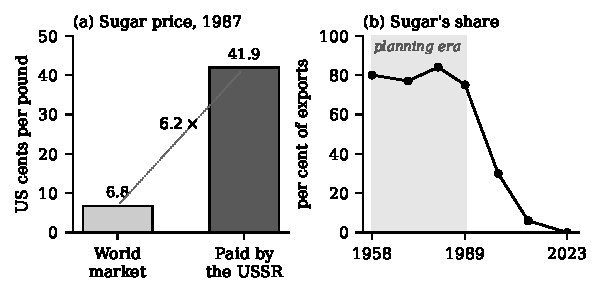
\includegraphics[width=\linewidth]{figs/comecon}
\caption{The subsidy, and what it bought. (a)~The mechanism: in 1987 the Soviet
Union paid more than six times the world price for Cuban sugar, and supplied oil
below it. (b)~The result: sugar's share of Cuban merchandise exports barely
moved across thirty years of planning, the highest investment rate in Latin
America and a Comecon membership organised around international specialisation
--- and then collapsed when the buyer went. A guaranteed price removes the only
signal that tells a producer to become good at something else. Panel~(a) is two
measured values rather than a series, because the year-by-year price data is not
reliably public and drawing a line through two points would invent the shape;
the post-1989 values in~(b) are estimates, flagged in \texttt{verify.md}. Generated by
\texttt{figs/comecon.py}.}
\label{fig:comecon}
\end{figure}

\section{The failure that mattered: no diversification}

Here is the fact that indicts the whole period, and Fig.~\ref{fig:comecon}(b) is its picture. In 1958, sugar was about four
fifths of Cuban exports. In 1989, after thirty years of planning, three decades
of the highest investment rates in Latin America, a Comecon membership
explicitly organised around international specialisation, and the best-educated
workforce in the region, sugar was still about three quarters of Cuban
exports \citep{onei,mesalago2000}.\unv{}

Everything else was small. Nickel, from the Moa and Nicaro deposits, was
second. Tobacco, citrus, fish and rum followed. The industrial base built in
the 1970s was assembly and import substitution for the domestic market, ran on
Soviet inputs, and could not export outside Comecon because its costs and
quality were set by a market that did not test either. A pharmaceutical and
biotechnology capability was started in the early 1980s --- of which much more
in Chapter~\ref{ch:life}, because it is the one exception and the one asset ---
but it was a decade from products in 1989.

The reason for the failure is not mysterious and it is not the embargo. A
protected market at guaranteed prices removes the only signal that tells a
producer to become better at something else. Cuba had, for eighteen years, the
sweetest terms of trade any small country has ever been offered, and it used
them to remain a sugar economy with a very good school system. That is the
central economic lesson of Part I, and Chapter~\ref{ch:premises} states it as a
constraint on the design: \emph{a guaranteed buyer at a political price is not
a market, and an economy built on one does not develop.} It applied to the
American sugar quota before 1959 and it applied to the Soviet protocols after,
and Chapter~\ref{ch:venezuela} will show it applying a third time to
Venezuelan oil.

\section{Rectification, 1986}

In 1980, under pressure from food shortages, Cuba opened free farmers' markets
where cooperatives and private farmers could sell surplus above their state
quota at whatever price the market bore. They worked: food appeared. They also
produced visible inequality --- intermediaries, some farmers doing very well,
prices the poorest could not pay --- and complaints about profiteering.

In 1986 Castro launched the Rectification of Errors and Negative Tendencies. It
closed the farmers' markets. It banned private house construction for sale and
much private artisanal work. It curtailed the enterprise bonus system of the
SDPE, denounced material incentives, revived voluntary labour and the
contingent brigades, and rehabilitated Guevara's economic thinking explicitly
by name.

The timing is the point. In 1986 the Soviet Union was beginning perestroika.
Cuba responded to its patron's turn toward markets by turning away from them,
and it did so eighteen months before the terms of trade that made the choice
affordable began to disappear. Rectification is the clearest single instance of
the pattern this book will name in Chapter~\ref{ch:ledgerch} and that recurs
through Part II: \emph{Cuba liberalises under duress and re-centralises as soon
as the pressure lifts, and the re-centralisation always arrives just before it
is least affordable.}

\begin{ledger}{the Soviet economy, 1963--1989}
\emph{Achieved.} Fourteen years of solid growth and the highest living
standards the revolution has produced. A universal social state financed to
completion. Mass housing through the microbrigades. Full employment, in the
sense that everyone had a job. Institutional forms --- a constitution, a party
congress, elected municipal assemblies, codified law --- where before there had
been improvisation by speech. An education system whose output was, and remains,
the country's best asset. The founding of a biotechnology capability that would
outlive everything else here.

\emph{Cost.} Thirty years of accumulation that left the export basket where it
was in 1958, three quarters sugar, because guaranteed prices removed the reason
to change it. An economy structurally dependent on transfers running between a
fifth and a third of national income, from a single patron, with no plan for
their ending. A hard-currency default in 1986 that has locked the country out
of credit markets ever since. An enterprise system that could not calculate,
and a workforce whose pay had been decoupled from what it did. And a decision
in 1986 to reverse the one reform that had visibly worked, taken at the last
moment when reversing it was still survivable.
\end{ledger}

\chapter{Abroad}
\label{ch:internationalism}

\section{Why a small poor island had a foreign policy}

For thirty years Cuba conducted a foreign policy several orders of magnitude
larger than its size, and any account of the period that treats this as
peripheral has missed how much of the country's resources, self-understanding
and reputation went into it. At its peak Cuba had tens of thousands of soldiers
in Africa, doctors and teachers in dozens of countries, and a claim on the
attention of the non-aligned world that no state of six million people has had
before or since.

Three motives ran together and it is not always possible to separate them.
There was conviction: the leadership genuinely believed in a global revolution
and acted on that belief at real cost. There was security: a country under
permanent threat from a superpower ninety miles away buys allies and buys
standing, and standing is a form of deterrence. And there was the patron: after
1972 Cuban military deployments in Africa were logistically impossible without
Soviet transport and finance, and they served Soviet purposes, which is not the
same as saying Moscow ordered them --- the Angolan intervention in particular
appears to have been decided in Havana and presented to Moscow afterwards.

\section{The guerrilla decade}

Through the 1960s Cuba supported armed insurgency across Latin America, in
Venezuela, Guatemala, Colombia, Peru, Bolivia and Nicaragua, and in Africa.
Almost all of it failed. The doctrine, elaborated by R\'egis Debray from
Guevara's writings, held that a small armed nucleus in the countryside could
create the conditions for revolution rather than waiting for them, which was a
misreading of Cuba's own case: the Sierra Maestra had succeeded alongside an
urban movement, a collapsing army and an isolated dictator, none of which the
doctrine required.

Guevara left Cuba in 1965 to apply it, first in the Congo, where the campaign
was a failure he documented himself with striking honesty, and then in Bolivia,
where he was captured and killed by the Bolivian army with CIA assistance in
October 1967. His death converted him into the most reproduced image of the
twentieth century and removed from Cuban politics the one figure whose prestige
was independent of Castro's.

The policy also cost Cuba with Moscow, which was pursuing peaceful coexistence
and had working relations with several of the governments Cuba was trying to
overthrow, and with the Latin American communist parties, which Havana was
denouncing as passive. The 1966 Tricontinental Conference in Havana was the
high point of Cuban third-worldism and close to the low point of Cuban--Soviet
relations.

The alignment was purchased back in 1968. In August, when Warsaw Pact tanks
entered Czechoslovakia, Castro went on television and endorsed the invasion. He
did so in a speech that conceded almost everything --- that the invasion
violated legality, that the socialist camp had no right to do it under the
rules it claimed --- and endorsed it anyway on the grounds that the alternative
was Czechoslovakia's drift to the West. The speech is the most revealing
document of Cuban foreign policy in the period, and the trade it embodied was
explicit within months: Soviet oil deliveries were increased, the economic
integration of the 1970s followed, and Cuban support for guerrilla movements in
Latin America was wound down.

\section{Africa}

Cuba's military engagement in Africa began in Algeria in 1963 and became large
in Angola in 1975.

When Portugal's empire collapsed, Angola's independence was contested by three
movements. The Soviet-aligned MPLA held Luanda; the FNLA advanced from Zaire;
and UNITA was backed from the south by South Africa, which invaded in October
1975 with an armoured column heading for the capital. Cuba's response,
Operation Carlota, began in November \citep{gleijeses2002}: troops flown in on Cuban and later Soviet
aircraft, stopping the South African advance short of Luanda. Within months
there were 36,000 Cuban soldiers in Angola. They stayed for sixteen years. Over
the whole period something like 300,000 Cuban military personnel and 50,000
civilians served there \citep{gleijeses2013}.\unv{}

The war's decisive phase came in 1987--88 around Cuito Cuanavale in the
south-east, where a Cuban and Angolan force stopped a South African offensive,
and then in a Cuban armoured push toward the Namibian border that changed the
military balance in the south-west. The battle's outcome is disputed in detail
--- both sides claim it --- but its consequence is not: the quadripartite
negotiations that followed produced South African withdrawal from Angola,
Namibian independence in 1990, and Cuban withdrawal, and they took place
because Pretoria concluded it could no longer hold the line militarily. Nelson
Mandela, released in 1990, went to Havana in 1991 and said so directly. Whatever
else is in the ledger, Cuba's contribution to ending South African control of
Namibia and to the pressure that ended apartheid is real, was paid for in Cuban
lives, and was not done for money.

Ethiopia is the other half of the record and it is much worse. In 1977--78
Cuba sent some 16,000 troops to defend Ethiopia against a Somali invasion of
the Ogaden --- defensible on its own terms, since Somalia was the aggressor and
Cuba refused to join the subsequent offensive into Somalia proper. But the
government being defended was the Derg of Mengistu Haile Mariam, which was in
the middle of the Red Terror, and Cuba's presence continued through it and
through the famine and the forced resettlements of the 1980s. Cuba had also
been the ally of Somalia and of the Eritrean independence movement before
switching sides, and the Eritreans, who had trained in Cuba, were now on the
other end of the guns. Whatever internationalism meant in Angola, in Ethiopia
it meant supporting a mass-murdering client of the same patron.

The official Cuban count of dead across all internationalist missions,
published in 1991, was 2,289.\unv{} The families were told what was necessary
and the coffins came home together, in a single ceremony, sixteen years of them
at once, in December 1989.

\subsection{The doctors}

Running in parallel, and outliving all of it, was medical internationalism.
The first Cuban medical brigade went to Algeria in 1963, fifty-six people, sent
by a country that had just lost half its own physicians \citep{kirk2015}. By the 1980s Cuban
doctors were working across Africa, Central America and the Caribbean, mostly
without charge, in places where no other country would send anyone. The Latin
American School of Medicine, founded later, trained foreign students free.

This is the origin of the reputation that Chapter~\ref{ch:life} will argue is
Cuba's most valuable intangible asset --- and, from the 2000s, of the country's
largest export earner, which is a different thing and carries its own problems
of pay, consent and conditions that Part II will take up honestly.

\section{Mariel}

In April 1980 a bus crashed through the fence of the Peruvian embassy in
Havana. The guards were withdrawn after a dispute over asylum, and within
seventy-two hours around 10,800 people were inside the embassy grounds. The
scale of it --- ten thousand people in a garden, in a country whose government
had said for twenty years that only a handful of \emph{gusanos} wanted to leave
--- was a shock from which the official narrative never quite recovered.

Castro's response was to open the port of Mariel and invite Cuban Americans to
come and collect their relatives by boat. Between April and October 1980 about
125,000 people crossed to Florida. The Cuban state used the opening to empty
some of its prisons and psychiatric hospitals into the boats --- the number is
disputed but the practice is not, and it was deliberate, both to rid itself of
a burden and to discredit the emigration as criminal. It also organised
\emph{actos de repudio}, mob demonstrations outside the homes of those leaving,
in which neighbours and co-workers were assembled to shout, throw eggs and
sometimes beat people who had announced their departure. Cubans were made to
brutalise their neighbours as a condition of their own standing.

The consequences ran both ways. In the United States, Mariel arrived in an
election year, overwhelmed Florida's capacity, was fixed in the public mind by
the criminal contingent, and did lasting damage to the standing of Cuban
immigrants generally. In Cuba, the memory of the repudiation mobs is one of the
sharpest wounds the revolution inflicted on its own society --- not because of
what the state did, but because of what it made ordinary people do to each
other, which is harder to forgive and harder to forget. Any reconciliation
process proposed in Part III has to have an answer for the \emph{acto de
repudio}, and the answer is not that it was long ago.

\section{The end of the decade}

Two events closed the period.

In June and July 1989 General Arnaldo Ochoa, a hero of the Angolan campaign and
one of the three or four most prominent officers in the country, was arrested,
tried and executed along with three others, and a group of senior Interior
Ministry officials including the de la Guardia brothers was convicted, on
charges of drug trafficking and corruption. The Interior Ministry was purged and
placed under military control. That the trafficking occurred is not seriously
disputed. Whether the trial was about trafficking is: Ochoa was popular, was
associated with the officers who had seen how the Soviet Union was changing, and
had reportedly been critical of the leadership. The proceedings were televised,
the confessions had the cadence of 1971, and no independent inquiry has ever
been possible. What is certain is that the affair removed the only figure in
Cuba with a military reputation comparable to the Castros', at the exact moment
the Soviet bloc was dissolving.

In April 1989 Mikhail Gorbachev came to Havana. The visit was correct and cold.
Cuba had already banned two Soviet magazines, \emph{Moscow News} and
\emph{Sputnik}, for spreading perestroika; Castro had already made the speech
that gave the period its slogan, \emph{socialismo o muerte}, socialism or
death. The Cuban position was that reform in the Soviet Union was a Soviet
matter and that Cuba would not follow. It did not follow. Nineteen months after
Gorbachev's visit the trade that had underwritten the country for eighteen
years began to stop arriving.

\begin{ledger}{abroad, 1963--1990}
\emph{Achieved.} A decisive military contribution to the defeat of South
African expansion in southern Africa, to Namibian independence, and to the
pressure that ended apartheid --- acknowledged by Mandela, paid for in Cuban
lives, and not paid for by anyone. Medical brigades in dozens of countries from
1963, the seed of Cuba's most durable asset and its eventual largest export.
A standing in the non-aligned world out of all proportion to the country's
size, which functioned as a real component of its security.

\emph{Cost.} A decade of exported insurgency that failed everywhere it was
tried and killed the people sent to try it. The endorsement of the invasion of
Czechoslovakia, made in full knowledge of what it was, as the price of oil. A
long deployment in support of the Derg through the Red Terror and the famine.
Sixteen years of war fought by conscripts whose families were told little and
whose dead came home in one ceremony. And at home, in 1980, the deliberate
mobilisation of ordinary Cubans to assault their departing neighbours ---
the one thing in this ledger for which no external necessity can be pleaded.
\end{ledger}


% ===========================================================================
\part{1990--2026}
% Thirty-six years of adjustment to the loss of a patron, in two cycles:
% liberalise under duress, recentralise when the pressure lifts, twice over.
% ===========================================================================

\chapter{The Special Period}
\label{ch:collapse}

\section{The stop}

What happened to Cuba between 1990 and 1993 has no close parallel among
countries not at war.

The Soviet bloc had taken roughly 85 per cent of Cuban trade. Comecon dissolved
in June 1991; the Soviet Union followed in December. The preferential sugar
protocols ended, the concessional oil ended, the spare parts ended, the credit
lines ended, and the machinery of an entire economy --- built over eighteen
years to Soviet standards, with Soviet inputs, for a Soviet market ---
discovered simultaneously that none of its three sides existed any more.

Cuban imports fell from about \$8.1 billion in 1989 to about \$2.2 billion in
1993, a fall of roughly three quarters in four years.\unv{} Oil imports fell
from around 13 million tonnes to around 6.\unv{} The official Cuban figure for the fall
in output is 34.8 per cent between 1989 and 1993, probably the largest
four-year decline in twentieth-century Cuba. It is also the \emph{lowest}
figure in circulation: Cuban media reported 48 per cent at the time, and
independent reconstructions have gone as high as 50 per cent
\citep{mesalago2005}. The spread turns
on the exchange-rate question of the note on sources rather than on any dispute
about what physically happened, and this book uses the official figure because
it is the most conservative one available and the argument does not need a
larger number. For comparison, the United States lost about 27 per cent of
output in the Great Depression, over four years, with its trading partners
still in place.

Fidel Castro named it in 1990: the Special Period in Time of Peace, a phrase
lifted from the civil-defence contingency plans drawn up in the 1980s for the
event of a war and a total blockade. The name was accurate. The plans had been
written for a siege, and a siege is what arrived, except that nobody was
besieging.

\section{What that was like}

The abstraction is useless without the texture, and the texture is what Cubans
who lived through it still measure everything against.

Electricity went first, because the thermal plants ran on imported fuel.
Blackouts of twelve to sixteen hours a day were normal by 1993, scheduled by
neighbourhood and then not scheduled at all. Without electricity there is no
water, because Cuban water is pumped; no refrigeration, in a climate where food
spoils in hours; no lifts in the apartment blocks the microbrigades had built;
and no light to read by in a country whose principal remaining asset was that
everyone could read.

Transport went next. Buses stopped for want of fuel and tyres. The state
imported over a million Chinese bicycles and built factories to assemble more,
and Havana --- a city with no bicycle tradition at all --- became a city of
bicycles, with the injuries and the exhaustion that implies in that heat. Later
came the \emph{camellos}, articulated trailers hauled by lorry tractors,
carrying several hundred standing passengers each. Oxen returned to fields that
had been mechanised for twenty years, and the state trained them and the men to
drive them, because there was no diesel.

Then food. The ration book had always been a floor and the state economy a
ceiling; now the ceiling collapsed onto the floor and the floor did not hold.
Average daily energy intake fell from roughly 2,900 kilocalories in 1989 to
somewhere around 1,860 in 1993, and protein intake fell by close to half.\unv{}
Cuban adults lost, on average, between five and ten kilograms. There was no
famine in the technical sense --- no mass starvation deaths, no localised
collapse --- but there was a country-wide, sustained, involuntary reduction in
food intake to below what an adult needs.

The clinical proof arrived in 1992. An epidemic of optic and peripheral
neuropathy spread across the island, blurring and in some cases destroying
vision. It ran from 1991 to 1994 and peaked over 1992--93, and the Cuban health
ministry's own count was 50,862 cases in a population of 10.8 million
\citep{mmwr1994}. The
cause was nutritional: B-vitamin deficiency, aggravated by tobacco and rough
alcohol, in a population that had been eating too little for two years. It was
halted by handing out vitamin tablets to the entire population, which is
simultaneously an indictment of the situation and a demonstration of what a
health system that reaches every block can do in a month. There were no deaths
from it, and fewer than one in a thousand of those affected were left with
lasting damage --- which is the same story as the infant mortality figures
below, and should be read the same way.

Everything else followed from those four. Soap and detergent disappeared, and
with them a measurable rise in diarrhoeal and skin disease. Tuberculosis
incidence roughly tripled from a very low base. Prostitution reappeared, aimed
at the tourists who were the only source of hard currency, and with it a word,
\emph{jineterismo}, that had not been needed for thirty years. The sugar
industry --- the thing the whole economy had been built around --- could not get
fertiliser, fuel or spares, and the harvest fell from 8.1 million tonnes in
1989--90 to 4.3 million by 1993 and 3.3 million by 1994--95. It never
recovered, in any year, ever again.

\section{What did not collapse}

Here the book has to be careful, because this is the single strongest piece of
evidence in favour of the Cuban model and it is routinely omitted by people who
find it inconvenient.

Infant mortality did not rise. It fell. In 1989 it was about 11.1 per thousand
live births; through the worst years of the Special Period it continued to
decline, and by 1994 it was under 10.\unv{} Life expectancy did not fall.
Immunisation coverage did not fall. No school closed. The universities stayed
open, on bicycles and candlelight. There was no epidemic of the classic
mortality signatures of economic collapse --- no surge in infant deaths, no
collapse of male life expectancy of the kind Russia recorded in exactly the
same years from exactly the same shock.

This is not a small thing and it should not be explained away. Russia in
1990--94 lost a comparable share of output and lost roughly six years of male
life expectancy with it. Cuba lost more output and lost none. The difference is
that Cuba's health and education systems were not financed out of the collapsing
sector; they were a prior claim on whatever remained, defended politically, and
staffed by people who kept coming to work in a country with no transport. When
this book argues in Chapter~\ref{ch:welfare} that the welfare state is the one
thing worth keeping, this is the evidence: a universal system with deep
territorial reach is a shock absorber of a kind that nothing else in a poor
country's toolkit can substitute for.

Two qualifications, both real. The systems degraded even where the outcome
indicators held --- hospitals without anaesthetics, without X-ray film, without
functioning sterilisers, and doctors who improvised or did without. And there
was one genuinely perverse benefit, documented afterwards and worth stating
because it shows how strange the episode was: the forced calorie restriction and
the forced physical activity produced a measurable fall in diabetes and
cardiovascular mortality across the 1990s, which reversed when weight was
regained after 1995 \citep{franco2013}.\unv{} A country lost weight because it was hungry and its
heart-disease deaths fell. That is not a policy recommendation. It is a reminder
that this period does not fit any simple story.

\section{Option Zero, and what came out of it}

The contingency planning went further than what was implemented. Option Zero was
the plan for the total loss of imported fuel: no electricity generation to
speak of, transport by animal, food produced and distributed at neighbourhood
level through communal kitchens, the country reorganised into self-supplying
cells. It was prepared and it was not needed, and that it was prepared says
something about how the leadership assessed 1992.

What was implemented, and what outlasted the crisis, was the agricultural
improvisation. Without fertiliser, pesticide or fuel, Cuban agriculture was
forced into low-input methods: biological pest control, composting, animal
traction, and above all the \emph{organop\'onicos}, raised-bed vegetable
gardens on vacant urban lots, which by the 2000s supplied a substantial share
of the fresh vegetables consumed in Havana. This became internationally famous
and is frequently over-claimed. What it demonstrably did was put vegetables into
cities. What it did not do was feed the country: Cuba's food import dependence
went up across the whole period, not down, and the case for low-input
agriculture has to be made on its merits in Chapter~\ref{ch:land} rather than
on a 1990s legend.

\section{August 1994}

By the summer of 1994 the currency had gone. The peso, official at one to the
dollar, traded on the street at 120 to 150. A state wage bought almost nothing.
People were leaving on anything that floated, and the state's practice of
intercepting boats had produced a series of violent incidents.

On 13 July 1994 a group of about seventy people hijacked an old tugboat, the
\emph{13 de Marzo}, and headed for Florida. It was pursued by state-operated
vessels which rammed it and directed high-pressure water hoses at the people on
deck, including at children being held up. The tug sank seven miles offshore.
Thirty-seven people died, ten of them children.\unv{} The government's account
was that the sinking was accidental and the fault of the hijackers. No
independent investigation was permitted. The Inter-American Commission on Human
Rights found the state responsible \citep{iachr1996}. Whatever one concludes about the Special
Period generally, this happened, and it happened to people trying to leave a
country that would not let them.

On 5 August 1994, after rumours that a boat would be allowed to depart,
thousands of people gathered on the Havana Malec\'on, threw stones, broke
windows, and shouted against the government. It was the first mass anti-
government demonstration in thirty-five years. It was put down within hours,
partly by police and partly by mobilised construction workers with sticks, and
Castro himself came to the seafront during it. The \emph{maleconazo} lasted an
afternoon and changed the government's calculation permanently.

Within days Castro announced that anyone who wanted to leave by sea could go
unhindered. Over the following five weeks something like 30,000 to 35,000 people
put to sea on rafts and inner tubes.\unv{} An unknown number drowned. The United
States, unable to absorb them, changed a thirty-year-old policy: rafters
intercepted at sea were taken to Guant\'anamo rather than to Florida, where
some 30,000 were held in camps for months. The negotiations that followed
produced the migration accords of September 1994 and May 1995, under which the
United States undertook to admit a minimum of 20,000 Cubans a year through
legal channels and to return those interdicted at sea, while those who reached
land could stay --- the policy that became known as wet-foot, dry-foot, and that
would shape Cuban emigration for the next twenty-two years.

The migration valve is the mechanism this book will keep returning to. Twice
before --- Camarioca in 1965, Mariel in 1980 --- and now a third time, internal
pressure was released by opening the door, and each time it worked. It is one of
the two instruments that have kept the Cuban political system stable through
crises that would otherwise have broken it, the other being the welfare floor.
Chapter~\ref{ch:crisis} will show the same valve opening a fourth time, on a
scale that finally threatened the thing it was protecting.

\begin{ledger}{the Special Period, 1990--1994}
\emph{Achieved.} A loss of over a third of national output absorbed without
famine, without epidemic mortality, without the collapse of the state, and
without the fall in life expectancy that the identical shock produced in
Russia. Infant mortality continued to \emph{fall} throughout. Every school
stayed open. The health system degraded severely and held its outcomes, which
is the strongest evidence in this book that a universal system with
territorial reach is worth the money it costs. Urban agriculture, born of
desperation, became a durable and genuinely useful institution.

\emph{Cost.} A country of readers reduced to roughly 1,860 kilocalories a day,
losing five to ten kilograms a head, with fifty thousand cases of nutritional
blindness as the clinical receipt. The sugar industry destroyed and never
recovered. A decade of consumption gone. Prostitution and a dollar economy
restored as facts of Cuban life. Thirty-seven people, ten of them children,
drowned off Havana in an incident the state has never independently
investigated. And the moment, on an August afternoon on the Malec\'on, when the
social contract of 1959 stopped being believed by the people it had been
written for.
\end{ledger}

\chapter{Reform, and its reversal}
\label{ch:dollarreform}

\section{Reform under duress}

Between July 1993 and the end of 1995 the Cuban government did more to
liberalise its economy than in the previous thirty-four years combined. It did
so reluctantly, described the measures throughout as temporary concessions
forced by circumstance, and withdrew as many of them as it could as soon as it
was able. That sequence is the subject of this chapter, and it is the clearest
single instance of the pattern this book has been assembling.

The measures, in order:

\emph{July 1993.} Possession of hard currency was decriminalised. Until that
month a Cuban caught with a dollar could be prosecuted; from that month Cubans
could hold, spend and receive dollars legally. This was the pivotal decision,
because it legalised remittances --- and remittances from the diaspora that
thirty years of policy had denounced as worms became, within a decade, one of
the largest sources of foreign exchange in the country.

\emph{September 1993.} Self-employment was re-legalised in 117 categories, later
extended to around 157. The list was a list: activity was permitted by
enumeration, not by right, and university-trained professions were excluded ---
a doctor could not practise privately, an engineer could not consult, but either
could rent a room or drive a taxi. This design decision, more than any other,
determined what the Cuban private sector became.

\emph{September 1993.} The state farms, which held most of the agricultural
land, were broken into Basic Units of Cooperative Production, the UBPCs, holding
land in usufruct with a nominal right to organise their own work. Roughly 40 per
cent of agricultural land changed hands on paper.\unv{} In practice the state
retained the procurement monopoly, the input supply and the price, so what was
devolved was the loss and not the decision. The UBPCs have underperformed the
private and older-cooperative sector continuously ever since.

\emph{October 1994.} Agricultural markets were reopened at free prices for
produce above the compulsory state quota --- the same measure that had been
introduced in 1980 and abolished in 1986. Food appeared in Havana within weeks,
at prices most people could not afford, which was also what had happened in
1980.

\emph{1994--95.} The fiscal and monetary stabilisation, which is the part of
this period that gets least attention and deserves the most. The budget deficit,
which had reached something like 30 per cent of output in 1993, was cut to
around 7 per cent in 1994 and to 2 per cent by 1996, through price rises,
subsidy cuts, new taxes under a 1994 tax law, and the removal of currency by
confiscatory means. Exchange houses were opened in 1995 at a market rate. The
informal exchange rate, which had reached 120 to 150 pesos to the dollar in mid-
1994, came back to around 20 to 25 by 1996 and stayed in that band for the next
twenty-five years \citep{mesalago2005}.\unv{} A currency that had been destroyed was
stabilised inside two years without external assistance. Chapter~\ref{ch:money} takes this
seriously as a precedent, because the same state did the opposite in 2021.

\emph{September 1995.} Law 77 opened foreign investment, permitting up to full
foreign ownership in principle, and creating the joint-venture form that most
foreign capital in Cuba has used since. It kept the feature that has done most
to deter investors: the foreign partner does not hire its own workers, but
contracts them from a state employment agency, pays the agency in hard currency,
and the agency pays the worker in pesos, keeping the difference. At an official
rate of one to one, this meant a worker whose employer paid the state several
hundred dollars a month received the peso equivalent of perhaps twenty.
Chapter~\ref{ch:capital} argues that this single arrangement has cost Cuba more
foreign investment than any American statute.

The measures worked. 1994 was the trough; growth resumed in 1995 and ran through
the second half of the decade. The economy that emerged, however, was not the
one that had gone in.

\section{The dual economy}

Cuba came out of the Special Period with two currencies, two price levels, two
labour markets and two populations.

The convertible peso, the CUC, was introduced in 1994 and pegged at one to the
dollar. Alongside it the ordinary peso continued, at twenty-four or twenty-five
to the CUC for households and --- this is the part that mattered --- at one to
one for state enterprise accounting. Cuba thus ran a twenty-five-fold
discrepancy between the rate its households faced and the rate its own firms
used to value imports, exports, costs and profits, for twenty-six years. Every
enterprise account in the country was fiction. No Cuban manager could tell
whether their operation created or destroyed value, and neither could the
ministry above them. This is not a technicality; it is the reason Cuban
industry could not be reformed even by people who wanted to reform it, because
nobody could identify which parts were worth keeping.

The social consequence was the inversion of the pyramid. A surgeon earned a
state salary in pesos. A bellhop earned tips in convertible currency. A
professor of literature drove a taxi in the afternoon; a research chemist rented
her spare room. The valuation the society had spent thirty years teaching ---
that education was the route to standing --- was contradicted daily and
publicly by the exchange rate. Cuba's Gini coefficient, which had been around
0.24 in the mid-1980s and was among the lowest measured anywhere, was around
0.40 by the end of the 1990s \citep{mesalago2005}.\unv{}

That inequality had a colour. The emigration of 1959--62 had been
overwhelmingly white; the remittances that flowed back thirty years later
therefore flowed overwhelmingly to white households, by margins that the
available surveys put at four fifths and above.\unv{} The tourist sector, the
other route to hard currency, hired front-of-house staff by \emph{buena
presencia} --- good appearance --- which in practice meant what it has always
meant. So the state that had abolished the colour bar in 1959 and then declared
the racial question closed in 1962, and had thereby made it unmeasurable for
thirty years, entered its market opening with foreign-currency access
distributed along the exact line it had stopped looking at.
Chapter~\ref{ch:premises} treats this as a hard constraint on any transition
design, and not as a historical note.

Tourism was the visible face of it. Arrivals went from about 340,000 in 1990 to
around 745,000 in 1995 and to about 1.8 million by 2000.\unv{} The plant was
built by joint ventures with Spanish, Canadian and Jamaican chains, mostly as
all-inclusive beach resorts at Varadero and the northern cays, physically
separated from the country around them --- and, until 2008, legally separated
too, since Cubans were not permitted in tourist hotels. A state that had made
its founding claim on the abolition of a foreigners' Cuba had rebuilt one, and
this time it was the government enforcing the door.

\section{The reversal}

By 1996 the emergency had passed, and the leadership's assessment of the
reforms changed with it.

The signal came in March 1996, when Ra\'ul Castro delivered a report to the
Central Committee attacking the Centre for the Study of the Americas, a party
research institute whose economists had been analysing the reforms and their
possible extension. The institute was dismantled and its researchers dispersed.
The message to Cuban social science was received and has never needed
repeating.

What followed was a decade of quiet reversal. Self-employment licences, which
had peaked at around 209,000 in early 1996, were squeezed by taxation, by
inspection, and by the withdrawal of categories, falling to roughly 150,000 by
2003 and lower after \citep{ritter2015}.\unv{} New licences in most categories were suspended
outright in 2003--04. In 2003 enterprises were required to hold and transact
their foreign currency through a single central account, ending the
decentralised access that had made the joint-venture sector function. In
November 2004 the United States dollar was withdrawn from circulation
altogether and a 10 per cent surcharge imposed on converting dollars into CUC,
which was presented as a response to American financial pressure and which also
happened to tax every remittance.

None of this was a return to 1968; the markets stayed open, the tourism sector
grew, the remittances kept coming. But the direction was unmistakable, and its
logic was consistent: the reforms of 1993--95 had been concessions extracted by
an emergency, and with the emergency over the concessions were withdrawn.

\section{Politics in the same years}

The reversal was not only economic, and the external environment did not help.

On 24 February 1996 Cuban air-force MiGs shot down two civilian aircraft flown
by Brothers to the Rescue, an exile organisation that had been searching for
rafters and dropping leaflets over Havana, killing four men. The location of the
shootdown --- inside or outside Cuban airspace --- was disputed; that the
aircraft were unarmed civilian light planes was not. The political consequence
in Washington was immediate: the Cuban Liberty and Democratic Solidarity Act,
Helms--Burton, which had been stalled, passed within weeks. It codified the
embargo into statute, so that it can now be lifted only by Congress and not by a
president; it extended sanctions to foreign companies trafficking in confiscated
American property; and its Title III created a right for American nationals to
sue such companies in American courts. Every president from Clinton onward
suspended Title III at six-month intervals until 2019.

Helms--Burton matters to Part III for a reason beyond its direct effect. It
converted American policy toward Cuba from an executive instrument, which can be
traded, into a legislative one, which must be repealed. Any Cuban reform design
that assumes the embargo will end when relations improve is assuming something
the American constitutional structure does not readily deliver, and
Chapter~\ref{ch:premises} therefore treats the embargo as a variable that may
not move.

Inside Cuba the same years produced Law 88 of 1999, which made collaboration
with United States policy punishable by up to twenty years and which is
sufficiently broadly drafted to cover most forms of independent journalism; and
then, in 2002, the Varela Project. Oswaldo Pay\'a and a network of Catholic lay
activists used Article 88 of the 1976 constitution, which permitted citizens to
propose legislation with 10,000 signatures, to submit 11,020 signatures asking
for a referendum on free expression, free association, an amnesty and free
elections. It was the most serious attempt to use the system's own rules against
it in forty years. The response was a counter-mobilisation that collected some
eight million signatures for a constitutional amendment declaring the socialist
character of the system irrevocable, which the National Assembly duly passed in
June 2002. The route Pay\'a had found was closed by constitutional amendment.

In March 2003, in the week the United States invaded Iraq, Cuban state security
arrested seventy-five independent journalists, librarians, trade unionists and
opposition organisers, tried them within weeks, and sentenced them to terms of
six to twenty-eight years. It is known as the Black Spring. In the same month
three young men hijacked a Havana Bay passenger ferry in an attempt to reach
Florida, took hostages, harmed nobody, surrendered when the boat ran out of
fuel, and were tried and executed by firing squad within nine days. Cuba's
standing with the European left, which had survived Padilla, largely did not
survive this. The wives and mothers of the seventy-five began walking to mass in
white every Sunday, and were still doing so, and being detained for it, twenty
years later.

\begin{ledger}{reform and reversal, 1993--2004}
\emph{Achieved.} An economy pulled out of free fall in eighteen months. A
destroyed currency stabilised without external assistance --- deficit from
about 30 per cent of output to 2 per cent, informal exchange rate from 150 to
25 --- which is a genuine technocratic accomplishment and the counter-example
to Chapter~\ref{ch:crisis}. Dollars, self-employment, farmers' markets and
foreign investment legalised. Tourism rebuilt from nothing to 1.8 million
visitors. A private sector of a few hundred thousand people re-created from
zero, and with it the first Cubans in a generation who did not depend on the
state for their income.

\emph{Cost.} A dual currency that made every enterprise account in the country
fictitious for twenty-six years, and thereby made the economy unreformable by
anyone, including those who wanted to reform it. Inequality up from among the
lowest measured anywhere to Latin American levels in a decade, distributed
along a racial line the state had spent thirty years declining to measure.
Tourist enclaves Cubans were legally barred from entering. A reform programme
withdrawn as soon as it was survivable to withdraw it, with the research
institute that had analysed it dismantled as a warning. Seventy-five people
imprisoned for terms up to twenty-eight years, and three shot, in a single
month.
\end{ledger}

\chapter{The Venezuelan decade}
\label{ch:venezuela}

\section{The third patron}

In October 2000 Fidel Castro and Hugo Ch\'avez signed an Integral Cooperation
Agreement in Caracas. Venezuela would supply Cuba with crude oil and refined
products on concessional terms --- initially some 53,000 barrels a day, rising
over the decade to around 90,000 or 100,000 --- and Cuba would pay, in
substantial part, not in money but in the services of its people: doctors,
nurses, dentists, teachers, sports trainers, agricultural technicians and
military and intelligence advisers.\unv{}

It is worth pausing on the structure of this deal, because it is the third time
the same structure appears in this book. In 1934 the United States guaranteed a
price for Cuban sugar above the world market and Cuba organised itself around
it. From 1972 the Soviet Union guaranteed a price for Cuban sugar and supplied
oil below the world market, and Cuba organised itself around that. From 2000
Venezuela supplied oil below the world market and bought Cuban services above
their market value, and Cuba organised itself around that. Each arrangement was
generous, each was political rather than commercial, each rescued the Cuban
economy at the moment it was struck, and each removed the pressure that would
otherwise have forced diversification. Chapter~\ref{ch:sovieteconomy} stated the
rule; this chapter is its third confirmation.

\section{Doctors as an export industry}

The exchange grew far beyond oil. From 2003, under the Barrio Adentro
programme, Cuba placed medical personnel in Venezuelan barrios and rural areas
where Venezuelan doctors had never practised --- at the peak something in the
range of twenty to thirty thousand health workers, with total Cuban civilian
personnel in Venezuela reaching perhaps forty thousand.\unv{} Similar
arrangements, smaller and mostly paid in cash, were signed with Brazil,
Angola, Algeria, South Africa, Qatar and dozens of other countries, and after
2013 the Mais M\'edicos programme placed some 11,000 Cuban doctors in
underserved regions of Brazil.

The economics of this transformed the country. By the early 2010s Cuba's
exports of professional services were worth on the order of eight to ten billion
dollars a year, of which health services were the large majority --- against
tourism at roughly two and a half billion and nickel at about one and a
half \citep{onei,mesalago2013}.\unv{} Cuba's largest export was no longer a commodity. It was its
doctors. That is a genuinely remarkable outcome for a country of eleven
million, it is the direct dividend of the investment described in
Chapter~\ref{ch:socialstate}, and it is the strongest existing evidence for the
proposition in Chapter~\ref{ch:talent} that Cuba's educated population is an
exportable asset.

The arrangement's other half has to be reported as plainly. The host government
paid Cuba; Cuba paid the doctor. The doctor's share was typically a small
fraction of the contract value --- in the Brazilian programme, the most
transparently documented, Cuba received roughly four times what it passed to the
physician \citep{kirk2015}.\unv{} Doctors on mission were subject to rules that would not be
accepted in most labour markets: in several destinations their passports were
held by the mission chief; movement, association and relationships with locals
were restricted; and a doctor who abandoned the mission was, until the
migration reform of 2013, barred from returning to Cuba for eight years, which
in practice meant separation from children. The United States operated a Cuban
Medical Professional Parole programme from 2006 to 2017 specifically to induce
defections, and several thousand took it.

Both descriptions are true at once, and the honest summary is that Cuba built a
real and valuable export industry and financed it partly by underpaying and
over-controlling the people who produced it. Chapter~\ref{ch:life} argues that
the programme should be kept and the labour arrangement changed, and that this
is not only the ethical answer but the revenue-maximising one, since the
industry's binding constraint is now the supply of willing doctors.

\section{What the money bought}

The Venezuelan relationship coincided with, and paid for, the most politically
confident period the Cuban government has had since the 1980s.

Abroad, it bought a bloc. ALBA was founded by Cuba and Venezuela in 2004 and
grew to include Bolivia, Nicaragua, Ecuador and several Caribbean states.
Petrocaribe, from 2005, extended Venezuelan concessional oil across the
Caribbean with Cuban medical missions attached. The regional isolation that had
been American policy since 1962 simply dissolved: the Organization of American
States revoked Cuba's 1962 suspension in 2009, the Community of Latin American
and Caribbean States was founded without the United States in 2011 and Cuba
chaired it in 2013, and the European Union's 1996 Common Position, which had
conditioned relations on democratisation, was steadily bypassed by member states
and formally replaced in 2016.

At home it bought the Battle of Ideas. This began in late 1999 with the case of
Eli\'an Gonz\'alez, a five-year-old boy who survived the sinking of his mother's
boat and was held in Miami by relatives against his father's wishes. Cuba
mobilised around his return for seven months, in daily marches and a permanent
tribune built opposite the American mission, and won: the boy went home in June
2000. It was the last unambiguous political victory the Cuban government won on
its own terms, and the mobilisation machinery it built was then turned to
domestic programmes --- an army of young social workers, university courses
delivered in every municipality, television as a teaching medium, and a great
deal of capital spending decided by mass campaign rather than by plan.

One of those campaigns deserves its own paragraph, because Part III depends on
it. By 2005 the Cuban grid was failing: the thermal plants were beyond their
design lives, unplanned outages were routine, and a hurricane season could take
the country dark. The Energy Revolution of 2006 attacked the problem from both
ends at once. On the demand side the state replaced essentially every
incandescent bulb in the country --- some nine million --- with compact
fluorescents, distributed millions of efficient rice cookers and pressure
cookers, and replaced the oldest refrigerators and air conditioners. On the
supply side it installed around four thousand small distributed generator sets,
roughly 1,300 megawatts in total, sited across the country rather than
concentrated in a few large plants.\unv{} Blackout hours fell sharply. The
programme was expensive, the generators burned expensive fuel, and the strategy
was later allowed to decay --- but the diagnosis was right, and it was right in
a way that matters now: Cuba's grid problem is best attacked by distributed
capacity and demand reduction, not by rebuilding large central plants.
Chapter~\ref{ch:energy} builds directly on this precedent, with the generators
replaced by photovoltaics and storage.

\section{Two shocks, and a credit history}

In August, September and November of 2008 three hurricanes --- Gustav, Ike and
Paloma --- crossed Cuba within ten weeks. Together they damaged or destroyed
something over half a million homes and caused losses conventionally estimated
at around ten billion dollars, on the order of a fifth of national
output.\unv{} It was the worst hurricane season in Cuban recorded history, and
it arrived in the same quarter as the global financial crisis.

Cuba's response to the resulting liquidity squeeze did lasting damage. Beginning
in late 2008 the state froze the bank accounts of foreign companies operating in
Cuba --- money those companies had earned and were entitled to repatriate,
amounting to something over a billion dollars --- and simply stopped paying
suppliers.\unv{} Some balances were released over the following years; some were
not. The measure solved a cash problem and created a reputation problem, and
the reputation problem has proved much more durable. Foreign companies now price
Cuban counterparty risk on the basis of what happened in 2009, and no statement
of intent from Havana has changed that. Chapter~\ref{ch:capital} argues that
this is a credit history, that credit histories are repaired by behaviour over
years rather than by legislation, and that any investment strategy which does
not begin by settling these arrears is proposing to build on a default.

\section{The end of it}

Hugo Ch\'avez was diagnosed with cancer in 2011 and was treated in Havana. He
died on 5 March 2013. Venezuela's own economy then entered the collapse that has
defined it since, and the terms Cuba had enjoyed began to erode --- shipments
falling year by year through the mid-2010s, and falling faster after 2016.

By then Cuba had had thirteen years of subsidised oil and a services export
boom, and had used them, as it had used the Soviet years, to postpone rather
than to restructure. The sugar industry was not rebuilt. Domestic food
production did not rise. The dual currency was not unified, although unification
was announced as policy in 2011 and prepared for a decade. The energy system was
not converted. What the country had instead was one more external rent, larger
than it looked, and a decade in which the pressure to change had been removed.

\begin{ledger}{the Venezuelan decade, 2000--2013}
\emph{Achieved.} An export industry built out of the education system that
displaced sugar, nickel and tourism combined, and that placed Cuban doctors in
places no other country would staff --- a real service really delivered, and
the best evidence available for the argument of Part~III. The end of Cuba's
regional isolation, with the OAS suspension revoked and CELAC founded and
chaired. The Energy Revolution of 2006, a correct diagnosis and a partially
correct cure, whose logic Chapter~\ref{ch:energy} adopts. Recovery from the
worst hurricane season on record without mass casualties, which is what a
civil-defence system with block-level reach is for.

\emph{Cost.} The third guaranteed buyer at a political price in seventy years,
taken for the third time, with the third identical result: no diversification,
no restructuring, and a cliff at the end of it. An export industry financed by
paying its workers a fraction of their contract value and, in several
destinations, holding their passports. The freezing of foreign companies'
accounts in 2009, which bought a year of liquidity at the price of a credit
history that is still being paid for. And thirteen years in which every
structural problem this book has named was identified, announced as policy, and
not fixed.
\end{ledger}

\chapter{Ra\'ul's decade}
\label{ch:raul}

\section{A different kind of governing}

Fidel Castro fell ill on 31 July 2006 and never resumed office; Ra\'ul Castro
took over provisionally that day and formally in February 2008. The change in
style was immediate and larger than the change in policy.

Fidel governed by speech: problems were named in public, solutions were
announced as campaigns, and the campaign was the instrument. Ra\'ul governed by
meeting. He delegated, set deadlines, demanded that ministries answer for
targets, and --- most unusually --- said in public that the system did not work.
The Camag\"uey speech of 26 July 2007 is the text: he told an audience that
Cuban wages were insufficient to live on, that structural and conceptual changes
were needed, and, in the example everyone remembers, that a country that could
not put a glass of milk on a child's table every day had a problem it should
stop explaining and start solving. Coming from the second man of the revolution,
in the anniversary speech, this was licence to discuss things that had not been
discussable.

He also opened a consultation. In late 2010 the draft economic guidelines were
circulated for discussion in workplaces and neighbourhoods; the government
reported some 160,000 meetings and millions of comments, and around two thirds
of the draft's paragraphs were modified \citep{mesalago2013}.\unv{} Whatever one makes of the
mechanism, this was the widest formal consultation the Cuban state had ever run,
and Cubans engaged with it seriously because they believed something would come
of it.

\section{The removal of humiliations}

The first measures were not economic reforms at all. They were the repeal of
prohibitions whose only function had been to remind Cubans of their position.

In 2008 Cubans were permitted to buy mobile telephones, computers, DVD players
and microwave ovens, and to stay in tourist hotels --- ending, twelve years
late, the situation in which a Cuban could not enter a building on Cuban soil
that a foreigner could. In 2011 they were permitted to buy and sell their own
houses and cars, which had been prohibited since 1960 and had produced an
elaborate grey market of swaps, fictional marriages and bribes.

And in October 2012, effective January 2013, the exit permit was abolished. The
\emph{tarjeta blanca} --- the white card, the permission-to-leave that had cost
money, taken months, required a letter of invitation, and been refused at
discretion --- was gone, and a Cuban could travel on a passport like anyone
else. Doctors and some other categories remained restricted in practice, and the
eight-year bar on returning was reduced to two. But the principle changed: after
fifty-four years, leaving Cuba temporarily stopped being a political act.

None of this cost the state anything. That is precisely the point, and
Chapter~\ref{ch:sequence} makes it an operating principle: the first phase of
any reform programme should begin with the prohibitions that cost nothing to
remove, because they are free, they are immediate, and they buy the credibility
that the expensive measures require. Ra\'ul Castro's most popular acts were all
of this kind.

\section{The guidelines, and why they stopped}

The Sixth Party Congress of April 2011 --- the first in fourteen years ---
adopted 313 Guidelines for Economic and Social Policy. The programme they
described was coherent: shrink the state payroll, expand non-state employment,
decentralise enterprise decisions, separate state administration from enterprise
management, unify the currency, and move from universal subsidy toward targeted
assistance. The announced first step was the transfer of half a million workers
off the state payroll within six months, and eventually more than a million.

The instruments were real. Self-employment was expanded to 178 and then 201
categories and the number of licence-holders rose from about 157,000 in 2010 to
over half a million by 2015 --- roughly a fifth of the employed
workforce \citep{ritter2015}.\unv{} Land was granted in usufruct under Decree-Law 259 of 2008,
initially 13 hectares, and under Decree-Law 300 of 2012 up to 67, to anyone
willing to farm it; something over 1.7 million hectares of idle land were handed
out.\unv{} Non-agricultural cooperatives were authorised on a pilot basis in
2013. The payroll reduction was never executed at anything like the announced
speed, because there was nowhere for the workers to go.

The reforms stalled, and the reason they stalled is the most useful thing in
this chapter for Part III, so it is worth stating precisely rather than
attributing to a general reluctance.

A Cuban private business between 2011 and 2021 had no legal personality. It was
a licensed individual, not a firm. It therefore could not sign a contract as an
entity, could not be sued or sue, could not own assets separately from its
owner, and could not, in most cases, be sold or inherited as a going concern.

It had no wholesale market. A restaurant bought its ingredients in the same
retail shops as households, at retail prices, competing with households for the
same scarce goods --- which is both economically absurd and the source of the
enduring popular complaint that the private sector caused the shortages.

It had no import rights. Everything had to be bought domestically or carried in
personal luggage by \emph{mulas}, travellers making repeated trips with
suitcases, which is how a substantial share of Cuban private-sector inputs
actually arrived for a decade.

It had no credit. Bank lending to the private sector was announced, hedged with
conditions, and never materialised at scale.

It had no access to foreign exchange at any usable rate.

And it operated by enumeration, not by right: an activity was legal if it
appeared on a list the state could shorten at any time, and the list was written
in the vocabulary of trades --- \emph{barber}, \emph{button-coverer},
\emph{party clown} --- with the professions excluded. A software developer had
no category. A design studio had no category.

The result is that Cuba got the private sector its rules were designed to
produce: several hundred thousand micro-operators in food, transport, lodging
and personal services, and essentially nothing in manufacturing, technology or
anything requiring an entity, a contract and a supply chain.
Chapter~\ref{ch:capital} treats this diagnosis as its starting point, because
almost every constraint in the list above is legal and internal, could be
removed without a dollar of foreign investment, and was not removed for a
decade.

\section{The opening}

On 17 December 2014 Ra\'ul Castro and Barack Obama announced simultaneously,
from Havana and Washington, that their countries would restore diplomatic
relations. The immediate exchange was the release of the American contractor
Alan Gross and of a Cuban-held intelligence asset, for the three remaining
members of the Cuban Five; behind it lay eighteen months of secret talks brokered
in Canada and by the Vatican \citep{leogrande2014}.

Embassies reopened in July 2015. Obama visited Havana in March 2016 --- the
first sitting American president since Coolidge in 1928 --- and gave a speech,
broadcast live on Cuban television, in which he said the embargo would end and
addressed Cubans directly about their own future. Regular flights resumed;
cruise ships docked; Airbnb entered the market in 2015 and had tens of thousands
of Cuban listings within two years; American visitors rose from around 91,000 in
2014 to over 600,000 in 2017, on top of a much larger flow of Cuban
Americans.\unv{}

For the Cuban private sector this was the best eighteen months it has ever had.
The demand went overwhelmingly to the non-state economy, because that is where
Americans on people-to-people licences were required to spend: private
restaurants, private rooms, private taxis, private guides. Money entered
households rather than the state, capital equipment came in with the visiting
relatives, and for the first time since 1959 there was a visible, growing,
domestically-owned Cuban middle class making its living from foreigners without
the state as intermediary.

That is also, precisely, why it was stopped.

\section{The brake}

The Seventh Party Congress of April 2016 was where the guidelines slowed. The
tone of the documents shifted from expansion of the non-state sector to its
regulation, and the phrase that circulated was the warning against the
concentration of wealth and property. In August 2017 the state suspended the
issue of new licences in a set of the most successful categories --- private
restaurants, room rentals, and others --- pending a review that lasted more than
a year and ended in a tighter regime: one licence per person, caps on the size
of restaurants, and stricter inspection.

Two further things happened in the same short period. Fidel Castro died on 25
November 2016. And on 8 November 2016 Donald Trump was elected, and in June 2017
issued a policy memorandum that reversed a substantial part of the opening ---
restricting individual people-to-people travel, prohibiting transactions with a
list of military-linked entities, and beginning the sequence of measures that
Chapter~\ref{ch:crisis} takes up.

It is tempting, and common, to attribute the closing entirely to Washington. The
sequence does not support it. The licence freeze of August 2017 was a Cuban
decision, taken about Cuban businesses, before the American measures had bitten.
Havana and Washington arrived at the same conclusion for opposite reasons:
that the growth of an independent Cuban private sector was politically
consequential. One of them wanted it and stopped subsidising it; the other did
not want it and stopped permitting it.

Ra\'ul Castro handed the presidency to Miguel D\'iaz-Canel in April 2018,
remaining First Secretary of the party until 2021. He left a country with a
larger private sector, a freer citizenry and a functioning relationship with the
United States, and with every structural problem identified in 2011 --- the dual
currency, the state payroll, enterprise autonomy, food production ---
diagnosed, announced, and unresolved.

\begin{ledger}{Ra\'ul's decade, 2006--2018}
\emph{Achieved.} The repeal of prohibitions that had no purpose but humiliation:
hotels, phones, computers, the sale of houses and cars, and above all the exit
permit, which after fifty-four years made leaving Cuba temporarily an ordinary
act. A private sector taken from 150,000 to over half a million people, about a
fifth of the workforce. Idle land distributed in usufruct on a large scale. A
national consultation the population took seriously. Diplomatic relations with
the United States restored, embassies reopened, and eighteen months in which
American demand flowed directly into Cuban households.

\emph{Cost.} A reform programme whose own instruments were designed so that it
could not succeed: no legal personality, no wholesale market, no import rights,
no credit, no foreign exchange, and legality by enumerated list. The result was
several hundred thousand micro-operators and nothing above them, which is
exactly what those rules produce. The one measure that would have made the
economy legible --- currency unification --- was announced in 2011 and deferred
for a decade, and would eventually be attempted at the worst possible moment.
And the opening that worked best was braked from the inside, in August 2017,
before Washington closed it from the outside.
\end{ledger}

\chapter{The crisis}
\label{ch:crisis}

\section{A note on writing about the present}

This chapter comes closest to the day it was written, and the closer it comes
the less certain it gets. Cuban statistical publication thinned after 2020;
several series in the \emph{Anuario} stopped appearing or appeared very late;
and the figures for 2025 and 2026 that circulate are in most cases estimates by
independent economists and demographers rather than published data. Where this
chapter gives a recent number it says whose number it is, and the figures for
the last two years should be read as provisional and checked against whatever
has been published since. The direction of every one of them is not in doubt.

\section{A new president, and a new constitution}

Miguel D\'iaz-Canel became president in April 2018 and First Secretary of the
party in April 2021, when Ra\'ul Castro retired. He is the first Cuban leader
since 1959 not named Castro and the first who did not fight in the
insurrection, and neither fact has translated into much independent authority.

His first substantial act was a constitution. The 2019 text, approved in a
February referendum, is a more liberal document than the 1976 one it replaced
and this should be said before the qualification. It recognises private
property and foreign investment as components of the economy rather than as
tolerated exceptions; it restores the presumption of innocence and habeas
corpus; it limits the president to two five-year terms and imposes an age limit
on first election; it re-creates the office of prime minister; it strengthens
the language on non-discrimination. Against that, it retains the Communist
Party as the superior leading force of society and the state, and it retains
the irrevocability of socialism that had been inserted in 2002 to bury the
Varela Project. It is a reform of the state's administration and not of its
politics.

The draft had contained a definition of marriage that would have permitted
same-sex marriage; it was withdrawn after organised opposition from evangelical
churches and referred to a future family code. That code was put to a separate
referendum in September 2022 and passed with about two thirds of the vote,
making Cuba one of the few countries in the world to legalise same-sex marriage
by popular vote. It is a genuine liberal advance and it was delivered by
referendum, which is worth noting in a chapter that is otherwise unrelieved.

\section{The re-tightening}

Between 2017 and 2020 the United States imposed a long series of measures ---
the figure usually cited is 243 --- that reversed the opening and went beyond
it.\unv{} Cruise ship calls were prohibited in June 2019. Individual
people-to-people travel was ended. Remittances were capped and then, in late
2020, effectively cut off when Western Union closed its more than four hundred
Cuban offices after the US Treasury designated the military-linked processor
through which they ran. Title III of Helms--Burton was allowed to come into
force in May 2019 for the first time since 1996, exposing any company using
confiscated property to suit in American courts. And in January 2021, in the
last week of the Trump administration, Cuba was returned to the list of state
sponsors of terrorism, a designation whose practical effect is less in its own
prohibitions than in the behaviour it induces in banks, which de-risk by
refusing Cuban business entirely.

The Biden administration eased parts of this from 2022 --- remittance caps
lifted, group travel restored, consular processing resumed in Havana --- and in
January 2025 removed the terrorism designation, which was reinstated within days
of the change of administration. The net effect over the decade is that the
external environment tightened, that the tightening was concentrated on exactly
the flows that reached Cuban households rather than the Cuban state ---
remittances, independent travel, private accommodation --- and that Cuban
policy toward its own private sector, described in the previous chapter, had
begun tightening first.

Meanwhile the Venezuelan subsidy shrank with Venezuela. Oil deliveries that had
been near 100,000 barrels a day fell to a fraction of that, with the shortfall
covered irregularly by Russia, Mexico and spot purchases the country could not
reliably pay for.

\section{Two years with the borders shut}

Tourism had reached about 4.7 million visitors in 2018. It fell to roughly 1.1
million in 2020 and to something under 400,000 in 2021.\unv{} For an economy in
which tourism was the second or third source of foreign exchange and the first
source of demand for the private sector, closing the borders for two years was
equivalent to closing the private economy. Arrivals recovered to around 2.4
million by 2023 and then stalled below that, at roughly half the pre-pandemic
level, while the Caribbean as a whole recovered fully --- a divergence that has
more to do with blackouts, hotels without water and empty shops than with
American policy.\unv{}

Against this, the pandemic produced the one unambiguous Cuban success of the
period. Cuba's biotechnology sector developed its own COVID-19 vaccines ---
Abdala at the Centre for Genetic Engineering and Biotechnology, Soberana~02 and
Soberana Plus at the Finlay Institute --- ran its own trials, reported
efficacies above 90 per cent, manufactured at national scale, and vaccinated
over 90 per cent of the population with domestically produced product,
including children from the age of two earlier than most of the
world.\unv{} No other country in Latin America did this. Cuba
did it while unable to import syringes reliably.

The qualification belongs with it: the vaccines were not submitted through, or
did not complete, the international prequalification and regulatory pathways
that would have allowed them to be sold at scale abroad, which is the same
failure Chapter~\ref{ch:life} identifies across the whole sector --- excellent
science, no regulatory conversion, and therefore very little money. Cuba
vaccinated itself and could not sell the result.

\section{Tarea Ordenamiento}

On 1 January 2021 --- in the middle of a pandemic, with the borders closed,
tourism at zero and the economy having contracted by about 11 per cent the
previous year --- the government executed the currency unification it had been
preparing since 2011.

The convertible peso was abolished with a six-month conversion window. The
official exchange rate for enterprises went from one peso to the dollar to
twenty-four, a devaluation of 2,300 per cent applied at a stroke to every
balance sheet in the country. Wages and pensions were raised several-fold to
compensate, the minimum wage going to 2,100 pesos. Subsidies were cut and many
regulated prices raised.

The direction was right and had been right for twenty years. Chapter~\ref{ch:dollarreform}
explained why: with two rates twenty-five-fold apart, no Cuban enterprise
account meant anything, and nothing could be reformed because nothing could be
measured. The execution was catastrophic, and the reasons are specific enough to
be instructive.

It was done with no reserves. A fixed rate is a promise to sell dollars at that
rate, and Cuba had no dollars, so the promise was not kept and a parallel rate
appeared immediately.

It was done with no supply response. Wages were multiplied in an economy where
the quantity of goods was falling, which is the definition of an inflation.

It was done with the private sector still repressed --- the licence freeze of
2017 was still in effect, and the small and medium enterprise law was eight
months away --- so the one part of the economy that could have responded to
higher prices with more output was not permitted to.

And it was done at the bottom of the worst external shock since 1993, when the
correct sequence is to stabilise first and unify afterwards.

The results followed. Official consumer price inflation was around 77 per cent
in 2021 and remained in the high double digits for the following two years,
with independent estimates considerably higher for the goods people actually
buy.\unv{} The informal exchange rate, which the reform was meant to eliminate,
detached from the official one and kept going: past 100 pesos to the dollar in
2022, past 200 in 2023, past 300 in 2024, and beyond that since.\unv{} Real
wages and pensions ended lower than before the reform that had multiplied them.
Cuban savings were destroyed for the second time in thirty years.

Chapter~\ref{ch:money} is written against this chapter. The lesson is not that
unification was wrong. It is that a monetary reform without reserves, without a
supply response and without a stabilisation programme in front of it is not a
reform but a devaluation of the population's savings, and that the same state
had demonstrated in 1994--96, with fewer resources and greater competence, how
to do it in the right order.

\section{11 July 2021}

On the morning of Sunday 11 July 2021 people came into the street in San
Antonio de los Ba\~nos, a town of forty thousand south-west of Havana. It was
filmed and put on Facebook. Within hours there were demonstrations in dozens of
towns and cities across the island --- the counts run from about forty to over
sixty locations --- including Havana, Santiago, Camag\"uey, Holgu\'in,
Cienfuegos, Matanzas and Palma Soriano.\unv{}

Nothing like it had happened since 1959. The \emph{maleconazo} of 1994 was one
city on one afternoon. This was national, simultaneous, and organised by nobody
--- which is exactly what made it uncontainable and, for the government,
incomprehensible. The immediate causes were blackouts in a July heatwave, empty
pharmacies during the worst COVID wave Cuba had, food queues, and the price
shock of the ordenamiento. The demonstrators were overwhelmingly young, poor,
and disproportionately from the Black and mixed-race neighbourhoods that
Chapter~\ref{ch:dollarreform} identified as the households without remittances
--- which is to say, from the constituency the revolution has always counted as
its own.

The response was mobile internet shut off nationally within hours; the
president's televised instruction, the \emph{orden de combate}, calling
revolutionaries into the street; deployment of special forces and of civilian
brigades; and mass arrests. One protester, Diubis Laurencio Tejeda, was shot
dead in La G\"uinera in Havana. Cubalex and Justicia~11J, the two monitoring
groups that did the counting because nobody official would \citep{justicia11j}, documented 1,481
people deprived of liberty in connection with the protests, of whom 57 were
under eighteen. Around 600 were prosecuted; at least 141 were charged with
sedition; and sentences ran from four years to thirty. Three years on, several
hundred were still in prison. The prosecutions were not of an organisation,
because there was no organisation; they were of individuals who had walked in
the street.

This is the central political fact of the period and Part III has to be answerable
to it. A government whose claim to legitimacy rests on having lifted the poor
and the Black out of the republic's neglect responded to a demonstration by the
poor and the Black with twenty-year sentences. Whatever the design in Part III
proposes about reconciliation, amnesty and the sequencing of political opening,
11 July 2021 and its prisoners are the case it has to be able to handle.

\section{The state's own retreat}

In August 2021, six weeks after the protests, the government did the thing it
had refused to do for a decade: Decree-Laws 46 to 49 created small and medium
enterprises with legal personality. A Cuban private business could at last be a
firm --- own assets, sign contracts, hire, and import and export through a state
intermediary. Some eleven or twelve thousand were approved over the following
three years, the large majority private, and they rapidly became a significant
share of the country's imports of food and consumer goods.\unv{}

The reform was real and it was also, transparently, a surrender: the state
legalised private importers because it could no longer stock its own shops.
The same logic produced the partial re-dollarisation of retail from 2024 ---
new state shops selling in dollars only, to capture remittances --- which
reintroduced, three years after abolishing it, a two-currency retail economy
with the currency of the poor on the wrong side of it.

And the enterprises arrived into a policy environment that turned on them
almost at once. From 2024 came price caps on private traders, restrictions on
what could be imported, higher taxes, and a public argument from the leadership
that the new firms were the cause of inflation rather than a response to it. The
pattern of 1996 and of 2017 repeated on a two-year cycle.

\section{The lights}

Cuba's electricity system reached the end of its life in 2024.

The generating fleet is a small number of large oil-fired thermal units, most
built between the 1960s and the 1980s, running past their design lives on heavy
domestic crude they were not built for, without maintenance, without spares, and
frequently without fuel. Through 2023 and 2024 daily deficits of a third or more
of demand were routine, and blackouts of twelve to twenty hours were normal
outside Havana and increasingly normal inside it.

The scale of the retreat is visible in the output. Cuba generated on the order
of 20 terawatt-hours in 2018; in 2023 it generated 15.3, of which 3.7 --- close
to a quarter --- was lost in transmission and distribution before reaching
anybody.\unv{} Consumption per head fell from about 1,856 kilowatt-hours in
2018 to 1,387 in 2023.

On 18 October 2024 the Antonio Guiteras plant, the largest single unit in the
country, tripped, and the entire national grid collapsed. Cuba went dark ---
eleven million people, every province, no exceptions. Restoration took several
days and failed twice during the attempt. It happened again in November after
Hurricane Rafael, and again in December, and again in 2025.\unv{} A national
blackout is not a shortage; it is the failure of the system as a system, and
once a grid has collapsed it collapses more easily.

The government's answer is solar, financed and built by China: a programme
announced around 2024 of dozens of photovoltaic parks with a first target near a
thousand megawatts, of which several hundred megawatts were reported energised
during 2025.\unv{} The direction is right --- Chapter~\ref{ch:energy} argues it
is the only direction available --- but photovoltaic capacity without storage
does not address a demand peak that occurs after sunset, and it does not by
itself restart a thermal fleet that must still cover the night.

Everything else in this chapter is downstream of the lights. Without stable
power there is no water pumping, no refrigeration, no food processing, no
tourism worth the name, no hospital that can plan a list, no remote work, and no
industry. Chapter~\ref{ch:premises} therefore treats electricity as the binding
constraint on the whole design and puts it before every other sector.

\section{The exodus}

The largest emigration in Cuban history took place between 2021 and 2025, and it
dwarfs the ones this book has already described.

The route ran through Nicaragua, which removed visa requirements for Cubans in
November 2021, and then overland to the United States border. In the American
fiscal year 2022 US authorities recorded something over 220,000 encounters with
Cuban nationals, and about 200,000 the following year; a humanitarian parole
programme opened in January 2023 admitted tens of thousands more by air; and
substantial numbers went to Spain under a 2022 descent-based nationality law, to
Mexico, Uruguay, Serbia and elsewhere.\unv{} Reasonable estimates of total
departures over 2021--2025 run from about one million to something approaching
two, against a population that had been about 11.2 million.

The official statistics office put the resident population at 9.7 million in
2024 --- a fall of 1.4 million in four years, and the first time it has been
below ten million since the 1980s --- with the 2024 census postponed.
Independent Cuban demographers, working from birth, death and border data, put
the true resident figure lower still, one study at around eight million, and
Albizu-Campos estimates roughly 1.79 million departures over 2021--24
alone \citep{onei}.\unv{} The uncertainty is large and the fact is not: Cuba has lost
something like a tenth to a fifth of its people in five years, and they were
disproportionately of working and child-bearing age.

This lands on a demography that was already among the oldest in the hemisphere.
Fertility has been below replacement since 1978 --- there is no cohort in the
pipeline --- and by the mid-2020s the total fertility rate was around 1.2 to
1.4, among the lowest in the world, with more than a quarter of the population
over sixty.\unv{} A pension system, a health system and a tax base all depend on
a ratio of workers to dependants, and that ratio has now moved further and
faster in Cuba than in any country not at war.

Chapter~\ref{ch:welfare} treats this as the hardest number in the book, and
Chapter~\ref{ch:talent} draws the conclusion that follows from it: a country
that has lost this many working-age people cannot be designed as though labour
were abundant. Every proposal in Part III is labour-constrained.

\section{Where the country stands}

In 2026 Cuba is poorer, older, smaller, darker and hungrier than at any point
since 1994, and by several measures than at any point since 1959.

Output has contracted in most years since 2019 and the cumulative fall is
large.\unv{} Sugar, which was 8.5 million tonnes in 1970 and 4 million as
recently as the 2000s, produced a harvest measured in the low hundreds of
thousands of tonnes in the mid-2020s --- less than in the nineteenth century ---
and Cuba now imports sugar.\unv{} The rationed basket is delivered late and
incomplete, and in 2023 the government asked the World Food Programme for
assistance with powdered milk for children, which it had never previously
done.\unv{} Medicines are absent from pharmacies at rates the health ministry
itself has acknowledged. Doctors and nurses are emigrating, and so are teachers.
The blackouts continue.

Against that: the schools are open, the clinics are staffed however thinly, the
vaccination programme still runs, violent crime remains low by regional
standards, and the state has not lost control of the territory. The floor that
held in 1993 is thinner and it is still there. It is the thing Part III is
written to save.

\begin{ledger}{the crisis, 2018--2026}
\emph{Achieved.} A constitution that recognises private property and restores
habeas corpus, and a family code legalising same-sex marriage passed by
referendum. Three domestically developed COVID-19 vaccines and a population
vaccinated with them, alone in Latin America. Private firms with legal
personality at last, after a decade of refusal. A currency unification that,
whatever its execution, ended a twenty-six-year accounting fiction. Solar
capacity begun. And a state that has kept schools open and clinics staffed
through a contraction it has not been able to stop.

\emph{Cost.} A monetary reform executed with no reserves, no supply response and
the private sector still shut, which destroyed the population's savings for the
second time in thirty years. Twelve-to-twenty-hour blackouts and four national
grid collapses. Sugar production below nineteenth-century levels and an appeal
to the World Food Programme for children's milk. The largest emigration in
Cuban history --- between one and two million people in five years, from a
population of eleven --- onto the oldest demography in the hemisphere. And, on
11 July 2021, sentences of up to thirty years, including of minors,
handed to poor and mostly Black Cubans for walking in the street to say there
was no food and no electricity.
\end{ledger}

\chapter{The balance sheet}
\label{ch:ledgerch}

This chapter does not narrate. The previous ten have done that. This one audits:
for each domain, what sixty-seven years produced, stated once, with both sides,
and the causal question asked rather than assumed. It is the hinge of the book,
because it is where the record turns into the constraint set that Part III has
to design within.

\section{Health}

\emph{What the record shows.} Cuba took a country with the best health
indicators in Latin America and a rural half with none of them, closed the
rural--urban gap, and held the national outcomes for sixty years through two
economic collapses. Life expectancy went from around 62 in 1958 to the high
seventies, converging with the United States on a fraction of the spending.
Infant mortality went from around 37 per thousand to single digits and stayed
there --- including through 1990--94, when it continued falling while national
output fell by a third. Polio, measles, diphtheria, rubella and neonatal tetanus
were eliminated. The delivery model, a polyclinic and then a family doctor
responsible for a defined population, is the mechanism, and it has been copied
deliberately by other countries because it works.

\emph{What has happened since 2019.} The system is being hollowed out from three
directions at once. Pharmaceutical supply has collapsed: the domestic industry
cannot obtain inputs and the state cannot pay for imports, and pharmacies are
empty at rates the health ministry itself acknowledges. Physical plant has
degraded past the point where outcome indicators can be maintained by staff
effort --- hospitals without reliable water, power or sterilisation. And the
staff are leaving, in the general emigration and through the medical missions.
Cuba's physician numbers remain high on paper because the paper counts doctors
on mission abroad.

\emph{The honest reading.} The achievement is real, was not bought by
measurement games, and is the single most valuable thing in this ledger. It is
also, in 2026, being lost in real time, and it will not survive another five
years of the present trajectory. That is the argument for
Chapter~\ref{ch:welfare} and the reason it is placed early: the asset is
depreciating faster than the plan can be written.

\section{Education}

\emph{What the record shows.} Illiteracy eliminated in a year and kept
eliminated. Universal primary and secondary schooling. Attainment measured by
an outside body two standard deviations above the Latin American mean, with the
poorest Cuban quartile outperforming the regional average --- which is the
number that matters, because it says the system compresses rather than
reproduces advantage. Higher education free and expanded by an order of
magnitude. Women's attainment ahead of men's since the 1980s.

\emph{The cost side, and the erosion.} The curriculum was a political
formation system, entire disciplines were closed or reduced to catechism, and
Cuba consequently has excellent engineers and physicians and very few people
trained to think about how a market, a court or a company works --- which is a
direct constraint on Part III's implementability, not a matter of taste. And the
system is eroding now: teachers are leaving for the private sector and for
abroad, enrolment in teacher training has fallen, and an informal private
tutoring economy has appeared to fill the gap, which is the classic first stage
of a two-tier system.

\emph{The honest reading.} The best asset Cuba has, the one Part III's second
track and biotechnology sector are both built out of, and the one whose
depreciation is least visible year to year, because a school system's decline
shows up in outcomes a decade later.

\section{Food}

\emph{What the record shows.} A country with good soil, adequate water, a
year-round growing season and a trained agronomic profession imports something
in the range of two thirds to four fifths of what it eats, and cannot pay for
it.\unv{} A substantial share of arable land is idle or under \emph{marab\'u}
scrub. The sugar industry that was three quarters of exports as recently as 1989
produced a harvest in the low hundreds of thousands of tonnes in the mid-2020s
and the country imports sugar.

\emph{The causes, in order of size.} State procurement monopoly setting prices
below cost; tenure that cannot be sold, mortgaged or reliably inherited; no
input market; no functioning transport or cold chain; and a currency in which
nobody wants to be paid. Every one of these is domestic and legal.

\emph{And the money went elsewhere.} In 2024, tourism-related construction took
37.4 per cent of national investment and agriculture 2.7 per cent --- a ratio of
fourteen to one, in a country asking the World Food Programme for children's
milk. Whatever else is disputed about Cuban economic policy, this allocation was
chosen.

\emph{The honest reading.} This is the clearest single case in the book where
the embargo explains very little. Cuba may buy food from anyone in the world and
does buy it from the United States for cash. The reason it does not grow its own
is the design of the domestic agricultural system, which
Chapter~\ref{ch:land} takes apart.

\section{Energy}

\emph{What the record shows.} Sixty years of electricity generation from
imported hydrocarbons supplied on political terms --- Soviet, then Venezuelan
--- burnt in large central thermal plants, most of which are now past their
design lives. When the political supply faltered in 1990 the country went dark;
when it faltered again after 2019 the country went dark, and in October 2024 the
grid failed as a system, nationally, for the first time.

\emph{The honest reading.} Energy is where Cuba's three external dependencies
converge, and it is the binding constraint on everything else --- water,
refrigeration, food processing, health, tourism, industry, connectivity. It is
also the one domain where the technology has changed enough since 2010 that the
answer available now is not the answer that was available then.
Chapter~\ref{ch:energy} accordingly comes before every sector chapter in
Part III.

\section{Demography}

\emph{What the record shows.} Fertility fell below replacement in 1978 and has
never returned; by the mid-2020s it was around 1.2 to 1.4, among the lowest in
the world.\unv{} More than a quarter of the population is over sixty. And
between one and two million people, disproportionately of working and
child-bearing age, left between 2021 and 2025 from a population of eleven
million.

\emph{The honest reading.} This is the hardest constraint in the book and the
least reversible. There is no cohort in the pipeline, so no policy adopted in
2026 changes the working-age population before the 2040s except by migration.
Every proposal in Part III is therefore labour-constrained rather than
capital-constrained, and a pension system at European replacement rates is not
financeable on this dependency ratio at any plausible tax rate --- which is why
Chapter~\ref{ch:welfare} has to say so rather than assume it away.

\section{Rights}

\emph{What the record shows, without inflation and without excuse.} No
independent press since 1961. No legal political organisation other than one. No
independent trade union. No court that has ever ruled against the executive on a
political matter. Summary executions in 1959 with no published count. Labour
camps for believers, homosexuals and nonconformists, 1965--68. A cultural purge
by administrative reassignment, 1971--76. Emigration punished by confiscation
and forced labour for two decades, and mobs organised against departing
neighbours in 1980. Seventy-five people sentenced to up to twenty-eight years in
2003 and three shot in the same month. Thirty-seven people drowned off Havana in
1994 with no independent investigation. Hundreds prosecuted after 11 July 2021,
with sentences of four to thirty years, including of minors.

\emph{What should also be said.} The scale is not that of the region's worst
dictatorships and inflating it is a disservice: Cuba did not run death squads,
did not disappear people in the tens of thousands, and the 20,000-dead figure
attributed to Batista is itself a fabrication that has been recycled for sixty
years by people who should know better. Violent crime is low, the police do not
kill people at Latin American rates, and Cubans move around their own cities at
night in a way that citizens of most countries in the hemisphere do not. Sixty
years of one-party rule produced a repressive state, not a murderous one, and
the distinction matters when Chapter~\ref{ch:polity} designs the transition,
because the settlement a country needs after Argentina is not the settlement it
needs after this.

\section{The embargo question}

This is the question everything else is argued through, and the honest answer
has two halves that are usually published separately.

\emph{What the embargo does cost.} It is not nothing and the dismissive version
is wrong. Shipping: a vessel that calls at a Cuban port cannot enter a United
States port for 180 days, which removes Cuba from the efficient Caribbean
routings and raises freight on everything. Finance: the extraterritorial
enforcement --- of which the multi-billion-dollar penalties imposed on
European banks are the demonstration --- means international banks refuse Cuban
business as a matter of policy rather than of law, so a Cuban transaction is
expensive, slow, or impossible even where it is legal. Medical and industrial
goods: any product with more than a de minimis share of American content is
caught, which in practice covers much modern medical equipment. Credit: Cuba is
excluded from the IMF, the World Bank and the Inter-American Development Bank,
which is not merely a loss of lending but a loss of the technical assistance and
the seal of approval that other countries use to attract private capital. And
Helms--Burton converted all of it from an executive instrument into a statute,
so it cannot be traded away by a president.

\emph{What the embargo does not explain.} Cuba trades freely with the rest of
the world. The European Union, China, Canada, Brazil, Russia, Mexico, Spain,
Vietnam and Venezuela have not embargoed anything, and Cuba has bought from all
of them. The binding constraint on Cuban imports is not permission; it is that
Cuba cannot pay, and cannot pay because it has been in default since 1986, froze
foreign firms' accounts in 2009, and has arrears with almost every supplier who
has extended it credit. That is a credit history and it has no foreign author.
Nor does the embargo explain the domestic prohibitions: the abolition of small
business in 1968, the refusal of legal personality to private firms until 2021,
the absence of a wholesale market, the state procurement monopoly in
agriculture, the ban on Cubans entering hotels until 2008, the exit permit until
2013, the licensing of activity by enumerated list, or the employment agency
that takes the currency spread from workers in foreign ventures. Every one of
those was written in Havana, and every one of them can be repealed in Havana.

\emph{How to hold both.} The formulation this book uses is that the embargo
sets the cost of Cuban failure and the Cuban system sets its probability. A
well-designed Cuban economy under embargo would be poorer than the same economy
without one --- meaningfully poorer, and the difference is measured in
percentage points of growth a year, not in the fantastical cumulative totals
either side publishes. But it would not be an economy that cannot light its
cities or feed itself, because several countries in the region manage both with
worse endowments and no external assistance. The reason this book's Part III
concentrates on domestic institutions is not that the embargo is unimportant.
It is that the embargo is the one variable Cubans do not control, and a design
that waits on it is not a design.

\section{The pattern}

Across sixty-seven years the same sequence occurs four times, and naming it is
the finding Part III has to be built against.

\emph{Duress produces reform.} 1980, 1993--95, 2008--2013, 2021: in each case a
material emergency forced the state to legalise something it had prohibited ---
farmers' markets, dollars and self-employment, usufruct land and private house
sales, private firms with legal personality.

\emph{The reform works.} Food appears; the currency stabilises; the private
sector grows; the shops restock. In every instance the measured result was
positive and visible within months.

\emph{The pressure lifts, and the reform is withdrawn.} 1986, 1996--2004, 2016--17,
2024--25: markets closed, licences frozen, taxes raised, categories deleted,
price caps imposed, and the reformers criticised for concentration of wealth.

\emph{The withdrawal arrives just before it is least affordable.} Rectification
was launched in 1986 and the Soviet Union collapsed in 1990. The licence freeze
came in August 2017, fourteen months before the American re-tightening. The
attack on the new private importers began in 2024, in the middle of the worst
shortages since 1993.

The reason for the pattern is not economic and pretending otherwise wastes
everyone's time. Each reform creates people whose income does not come from the
state, and that is the thing the system is organised to prevent. The reforms are
therefore always framed as concessions, always revocable, and always revoked ---
and because they are known to be revocable, nobody invests behind them, which
guarantees that they underperform, which supplies the evidence for revoking
them.

That is the finding, and it converts directly into the design requirement that
opens Part III: \emph{the binding problem in Cuba is not which policies to
adopt but how to make them irrevocable}. Every measure this book proposes has
been tried in Cuba in some form. Most of them worked. All of them were reversed.
A design whose only content is a better list of policies has not understood the
last thirty years, and Chapter~\ref{ch:polity} is placed second in Part III for
that reason: without a credible commitment mechanism, nothing that follows it is
worth writing down.

\begin{ledger}{1959--2026}
\emph{Achieved.} A health system that closed the rural--urban gap, converged
with rich-country outcomes on poor-country money, and held its indicators
through a 35 per cent contraction. An education system whose measured results
beat its region by two standard deviations and compress rather than reproduce
advantage. Illiteracy ended in a year. Legal and enforced racial desegregation.
Universal social security, near-universal home ownership, and one of the lowest
violent crime rates in the hemisphere. A biotechnology sector that developed and
deployed its own vaccines when far richer countries could not. A decisive
contribution to ending South African rule in Namibia. And a state that has never
lost the capacity to reach every block of its territory, which is why it
absorbed 1993 without famine.

\emph{Cost.} An export basket unchanged in structure from 1958 to 1989 and
destroyed since. Three successive external patrons and three identical
failures to diversify under them. Sugar below nineteenth-century output and
food imported at two thirds of consumption in a fertile country. A grid that
failed as a system in 2024. A default unresolved since 1986. Six decades
without a press, a union, a party or a court that was not the state's. Camps,
purges, exile as punishment, mobs organised against neighbours, and
thirty-year sentences in 2021 for walking in the street. Fertility below
replacement since 1978 and between one and two million people gone in five
years. And a reform record in which everything that worked was later withdrawn,
which is the reason none of it compounded.
\end{ledger}


% ===========================================================================
\part{The prospect}
% The design. Part III is the reason the first two parts are in the book: a
% proposal has to be answerable to the record, and the record is what fixes
% which constraints are real.
% ===========================================================================

\chapter{Premises}
\label{ch:premises}

A design is a set of choices made subject to constraints, and most bad designs
for Cuba are bad because they quietly relax a constraint that does not relax.
This chapter fixes the constraint set. Each item is a finding of Parts I and II
rather than an assumption, each is stated in the form that matters for the
chapters ahead, and each is something the design must work \emph{with} rather
than around.

\section{The population is the binding scarcity}

Cuba has fewer than ten million residents and is losing more. Fertility has been
below replacement since 1978, so there is no cohort in the pipeline; more than a
quarter of the population is over sixty; and between one and two million people,
disproportionately of working and child-bearing age, left between 2021 and 2025.

The consequence is a reversal of the assumption most development planning makes.
Cuba is not a country with surplus labour looking for capital to employ it. It is
a country with a shrinking, ageing workforce, and every proposal in Part III has
to be read as competing for the same scarce people. A hotel that opens draws
staff from a hospital. A remote-work sector that grows draws engineers from the
state. This is why the book does not propose labour-intensive
import-substitution, why Chapter~\ref{ch:welfare} treats the pension arithmetic
as its hardest problem, and why Chapter~\ref{ch:talent} treats immigration and
return migration as fiscal policy rather than as sentiment.

It also sets the clock. No policy adopted in 2026 changes the working-age
population before the 2040s except through migration, and the emigration is
self-reinforcing: each departure removes a reason for the next person to stay
and adds a household abroad that can finance their leaving. The design's first
phase is not judged on growth. It is judged on whether the outflow slows.

\section{The state is insolvent and has no access to credit}

Cuba has been in default on its convertible-currency debt since 1986. The 2015
Paris Club arrangement, which forgave a large part of accumulated arrears and
rescheduled the rest, broke down within four years when Cuba stopped paying
under it. Russia wrote off ninety per cent of the Soviet-era debt in 2014.
Suppliers have unpaid invoices going back to 2009, when the state froze foreign
companies' accounts. Cuba is not a member of the International Monetary Fund,
the World Bank or the Inter-American Development Bank, and so has access neither
to their lending nor to the technical assistance and implicit certification
that other countries use to attract private capital.

Two things follow. Nothing in Part III can be financed by sovereign borrowing on
ordinary terms, because there are no such terms available; the financing has to
come from equity, from the diaspora, from concessional and bilateral sources,
and above all from cash flow. And the sequence in Chapter~\ref{ch:money} has to
put debt normalisation early, not because settling it releases money --- it does
not --- but because until it is settled every other transaction in the country
is priced as though the counterparty defaults, which it has.

\section{Nothing works until the electricity does}

This is the reason Chapter~\ref{ch:energy} precedes every sector chapter.

Electricity is not one sector among several in Cuba; it is the input to all of
them. Water is pumped. Food is refrigerated. Hospitals cannot run lists without
it. Tourism cannot be sold without it --- a hotel without power or water does
not merely disappoint a guest, it destroys the review that produces the next
guest. Remote work is impossible without it. Manufacturing is impossible without
it. And a grid that has collapsed nationally four times collapses more easily
each time.

The design premise is therefore blunt: any plan whose sector chapters would work
only if the power were reliable is a plan that has to deliver reliable power
first, and its first eighteen months belong to that and to very little else.

\section{The welfare floor does not come down}

This is stated in the preface and repeated here as a premise because it binds
everything after it.

The design retains a universal welfare state at Western European standard ---
health, education, pensions, disability, income support --- and the rest of Part
III is arranged around being able to afford it. The reasoning is in
Chapter~\ref{ch:welfare}. What belongs here is the cost, admitted in advance
rather than discovered in a later chapter: a European benefit structure requires
a tax burden well above the Latin American norm, which is a real competitive
disadvantage against every other country in the region bidding for the same
investment. This book resolves that trade-off in favour of the welfare state and
compensates on the investment side with certainty, speed and rule of law rather
than with low rates. Chapter~\ref{ch:capital} is written on that basis and must
not quietly assume the opposite.

The floor is also, in 2026, thinner than it has ever been and depreciating.
Retaining it is not a matter of leaving something alone. It requires spending
that does not currently exist, on staff who are currently leaving.

\section{The diaspora is an asset with a grievance}

Something over two million people of Cuban origin live abroad, most within
three hours' flight, holding capital, professional skills, business networks
and market access that no policy can otherwise buy. Their remittances are
already among the largest sources of foreign exchange in the country. They are
the single largest potential source of the investment Chapter~\ref{ch:capital}
needs, and they are the natural first market for
Chapter~\ref{ch:tourism}'s visitors and Chapter~\ref{ch:talent}'s clients.

They also hold claims and they hold memories, and the memories are specific
rather than diffuse: confiscated houses, the inventory taken at the door, the
years of agricultural labour that were the price of an exit application, the
children of Peter Pan, the mobs outside the door in 1980, and the relatives who
did not get out. A design that treats the diaspora as a chequebook will fail,
and a design that treats every claim as valid and every asset as returnable will
fail differently and worse. Chapter~\ref{ch:capital} proposes a bounded,
non-restitutionary settlement, and Chapter~\ref{ch:polity} proposes a
truth-telling mechanism with no prosecutorial power, precisely because these two
things have to be settled together and neither can be settled by generosity in
one direction only.

\section{The incumbents are in the room}

This is the premise most reform proposals for Cuba omit, and omitting it is what
makes them unserious.

Any transition from the present arrangement is designed and executed by, or at
minimum with the acquiescence of, three groups that currently hold power: the
Communist Party apparatus, the Revolutionary Armed Forces, and the military-
linked business conglomerate GAESA, which controls a large share of the
country's hard-currency earnings through tourism, retail and logistics --- how
large is not published, which is itself the point.

These are not abstractions to be legislated away. They hold the assets, the
guns, the foreign-currency accounts and the administrative capacity, and they
have watched what happened to the Soviet nomenklatura, to Ceau\c{s}escu, and to
Gaddafi. A design that offers them nothing is a design they will not permit, and
the historical record is unambiguous that they can prevent it. A design that
offers them everything is a design that produces an oligarchy with a flag, which
Chapter~\ref{ch:integrity} argues is the most likely failure mode and the one
that is effectively irreversible once it happens.

The book therefore treats the incumbents as a party to be bargained with
explicitly: guarantees of personal security, pensions and property in exchange
for the surrender of discretionary control, with the bargain written down,
sequenced, and made verifiable. Chapters~\ref{ch:polity},
\ref{ch:capital} and \ref{ch:integrity} each carry part of it.

\section{The United States is a variable, not a constant}

The embargo may be relaxed, tightened, or left where it is, and Cuban policy
does not control which. Helms--Burton converted it from an executive instrument
into a statute, so its removal requires an act of Congress rather than a
decision by a president, and the domestic American politics of that act have
been immovable for thirty years and are not obviously about to move.

The design premise is symmetric and it is the only defensible one: \emph{assume
nothing}. Nothing in Part III may be contingent on the embargo ending, because
it may not; and nothing in Part III may be built on the assumption that it will
persist, because a sudden normalisation is also possible and a country with no
plan for it will be overrun by the resulting inflow --- of capital, of visitors,
of claims --- exactly as it was overrun in miniature in 2015--16. Each chapter
that touches the American relationship therefore states what it does under both
branches.

\section{Race and region decide who is exposed}

Cuba's inequality has a colour and a compass bearing, and both were made by
policy.

The remittance economy flows overwhelmingly to households whose relatives left
in the 1960s, who were overwhelmingly white. The tourism sector's
foreign-currency jobs have been allocated in part by appearance. Meanwhile the
five eastern provinces --- the poorest, the most agricultural, the most
Afro-Cuban --- have the worst housing, the worst infrastructure and the longest
blackouts, and are the origin of most internal migration to Havana, which the
state has restricted by decree since 1997.

Every liberalising measure in Part III advantages the household with capital,
with a relative abroad, with a house in a tourist district, with a computer.
That is not an argument against the measures; it is an argument for knowing in
advance who is on the other side of them, and for the compensating instruments
--- the universal floor of Chapter~\ref{ch:welfare}, the regional allocation
rules in Chapters~\ref{ch:energy} and \ref{ch:tourism}, and the deliberately
broad-based structure of Chapter~\ref{ch:capital}'s privatisation --- to be
designed in from the start rather than added when the disparity becomes
visible. Cuba has already run the experiment of declaring the racial question
solved and then not measuring it for thirty years. The design's first
requirement in this domain is to publish the data.

\section{What this book does not assume}

Finally, the negative premises, stated so that a reader can hold the argument to
them.

\emph{No shock therapy.} The book does not propose simultaneous liberalisation
of all prices, rapid mass privatisation, or the withdrawal of the social state
in advance of the institutions that would replace it. The historical record of
that package is bad everywhere and would be worse here, for the demographic
reason in the first section: a country whose young have already left does not
survive a decade of transitional depression.

\emph{No restitution by expulsion.} No Cuban is removed from a dwelling to
return it to a prior owner. Chapter~\ref{ch:capital} settles claims in money and
paper, within a cap.

\emph{No assumption about Washington.} As above, in both directions.

\emph{No assumption of regime collapse, and none of regime permanence.} The
design is written so that its early phases are executable by the present
government if it chooses, and its later phases by whatever government follows.
That is deliberate. A plan that requires a particular political rupture before
its first measure can be taken is a plan that does nothing until the rupture,
and Cubans have been waiting for the rupture since 1991.

\emph{No claim of certainty.} Chapter~\ref{ch:sequence} closes with a list of
indicators by which the design can be judged to be failing. A proposal that
cannot be falsified is not a proposal.

\chapter{The polity}
\label{ch:polity}

\section{The problem is irrevocability, not policy}

Chapter~\ref{ch:ledgerch} ended on a finding, and this chapter is its
consequence.

Almost every measure this book proposes has already been tried in Cuba. Private
restaurants: tried, 1993, worked, restricted 2017. Farmers' markets: tried,
1980, worked, abolished 1986, tried again 1994. Dollars: legalised 1993,
withdrawn 2004. Land in usufruct: 2008 and 2012. Private firms with legal
personality: 2021, then price-capped and blamed for inflation by 2024. The
Cuban state has not been short of good ideas. It has been unable to keep any of
them for longer than the emergency that produced them.

The consequence is not merely that reforms get reversed. It is that they
underperform \emph{while in force}, because everyone can see they are
revocable. A Cuban who is deciding whether to invest three years' savings in
equipment is making a bet on the durability of a decree, and the historical
base rate on that bet is poor. So capital is not committed, businesses stay
small and liquid, nobody trains anyone, nobody builds anything that cannot be
moved --- and the resulting mediocrity is then produced as evidence that the
private sector does not work, which justifies the next restriction.

This is a solved problem in institutional economics and the solution has a
name \citep{northweingast1989}. What a state needs, when it wants people to invest behind its promises, is
a mechanism by which it can \emph{disable its own future discretion} in a way
outsiders can verify. Not a better promise --- a promise it cannot cheaply
break. Everything in this chapter is an instrument of that kind, and everything
in the rest of Part III depends on at least some of them existing. A chapter of
excellent energy policy in a country where policy is revocable at will is a
chapter about what could have been.

\begin{design}{Commitment before content}
\label{d:commit}
\begin{rules}
\rl{1}{Ordering} No liberalising measure in Part~III is adopted without at
least one commitment device attached to it: a constitutional entrenchment, a
justiciable right, a treaty obligation, an independent regulator with secured
tenure and budget, or a published rule with an automatic trigger. A measure
adopted by decree alone is understood by everyone, correctly, as temporary.

\rl{2}{Rights not lists} Economic activity is permitted by right, subject to
published prohibitions, and never by enumerated list of allowed categories. The
list is what made the Cuban private sector a collection of trades with no
software developers in it, and it is also the instrument by which the sector is
shrunk without any law being repealed.

\rl{3}{Asymmetry} Instruments are designed so that expanding a freedom is
administratively cheap and withdrawing it is expensive --- requiring
legislation, publication, notice periods and compensation --- rather than the
reverse, which is the present arrangement.

\rl{4}{Standing} Every entitlement created in Part~III is enforceable by the
person who holds it, in a court, against the state. An entitlement nobody can
sue over is a policy, and policies are what this chapter is about not relying
on.
\end{rules}
\end{design}

\section{Sequence: law before ballots}

The most consequential choice in this chapter is the order, and the book takes a
position that will not please everybody.

\emph{Rule of law first; competitive national elections later, and on a
published schedule.}

The reasoning is empirical rather than principled. The post-communist
transitions that went well --- Estonia, Poland, Slovenia, the Czech lands ---
built courts, property registries, competition authorities and independent
central banks alongside or ahead of their electoral opening. The ones that went
badly held elections into an institutional vacuum, where the winner inherited
undivided control of unpriced assets and no court capable of restraining
anybody, and the resulting concentration then captured the electoral process
itself. Russia's 1996 election was won by an incumbent financed by the men to
whom he had sold the economy; the sequence, not the ballot, was the problem
\citep{aslund2013}.

Cuba's own history says the same thing from the other side. Chapter~\ref{ch:inheritance}
argued that the decisive feature of January 1959 was that Batista's coup had
already destroyed every institution capable of arbitrating between contenders,
so that the only body with legitimacy was the guerrilla movement and there was
nothing to slow its consolidation. A Cuban transition that produces one
legitimate actor and no others will end where 1959 ended, whatever its
intentions. The institutions have to exist before the contest, or the contest
decides who owns them.

Two things must be said against this position, because it is the position under
which authoritarian governments always promise elections later.

First, ``later'' has to be a date. A sequencing argument without a published
calendar is an indefinite postponement with a rationale, and the Cuban
government has been offering exactly that since 1959. The commitment device
here is that the calendar is entrenched at the beginning, along with the
institutions, and is itself justiciable.

Second, some political opening is a \emph{precondition} for the institutions
rather than a reward for them. A judiciary cannot be made independent in secret;
an anti-corruption body cannot function without a press to publish what it
finds; a property registry is only trusted if its contents can be disputed in
public. So the sequence is not law-then-politics but a specific ordering
\emph{within} the political opening: association, press, information and courts
early, because the institutions need them; competitive national elections on a
fixed later date, because the assets need pricing and the parties need building
first.

\begin{design}{The political calendar}
\label{d:calendar}
\begin{rules}
\rl{1}{Immediate} Legal association, independent press and publishing,
independent trade unions, and the right to receive and impart information
across borders. These are preconditions for every institution below and cost
the state nothing to concede.

\rl{2}{Year one} Judicial reform (Design~\ref{d:courts}), an administrative
court in which a citizen or firm can sue the state, publication of the state's
accounts, and a party law setting the terms on which political organisations
register --- deliberately permissive, with public financing and disclosure.

\rl{3}{Years two and three} Competitive municipal elections, held first and
twice, because municipalities are where parties learn to be parties, where the
electoral administration learns its job, and where a mistake is survivable.

\rl{4}{Year five} Competitive elections to the national assembly, on a date
fixed in the constitutional amendment that begins the process, with an
independent electoral commission constituted in year one and no incumbent
majority on it.

\rl{5}{Non-postponement} The dates are entrenched and their postponement
requires a supermajority plus judicial confirmation of a stated emergency,
with automatic expiry. A calendar a government can move at will is not a
calendar.
\end{rules}
\end{design}

\section{Courts}

Cuba has had no court that ruled against the executive on a political matter
since 1959, and the practice of subordinating the judiciary to political
direction was established in the first weeks of that year, when acquitted
defendants were retried on the leader's public insistence. Sixty-seven years of
that produces a bench with technical competence in ordinary civil and criminal
work and no institutional memory whatever of independence.

The reform therefore cannot be a decree declaring judges independent. It has to
change the four things that actually determine whether a judge can rule against
the government: who appoints them, how long they serve, who pays them, and who
can remove them.

\begin{design}{Judicial independence}
\label{d:courts}
\begin{rules}
\rl{1}{Appointment} Judges are appointed by a judicial council whose membership
is majority-judicial and whose non-judicial members are appointed by qualified
majority of the assembly, not by the executive. Vacancies are advertised;
criteria and shortlists are published.

\rl{2}{Tenure} Appointment to retirement age, removable only for incapacity or
proven misconduct, by a process that is itself judicial and published. The
present arrangement, in which judges serve at the pleasure of the assembly
that elects them, is abolished.

\rl{3}{Budget} The judiciary's budget is a fixed minimum share of state
spending, set in the constitution, disbursed on the judiciary's own authority
and audited publicly. A judiciary whose electricity bill is paid at the
executive's discretion is not independent, and in Cuba this is not a
metaphor.

\rl{4}{Administrative court} A specialised administrative jurisdiction is
created in which any person or firm may sue any organ of the state over a
licence refused, a permit delayed, a good seized, a contract broken or a
regulation misapplied, with the state bearing costs when it loses. This is the
single most important court in Part~III: it is where the commitment devices of
Design~\ref{d:commit} become real, and it is the mechanism by which
Chapter~\ref{ch:integrity}'s removal of discretion is enforced.

\rl{5}{Publication} All judgments are published in full, in a free public
database, within thirty days. A body of published reasoning is what turns a
set of decisions into a law, and it is also the cheapest available check on
the decisions themselves.

\rl{6}{Commercial capacity} Commercial, insolvency and administrative benches
are staffed by judges trained for them --- a specific, funded, decade-long
programme, since Chapter~\ref{ch:socialstate} established that Cuba trained
very few lawyers to think about how a market works. This is a training
constraint, not a legislative one, and it binds.
\end{rules}
\end{design}

\section{What has to be legal}

The following is a floor rather than an ideal, stated as the minimum on which
the rest of Part III depends. Each item is included because something later
fails without it, and the reason is given.

\begin{design}{The minimum conditions}
\label{d:minimum}
\begin{rules}
\rl{1}{Association} The right to form and join organisations --- parties,
unions, professional bodies, cooperatives, churches, neighbourhood groups ---
by registration on published criteria, with refusal appealable to the
administrative court. Required by: every collective actor in Part~III,
including the farmers' associations of Chapter~\ref{ch:land} and the
professional bodies that must accredit Chapter~\ref{ch:life}'s regulators.

\rl{2}{Press} Independent publishing and broadcasting, by registration, with no
prior restraint and with defamation as a civil rather than a criminal matter.
Required by: Chapter~\ref{ch:integrity}, whose entire enforcement model is that
somebody publishes what the auditor finds. Law 88 of 1999 and the criminal
provisions on enemy propaganda are repealed.

\rl{3}{Information} A statutory right of access to state-held information, with
a presumption of disclosure, a short statutory deadline, a narrow and
enumerated exemption list, and appeal to the administrative court. Required by:
open contracting, asset declarations, the published cadastre, the electoral
register, and the environmental data of Chapter~\ref{ch:nature}.

\rl{4}{Movement} The right to leave and to return, entrenched, with the
remaining professional exit restrictions repealed. Required by:
Chapter~\ref{ch:life}'s reform of medical missions, and by the simple fact that
a state which can prevent departure never has to earn its citizens' consent
to stay.

\rl{5}{Communication} No interruption of internet or telephone service on
political grounds, with any interruption requiring judicial authorisation,
publication and a stated duration. Required by: Chapter~\ref{ch:talent}, whose
entire proposition is that a foreign client can rely on a Cuban supplier being
reachable. The national shutdown of 11 July 2021 would, under this rule, be
unlawful --- and that is the point of writing it down.
\end{rules}
\end{design}

\section{The bargain with the incumbents}

Chapter~\ref{ch:premises} established that the party, the armed forces and
GAESA are parties to any transition rather than obstacles to be removed from
one. This section states the bargain, because a bargain that is left implicit is
one that gets renegotiated at every step.

The exchange is: \emph{security, standing and property, in return for the
surrender of discretion.} The incumbents keep their liberty, their pensions,
their homes, a legal route into politics, and --- within limits and through a
transparent process --- an interest in the assets they now run. They give up the
power to decide cases, allocate licences, set exchange rates, direct
prosecutions and control foreign currency.

This is not generosity and it should not be presented as such. It is the price
of a transition that does not go through a collapse, and the alternative
histories are available: the transitions that offered the outgoing elite nothing
were the violent ones, and the ones that offered them everything produced
oligarchies. The design's job is to be specific about where the line falls.

\begin{design}{Amnesty, and where it stops}
\label{d:amnesty}
\begin{rules}
\rl{1}{Covered} Amnesty for the fact of having held office, belonged to the
party, served in the security organs, administered the economy, enforced the
laws then in force, or participated in the political system as it existed.
Nobody is prosecuted for having been part of it.

\rl{2}{Covered} Amnesty for economic offences below a published threshold, and
for offences arising from the ordinary conduct of a state enterprise under the
rules then applying.

\rl{3}{Not covered} Killing, torture, enforced disappearance, sexual violence,
and orders to commit them. These are not amnestied, at any rank, and no statute
of limitations runs on them. A transition that amnesties torture teaches that
torture is a policy option.

\rl{4}{Not covered} Large-scale personal enrichment through the abuse of
office, above the threshold in clause~2, where the asset can be traced. The
remedy here is recovery of the asset rather than imprisonment, which is both
more achievable and more useful.

\rl{5}{Conditional} Amnesty under clauses~1 and~2 is conditional on full
disclosure to the commission in Design~\ref{d:truth} and on the surrender
of undeclared foreign assets. It is revocable for a materially false
declaration, and only for that.

\rl{6}{Symmetric} The amnesty runs in both directions. Everyone convicted for
political expression, association, unauthorised departure, or the events of 11
July 2021 is released and their conviction vacated. This is not a concession
traded against the others; it is a precondition, and it happens first.
\end{rules}
\end{design}

\begin{design}{Truth without prosecution}
\label{d:truth}
\begin{rules}
\rl{1}{Mandate} A commission with a fixed term of three years, a duty to take
testimony from any person, powers to compel documents from the state, and a
duty to publish. It has no power to prosecute, to punish, or to name a person
as criminally liable.

\rl{2}{Scope} The whole period, both directions, and both kinds of harm: the
executions and prison terms, the camps, the purges, the confiscations and the
repudiation mobs; and also the deaths caused by the exile organisations, the
sabotage campaigns, and the Bay of Pigs. A commission that examines one side
produces a document that half the country will not read.

\rl{3}{Records} The state archives on these matters are transferred to the
commission and thereafter to a public archive, with a fixed and short closure
period for genuine personal privacy and nothing else.

\rl{4}{Restitution of standing} The commission may recommend, and the state
must act on, the restoration of professional standing, pensions and academic
records to people removed under \emph{parametraci\'on} between 1971 and 1976
and to their equivalents in later periods. Much of that harm was done by
administrative letter and can be undone the same way, at almost no cost, and it
is the cheapest act of repair available.

\rl{5}{No hierarchy of victims} The commission does not rank suffering, adjudicate
between narratives, or produce a verdict on the revolution. It produces a record.
\end{rules}
\end{design}

\section{Where power sits}

One structural point, easy to omit and expensive to omit.

Cuban centralism is older than the revolution. The republic was run from Havana,
the colony was run from Havana, and the 1976 constitution's \emph{Poder Popular}
gave municipalities elections without giving them money. A municipality that
cannot raise or retain revenue cannot maintain a road, a clinic or a water
pump, and so the entire country's problems arrive at the same desk in the
capital, where they queue.

This matters for Part III specifically because so much of what it proposes is
local: rooftop generation and distribution in Chapter~\ref{ch:energy}, licensing
and food procurement in Chapter~\ref{ch:tourism}, the cadastre and building
control in Chapter~\ref{ch:capital}, coastal setbacks in
Chapter~\ref{ch:nature}, and the property tax in Chapter~\ref{ch:welfare}, which
is the natural local revenue and the instrument that makes local government
answerable to local residents rather than to the ministry.

\begin{design}{Municipal capacity}
\label{d:municipal}
\begin{rules}
\rl{1}{Own revenue} Municipalities retain the property tax and a fixed share of
the accommodation levy and of business licence fees raised in their territory,
set by formula and not by negotiation.

\rl{2}{Equalisation} A transfer formula, published and rule-based, redistributes
toward the eastern provinces on measured indicators of need. Without this,
Chapter~\ref{ch:premises}'s regional constraint becomes a regional divergence:
tourism revenue accrues where the tourists are, and the tourists are not in
Guant\'anamo.

\rl{3}{Competence} Municipalities hold and exercise building control, local
licensing, local roads, water and waste, and primary-care and school premises,
with the service standards set nationally and the delivery local.

\rl{4}{Accounts} Every municipality publishes its budget, its execution and
its contracts, in a common machine-readable format, quarterly. This is also
Chapter~\ref{ch:integrity}'s cheapest and most effective instrument, because
local theft is visible to local people if the numbers are available to them.

\rl{5}{Internal movement} Decree 217 of 1997 and the associated restrictions on
residence in Havana are repealed. Restricting internal migration does not
develop the east; it just makes being from the east a legal disability.
\end{rules}
\end{design}

\section{What this chapter does not settle}

Two things are left open, deliberately, and a reader should know which.

The first is the form of the state --- presidential or parliamentary, unicameral
or bicameral, the electoral formula. These matter, they are extensively studied
elsewhere, and nothing in this book's economics turns on them. They belong to
whoever writes the constitution and should be settled by Cubans in a
constituent process rather than proposed by an economist in a chapter.

The second is who begins. The design in this chapter is executable by the
present government --- every clause of it could be enacted by the National
Assembly as presently constituted, and several of them, notably the amnesty in
both directions and the release of communications from political interruption,
would cost it very little and buy it a great deal. It is also executable by a
successor government. It is not executable by nobody, and
Chapter~\ref{ch:sequence} returns to the question of which coalition carries
which phase.

\chapter{The social contract}
\label{ch:welfare}

\section{The commitment}

Cuba keeps a universal welfare state at Western European standard --- health,
education, pensions, disability, child support, income support --- and the rest
of Part III is arranged around being able to afford it.

That is the book's one non-negotiable, and this chapter is where it is argued
rather than asserted. Four reasons, in descending order of how much weight they
carry.

\emph{It is the thing worth keeping.} Chapter~\ref{ch:ledgerch} audited
sixty-seven years and found one unambiguous asset. The health outcomes are
measured, not claimed; the education results were tested by an outside body and
beat the region by two standard deviations, with the poorest quartile above the
regional average. Nothing else in the ledger is in that class.

\emph{It is what makes the rest politically possible.} A population asked to
accept markets, foreign owners, price liberalisation and privatisation will
accept them if the floor holds. It will not if the floor goes, and the evidence
is not theoretical: the post-communist transitions that withdrew social
protection early had their economic reforms reversed by their own electorates
within a decade \citep{roland2000}, which is the most expensive way to discover that consent is an
input. Cuba is being asked to run a transition with a population that has been
told for sixty-seven years that this is what the sacrifice bought. Take it away
in year two and there is no year five.

\emph{It is the protection for the people the transition will hurt.}
Chapter~\ref{ch:premises} identified who is exposed: households without
remittances, which are disproportionately Black; the eastern provinces; the old;
the rural. Every liberalising measure in this book advantages the household with
capital and a relative abroad. The universal floor is the instrument that stops
that from becoming a permanent stratification, and it is the only instrument
that works without an administrative capacity Cuba does not have.

\emph{It is an input, not only a transfer.} The education system is what
Chapter~\ref{ch:talent} and Chapter~\ref{ch:life} propose to monetise. It cannot
be defunded for a decade and restarted, because the teachers leave and the
cohorts pass through. Spending on it is not consumption of the growth model's
proceeds; it is the growth model's raw material.

\section{What changes is who pays}

Here is the chapter's central move, and the sentence that connects Part III back
to Parts I and II.

\emph{Cuba's welfare state has never been financed by Cubans.}

It was financed between 1972 and 1989 by Soviet terms of trade --- sugar bought
above the world price, oil supplied below it, and a petroleum rent Cuba was
permitted to re-export. It was financed from 2004 to about 2015 by Venezuelan
oil and by the medical-services contracts that oil relationship generated. In
the intervals it was financed by monetary emission and by not maintaining
anything, which is why the hospitals have no water and Havana loses buildings to
collapse.

An entitlement funded by an external rent lasts exactly as long as the rent. Cuba
has now discovered this twice, in 1990 and again after 2015, and on both
occasions the welfare state was saved only by extraordinary effort and at the
cost of its physical plant. The European systems this book takes as its standard
are financed by taxing a domestic base --- which is why they survive changes of
government, of commodity price, and of patron, and why no European government
has ever had to choose between paying pensions and importing fuel.

So the proposal is: same benefit, different plumbing. A European benefit
structure on a European tax structure. Rent-financed becomes tax-financed.

This is not a smaller undertaking than it sounds. Cuba has no modern tax system
--- it abolished most taxation in the 1960s on the grounds that a state which
owns everything need not tax itself, and reintroduced taxes only from 1994 and
only partially. It has no culture of filing, no significant enforcement history,
no withholding infrastructure outside the state payroll, and a population that
has never in living memory paid income tax. Building a revenue administration
that can collect a value-added tax has taken five to eight years everywhere it
has been attempted. That is the single longest lead time in this book and it is
why Chapter~\ref{ch:sequence} starts it in the first phase, when it yields
nothing.

\section{The arithmetic}

The numbers below are orders of magnitude with their assumptions stated, not
forecasts. They are here because a commitment of this kind is meaningless
without a rough answer to what it costs and whether it can be paid for.

\emph{What the benefit costs.} A European-standard universal system runs at
roughly 25 to 30 per cent of national income in social spending: public health
around 7 to 8 per cent, education around 5, pensions around 10 to 12, other
social protection the balance. Total general government spending in EU member
states sits in the 40 to 50 per cent range and tax revenue in the 35 to 45 per
cent range.\unv{}

\emph{What Cuba currently does.} Cuban published figures put social spending at
a very high share of output and revenue likewise, but --- per the note on
sources --- most of that is an artefact of converting a state-owned economy at
an administrative exchange rate, and the ratios do not mean what the same ratios
mean elsewhere. What can be said without the conversion problem is physical:
Cuba currently delivers something close to universal coverage at a real resource
cost far below European levels, because it pays its doctors, nurses and teachers
a fraction of a European wage and has stopped maintaining its buildings and
replacing its equipment. The system is being subsidised by its own staff and its
own capital stock.

\emph{Where the gap is.} That is the honest form of the problem. Cuba does not
need to buy European coverage --- it has coverage. It needs to buy European
\emph{inputs}: wages that stop the staff leaving, drugs that are actually in the
pharmacy, equipment that works, buildings that do not flood, and a pension that
someone can live on. Those are the expensive parts and they are exactly the
parts currently unfunded.

\emph{Whether it is affordable now.} No. At Cuban 2026 output a European benefit
level is not financeable at any tax rate, and a book that pretended otherwise
would be worthless. What is proposed instead is a stated trajectory: protect the
\emph{floor} immediately and let the \emph{ceiling} converge as the base grows,
with the convergence given a target and a date rather than left aspirational,
and with the tax system built now so that it can collect the revenue when the
base exists. The design below is written to be affordable in its first phase and
to scale.

\section{Which European model}

Three families, and the choice matters more than it looks.

The \emph{Nordic} model is universal, financed largely from general revenue with
a high broad-based consumption tax, service-heavy rather than cash-heavy, and
depends on a high employment rate. The \emph{Bismarckian} model of Germany and
France is contributory and payroll-financed, so coverage follows formal
employment. The \emph{Southern European} pattern is universal in statute and
patchy in delivery, financed by a narrow base alongside large informality.

Cuba would drift into the third by default. It is therefore the outcome to
design against, and the design choices below are made specifically to avoid it.

The book proposes a \emph{Nordic benefit structure} --- universal, service-heavy,
not means-tested --- financed by a \emph{broad consumption and property base}
rather than by payroll.

Universality rather than means-testing, for two reasons that are about Cuba
rather than about principle. Cuba already has universality and dismantling it to
build a targeting apparatus would destroy a working system to construct one it
has no capacity to run. And every means test is a discretionary decision taken
by an official about a citizen, which is precisely the surface
Chapter~\ref{ch:integrity} spends its length trying to eliminate. In a country
where \emph{resolver} is a verb, a benefit that depends on an official's
assessment is a benefit that depends on knowing the official.

Against payroll financing as the main instrument, for two more. Coverage would
track formal employment in an economy where most new jobs will start informal,
which reproduces the Southern European outcome directly. And a high payroll
wedge is the most reliable known way to kill small enterprise, which is the
sector Chapter~\ref{ch:capital} needs to grow and which Cuba has spent fifty
years failing to have.

\begin{design}{The benefit structure}
\label{d:benefit}
\begin{rules}
\rl{1}{Universal in kind} Health care and education free at the point of use to
every resident, without means test, contribution condition or nationality
qualification beyond residence. This is the existing Cuban settlement and it is
retained unchanged.

\rl{2}{Universal in cash} A universal flat basic pension at a level set to
prevent poverty, payable to every resident above the retirement age regardless
of contribution record; a universal child benefit; and disability support on
assessed need rather than on contribution.

\rl{3}{Earnings replacement separately} Above the flat tier, an earnings-related
pension on individual accounts, funded or notional, with the contribution
visible on the payslip. Separating the two tiers is what allows the flat tier to
be adequate without being unaffordable.

\rl{4}{Unemployment} Time-limited unemployment insurance with an active
component, introduced in the phase in which state employment is reduced and not
before --- because it is the instrument that makes that reduction politically
possible, and introducing it late is what turned the 2011 payroll plan into a
plan nobody executed.

\rl{5}{Legislated, not administered} Every benefit level is set by legislation
and uprated by a published formula. No benefit is variable at administrative
discretion. This is the difference between an entitlement and a favour, and per
Design~\ref{d:commit} it is also a commitment device.
\end{rules}
\end{design}

\section{The tax system}

This is the operational core of the chapter. Chapter~\ref{ch:money} owns
stabilisation, the currency and the deficit; this chapter owns what is taxed and
at what rate. The two must agree on one number --- the revenue share the welfare
commitment requires --- and Chapter~\ref{ch:money} is where it is shown to be
financeable without inflation.

The design principle throughout is that a weak administration collects a simple
tax and fails at a clever one. Cuba is building a revenue service from almost
nothing, in a cash economy, with a demoralised civil service and no filing
culture. Every sophistication is a place where the system leaks or where an
official acquires discretion.

\begin{design}{The revenue structure}
\label{d:tax}
\begin{rules}
\rl{1}{Broad base, low rates, no exemptions} Stated first because it governs
everything below. Exemptions are how tax systems die: each is small, each is
defensible, each creates a boundary to be argued over, and the argument is
conducted between a taxpayer and an official with discretion. No sectoral
holidays, no negotiated rates, no special regimes for named investors.

\rl{2}{VAT as the workhorse} A single-rate value-added tax, one rate and no
reduced rates, with a registration threshold high enough that micro-enterprise
stays outside it. Food is \emph{not} zero-rated: zero-rating is regressive per
peso of revenue forgone --- the rich buy more food than the poor in absolute
terms --- and the distributional repair belongs on the spending side, through
clause~2 of Design~\ref{d:benefit}, where it can be aimed.

\rl{3}{Income tax, withheld and simple} Progressive, few brackets, a high exempt
threshold so that most workers file nothing, and withholding at source wherever
a source exists. The objective in the first decade is coverage and habit, not
yield.

\rl{4}{Property tax} An annual tax on residential and commercial property,
assessed on area and location by formula rather than by valuation judgment,
collected locally and retained locally per Design~\ref{d:municipal}. This is the
easiest tax to administer, the hardest to evade, and the natural local revenue.
It is also the instrument that makes the 1960 Urban Reform's gift pay for the
services around it: Cuba has near-universal home ownership and a collapsing
housing stock, and the two facts are the same fact.

\rl{5}{Presumptive regime for micro-enterprise} A single small payment based on
turnover, replacing income tax, VAT and social contributions together, on the
Latin American \emph{monotributo} model, with a published graduation path into
the ordinary regime. Get this wrong and the private sector stays informal
permanently, which is the Southern European failure this chapter is designed
against.

\rl{6}{Mobile bases taxed lightly and simply} Remote-work and nomad income under
Chapter~\ref{ch:talent} pays a low flat rate with no deductions. A high rate on
a base that can leave collects nothing; a low rate on a base that stays collects
something and is worth complying with.

\rl{7}{Rents where they exist} An accommodation levy on visitor nights, lease
and concession revenue from state land and coastline, and nickel royalties. See
Design~\ref{d:rentrule} for what may be done with the proceeds, which is the
part that matters.

\rl{8}{What is not done} No wealth tax --- unadministrable here and it drives
out exactly the diaspora capital Chapter~\ref{ch:capital} is trying to attract.
No exit tax on emigrants, which is a tax on the grievance this book is trying to
settle. No high statutory corporate rate with negotiated exemptions, which is a
corruption machine with a tax attached. No earmarking beyond
Design~\ref{d:floor}, because earmarking fragments a budget and then binds it in
the wrong year.
\end{rules}
\end{design}

\section{The rent trap}

Parts I and II show the same failure three times: the American sugar quota, the
Soviet protocols, the Venezuelan oil. A fourth is available --- a tourism boom,
a normalisation windfall, a nickel price spike --- and if it arrives it will be
spent on recurrent social commitments, because that is what every government in
this position has done, including this one.

The welfare state must be financed from a broad domestic base \emph{because} a
rent-financed one has already died twice in living memory. That is not a
preference for taxation on ideological grounds. It is the specific institutional
lesson of Chapters~\ref{ch:sovieteconomy} and \ref{ch:venezuela}.

\begin{design}{The rent rule}
\label{d:rentrule}
\begin{rules}
\rl{1}{Separation} Revenue from concessions, royalties, privatisation proceeds,
debt relief and any windfall is paid into a stabilisation and investment fund
and is not available to the recurrent budget.

\rl{2}{Permitted uses} The fund finances capital spending, the pension
transition of Design~\ref{d:pension}, and countercyclical support after a
hurricane or an external shock. It does not finance wages, benefits or
subsidies.

\rl{3}{Anchor} The recurrent budget balances over the cycle on non-rent revenue
alone, with the deficit rule published, monitored by an independent fiscal
council, and reported on annually to the assembly.

\rl{4}{Escape} The rule may be suspended only for a declared natural disaster or
external shock, by supermajority, with an automatic expiry and a published
return path. A fiscal rule with a discretionary escape hatch is not a rule, and
a fiscal rule with no escape hatch at all does not survive a Category 5
hurricane --- which Cuba will have.
\end{rules}
\end{design}

\section{The pension arithmetic}

This is the hardest number in the book and the chapter should not pretend
otherwise.

Cuban fertility has been below replacement since 1978, is now around 1.2 to 1.4,
and there is no cohort in the pipeline. More than a quarter of the population is
over sixty. And between one and two million people, disproportionately of
working age, left between 2021 and 2025. A pay-as-you-go pension at European
replacement rates is not financeable on that dependency ratio at any plausible
tax rate, and no amount of design changes that.

What design can do is decide who bears the gap and make the arithmetic visible
in advance rather than in a crisis.

\begin{design}{Pensions}
\label{d:pension}
\begin{rules}
\rl{1}{Two tiers} The universal flat pension of Design~\ref{d:benefit},
tax-financed, set to prevent poverty and uprated by formula; plus an
earnings-related tier on individual accounts. The flat tier is what protects the
people Chapter~\ref{ch:premises} identified as exposed. The earnings tier is
what stops the flat tier from having to be generous.

\rl{2}{Retirement age indexed} The pension age is indexed to life expectancy by
a formula legislated once and applied automatically thereafter. Legislating the
formula is politically possible; legislating each increase separately is not,
which is why countries that chose the second route do not have the increases.

\rl{3}{Immigration is pension policy} The cheapest instrument for a dependency
ratio is more working-age people. Return migration and immigration are therefore
treated in Chapter~\ref{ch:talent} as fiscal instruments and not as a cultural
question, and the residence regime there is designed with this chapter's
arithmetic in view.

\rl{4}{Portability} Bilateral social-security agreements with the countries
holding the diaspora --- the United States, Spain, Mexico, Italy --- so that
contributions made abroad count, returnees are not penalised, and Cubans abroad
can contribute voluntarily. This converts a diaspora into a contributor base,
which no other instrument does.

\rl{5}{Honest accounting} An independent actuarial report to the assembly every
year, published, stating the projected gap and what closes it. Some of this gap
does not close, and a published number is how a country decides which part it
will meet by later retirement, which by lower replacement rates, which by
higher taxes and which by migration. Cuba's pension deficit is currently
neither published nor projected.
\end{rules}
\end{design}

\section{The staff}

A welfare state is people, and this is where the current arrangement is failing
fastest. Cuban doctors, nurses and teachers left for the tourism sector in the
1990s and are leaving the country in the 2020s. No financing plan works if the
staff are gone, and no plan that treats staffing as free has been costed.

\begin{design}{Public pay}
\label{d:pay}
\begin{rules}
\rl{1}{Benchmark} Public professional pay is set against the domestic private
and tourism wage, published, and reviewed annually by an independent body. It is
not set against a historic peso scale, which is how a surgeon came to earn less
than a bellhop and how the whole society learned that its education system was
a joke.

\rl{2}{Consistency} Chapter~\ref{ch:tourism} and Chapter~\ref{ch:life} are bound
by this clause. A tourism strategy that bids up service wages without a
corresponding public pay settlement is a strategy for emptying the hospitals,
and Cuba has run that experiment.

\rl{3}{Costed} The public wage bill under clause~1 is the largest single line in
this chapter's cost and is stated as such in Chapter~\ref{ch:sequence}'s
financing table rather than treated as an administrative detail.

\rl{4}{Retention before recruitment} In the first phase, spending goes to
retaining existing staff rather than to training replacements, because a
trained nurse who leaves takes four years to replace and the outflow compounds.
\end{rules}
\end{design}

\section{Delivery, and where the line falls}

Universal coverage does not require state monopoly provision, and pretending it
does costs Cuba capacity it cannot spare. But a two-tier system in the wrong
place destroys the thing being protected, because once the professional and
political classes leave the public system it stops being defended in the budget.
So the line has to be drawn explicitly rather than left to practice.

\begin{design}{Public and private provision}
\label{d:delivery}
\begin{rules}
\rl{1}{Private provision permitted} In dentistry, pharmacy, optical services,
elective and cosmetic procedures, eldercare, rehabilitation, and non-compulsory
tertiary and vocational education. In these, private and cooperative providers
operate alongside the public system, are licensed and inspected, and may
contract to it.

\rl{2}{Public provision protected} Primary care, emergency care, maternity,
public health and immunisation, and compulsory schooling remain universal,
public and free at the point of use, with no parallel private tier permitted to
substitute for them. These are the services whose universality produces the
outcomes in Chapter~\ref{ch:ledgerch}, and they are the ones a two-tier
settlement hollows out first.

\rl{3}{No queue-jumping} No public facility sells priority access. Health
tourism under Chapter~\ref{ch:life} operates in designated facilities with
ring-fenced staff, and its revenue accrues to the public system --- and if that
ring-fence cannot be maintained, the programme stops, because
Chapter~\ref{ch:premises} established that staff are the binding scarcity.

\rl{4}{Cooperatives first} Where provision is opened, cooperative and
professional-partnership forms are the default and are given the licensing
preference, because they distribute the surplus to the practitioners and are
the form least likely to concentrate.
\end{rules}
\end{design}

\section{Making it stick}

Everything above is a policy until it is entrenched, and Chapter~\ref{ch:polity}
established what happens to Cuban policies.

\begin{design}{The floor}
\label{d:floor}
\begin{rules}
\rl{1}{Constitutional minimum} A floor on combined health and education spending
as a share of general government expenditure, set in the constitution, below
which a budget may not be presented. This is the one earmark
Design~\ref{d:tax}.8 permits, and it is permitted because it is the commitment
device the whole chapter rests on.

\rl{2}{Separated accounts} Social insurance accounts are held separately from
the general budget, published in full, and may not be borrowed from.

\rl{3}{Annual actuarial report} Per Design~\ref{d:pension}.5, to the assembly,
published, independent.

\rl{4}{Justiciable} The rights to health care and to compulsory schooling are
enforceable by an individual in the administrative court of
Design~\ref{d:courts}. Not the level of provision --- courts should not set
budgets --- but the fact of access, and the non-discrimination of it.

\rl{5}{Published outcomes} Health and education outcomes are published annually
by province and, per Chapter~\ref{ch:premises}, disaggregated by race. Cuba
declared the racial question solved in 1962 and then made it unmeasurable for
thirty years, and entered its market opening with no idea where it stood. The
first requirement of this design in that domain is to publish the data.
\end{rules}
\end{design}

\section{What this chapter costs the rest of the book}

Stated plainly, because a design that hides its trade-offs is a brochure.

A European welfare state means a tax burden well above the Latin American norm.
Cuba will be bidding for investment against countries in the same region with
lower rates, weaker labour protection and no comparable social spending, and it
will lose some of that bidding. Chapter~\ref{ch:capital} therefore cannot
compete on rates and must compete on the other things investors price:
certainty, speed of approval, enforceable contracts, an honest customs service,
a court that can be lost in fairly, and a workforce that can read. Those are
harder to build than a tax holiday and they are also, unlike a tax holiday,
worth having for their own sake.

It also means that the growth chapters have to work. A welfare state at this
standard requires a tax base that does not currently exist, which is to say it
requires Chapters~\ref{ch:energy} through \ref{ch:capital} to succeed. This
chapter is not an alternative to the growth strategy. It is the reason for it.

\chapter{Money}
\label{ch:money}

\section{What Ordenamiento got wrong}

Chapter~\ref{ch:crisis} described the currency unification of January 2021. This
chapter is written against it, so it is worth restating the failure precisely,
because the lesson is about sequence and not about direction.

Unification was right and had been right for twenty years. With the household
rate twenty-five-fold away from the enterprise rate, no Cuban firm's accounts
meant anything, and an economy whose accounts are fiction cannot be reformed
even by people who want to reform it. What went wrong was everything around it.

It was done with no reserves, and a fixed rate is a promise to sell dollars at
that rate. Cuba had no dollars, so the promise was not kept and a parallel market
reopened within weeks --- and once a parallel rate exists, the official rate
stops being a price and becomes an entitlement, allocated by whoever controls
access to it.

It was done with no supply response. Wages and pensions were multiplied several-
fold in an economy where the quantity of goods was falling. That is not a
distributional decision; it is the definition of an inflation.

It was done with the private sector still shut. The 2017 licence freeze was in
force and the law giving private firms legal personality was eight months away,
so the one part of the economy capable of responding to higher prices with more
output was legally prevented from doing so.

And it was done at the bottom of the worst external shock since 1993, when the
correct order is to stabilise first and unify afterwards.

The most damning comparison is internal. The same state, in 1994--96, with
fewer resources and a worse starting position, cut the deficit from around
thirty per cent of output to two, brought the informal exchange rate from a
hundred and fifty to twenty-five, and stabilised the peso without external
assistance --- and it did those things \emph{before} it did anything else.
Chapter~\ref{ch:dollarreform} tells that story. Cuba has demonstrated that it
knows how to do this in the right order. In 2021 it did not.

\section{The monetary regime}

The book takes a position here, and it is the most contestable recommendation in
Part III.

\emph{Cuba should officially and unilaterally dollarise, as its entry regime,
with a stated route out.}

The argument is not that dollarisation is optimal in general. It is not. It is
that the alternatives all require something Cuba does not have.

A \emph{managed float with an independent central bank} requires a central bank
whose commitments are believed. Cuba's has destroyed its citizens' savings twice
in thirty years --- in 1993--94 and again in 2021 --- and its ability to promise
anything about the value of money is, as a matter of observed fact, zero. Credibility
of that kind is rebuilt over a decade of demonstrated behaviour, and the design
needs a functioning currency in month one.

A \emph{currency board}, on the Baltic or Bulgarian model, keeps a national
currency fully backed by reserves. It is the right answer for a country that has
reserves. Cuba has none, cannot borrow them, and would have to acquire them
before the board could open --- which is a five-year detour at best.

A \emph{crawling peg} requires reserves to defend and discretion to adjust, and
discretion over an exchange rate in a country with Cuba's institutional history
is a rent, not a policy. Chapter~\ref{ch:integrity} will note that the single
largest corruption surface in the Cuban economy for thirty years has been access
to foreign currency at the official rate.

Dollarisation is the regime that requires no reserves, no credibility and no
discretion, which is exactly the combination Cuba's constraint set specifies.
It also happens to be where the country is already going: households price in
dollars, remittances arrive in dollars, and since 2024 the state's own shops
have been selling in dollars. The proposal is to make official and universal
what is already partial and inequitable --- because a partly dollarised economy
is the worst of all arrangements, dividing the population into those with access
to hard currency and those paid in something else, which is precisely the
inversion Chapter~\ref{ch:dollarreform} described and which is happening again.

The costs are real and must be stated. Cuba gives up monetary policy, gives up
the exchange rate as an adjustment mechanism, gives up seigniorage, and gives up
a lender of last resort. The first two matter less than they would elsewhere:
Cuba's export earners --- tourism, professional services, nickel, and the remote
services of Chapter~\ref{ch:talent} --- price in dollars already, so a
devaluation would not buy the competitiveness it buys a manufacturing exporter.
Seigniorage on a currency nobody wants to hold is small. The lender of last
resort is the genuine loss, and it binds hardest in exactly the scenario Cuba
faces regularly --- a Category 5 hurricane --- which is why
Design~\ref{d:rentrule}'s stabilisation fund and the contingent credit line
below are not optional extras but the other half of this regime choice.

Ecuador, El Salvador and Panama are the comparators. The Ecuadorean case is the
instructive one: dollarisation was adopted in 2000 in the middle of a banking
collapse, was expected by most economists to fail, and has survived twenty-five
years and several governments that disliked it --- because it turned out to be
enormously popular with people who had lost their savings, and no government has
been able to reverse it. That is a commitment device in the sense of
Chapter~\ref{ch:polity}: a policy that becomes hard to undo because the
population will not permit it.

\begin{design}{The monetary regime}
\label{d:regime}
\begin{rules}
\rl{1}{Adoption} The United States dollar is adopted as legal tender and unit of
account. The Cuban peso is retired on a published schedule at a single
conversion rate applied to all balances, wages, prices, contracts and public
accounts simultaneously.

\rl{2}{The conversion rate} Set at or close to the prevailing informal market
rate, not at an administrative rate. Setting it too strong is what destroys
savings; setting it at the market rate merely recognises a loss that has already
occurred, which is the difference between a reform and a confiscation.

\rl{3}{Single rate, immediately} There is no transitional dual rate, no
preferential rate for state enterprises, no allocation of currency at a
privileged rate to anybody, for any purpose, including food and fuel imports.
Every such arrangement in Cuban history has become a rent.

\rl{4}{Wage and pension protection} Public wages and pensions are converted at
the same rate and then re-set under Design~\ref{d:pay}, with a floor guaranteeing
that no pensioner's real income falls at conversion. This is the clause that
makes the regime survivable, and it is costed in Chapter~\ref{ch:sequence}.

\rl{5}{The exit} A published set of conditions --- reserves, fiscal record,
inflation, an established supervisory authority --- on which a national currency
may later be reintroduced, together with the procedure. Naming the exit is what
distinguishes a considered choice from a surrender, and it costs nothing to
write.
\end{rules}
\end{design}

\begin{design}{What replaces the central bank}
\label{d:bank}
\begin{rules}
\rl{1}{Function} Under dollarisation the central bank does not issue money. It
becomes a bank supervisor, a payments authority and the manager of the
stabilisation fund, with tenure, budget and reporting on the model of
Design~\ref{d:courts}.

\rl{2}{No fiscal financing} The prohibition on lending to the government is
absolute and constitutional. This is the single most important monetary clause in
the book, because monetary financing of the budget is how Cuba paid for its
welfare state in the years when neither Moscow nor Caracas was paying, and it is
what Chapter~\ref{ch:welfare} is designed to replace.

\rl{3}{Liquidity} A liquidity facility funded from the stabilisation fund and,
if obtainable, a contingent credit line with a multilateral or bilateral partner
--- the substitute for the lender of last resort that clause~1 gives up.
Obtaining it is a first-order objective of the debt normalisation below, not an
afterthought.

\rl{4}{Banking supervision} Capital, liquidity and disclosure standards on
international norms, applied to state and private banks identically, with a
resolution regime that exists before it is needed.
\end{rules}
\end{design}

\section{Debt, arrears and claims}

Cuba owes money to almost everyone and has not paid most of them. The stock is
several distinct problems that are conventionally handled separately and that
this book proposes to handle in one operation.

\emph{Paris Club official debt.} The 2015 arrangement forgave a large share of
accumulated arrears and rescheduled the remainder over eighteen years. Cuba
began missing payments within three years and the deal is in default.

\emph{Russian claims.} Ninety per cent of the Soviet-era debt was written off in
2014; the remainder was converted into investment commitments, largely
unrealised.

\emph{Chinese and other bilateral claims.} Substantially undisclosed, which is
itself a problem: a restructuring cannot be negotiated against an unknown
liability, and the first act of any process is to publish the stock.

\emph{Supplier arrears.} Unpaid invoices to foreign trading partners, in some
cases running to 2009. These are commercially the most damaging, because the
creditors are the same firms who would otherwise supply the imports the recovery
needs.

\emph{Frozen accounts.} Balances of foreign companies blocked from 2009 onward.
Legally these are not debt; commercially they are the reason nobody trusts a
Cuban account.

\emph{Expropriation claims.} The Foreign Claims Settlement Commission
registered 8,821 reports of seized assets and certified 5,913 of them, at a
principal of \$1.9 billion. At the 6 per cent simple interest the governing
statute specifies, that is now valued at something over \$9 billion
\citep{fcsc}. Only about
913 of the certified claims --- some 15 per cent --- are thought to meet the
conditions for a Title~III suit. Alongside them sits a far larger and
uncertified body of claims by Cuban Americans and by Cubans who never
left.

\begin{design}{One restructuring, not six}
\label{d:debt}
\begin{rules}
\rl{1}{Publish first} A complete, audited public statement of every external
obligation --- official, bilateral, commercial, arrears, frozen balances and
contingent --- before any negotiation opens. No restructuring has ever succeeded
against an undisclosed stock, and the disclosure is also the first act of the
transparency regime in Chapter~\ref{ch:integrity}.

\rl{2}{Single process} One comparable-treatment negotiation covering all classes
of claim, including the expropriation claims. Settling the sovereign debt while
leaving the expropriation claims outstanding leaves every foreign investor
exposed to Title III litigation and therefore leaves the country uninvestable;
settling the claims outside a general restructuring gives one class of creditor
priority and collapses the rest.

\rl{3}{Instruments} Long-dated, low-coupon bonds with a growth-linked component,
so that creditors participate in a recovery they are helping to finance and the
schedule does not bind in the years when the plan needs cash. Not a haircut
disguised as a maturity extension --- state the reduction and negotiate it.

\rl{4}{Claims settled in paper, within a cap} Per Chapter~\ref{ch:capital}, the
expropriation claims are settled by compensation, not restitution, in the same
instruments, within an aggregate cap that is announced in advance. No Cuban is
removed from a dwelling.

\rl{5}{Multilateral membership} Accession to the International Monetary Fund and
the multilateral development banks is pursued in parallel and is an objective of
the restructuring rather than a consequence of it, because their technical
assistance and their contingent lending are what clause~3 of
Design~\ref{d:bank} requires.

\rl{6}{Behaviour before terms} The frozen balances of Chapter~\ref{ch:venezuela}
are released and current supplier invoices are paid on time from the first
month, before and irrespective of any negotiation. A credit history is repaired
by conduct over years, not by a signed agreement, and this is the cheapest
credibility available.
\end{rules}
\end{design}

\section{The budget}

Chapter~\ref{ch:welfare} owns what is taxed. This chapter owns the deficit, how
it is financed, and the anchor that keeps the arrangement from unwinding.

\begin{design}{Fiscal architecture}
\label{d:fiscal}
\begin{rules}
\rl{1}{One budget} All state revenue and spending, including that of state
enterprises and of the military-linked conglomerates, appears in a single
published budget on international classification standards. At present a large
share of Cuban public finance is off-budget, which means nobody --- including
the government --- knows the fiscal position.

\rl{2}{No monetary financing} Per Design~\ref{d:bank}.2, and under dollarisation
it is mechanically impossible as well as prohibited, which is one of the
regime's principal attractions.

\rl{3}{Anchor} The recurrent balance rule of Design~\ref{d:rentrule}.3, with an
independent fiscal council reporting annually to the assembly and publishing its
own forecasts.

\rl{4}{Enterprise hard budgets} State enterprises face a hard budget constraint
with a published insolvency procedure. Subsidy to a loss-making enterprise, where
it continues, is an explicit and visible budget line, not a bank overdraft that
never gets called.

\rl{5}{Sequenced} The budget is brought into balance before the tax system is
capable of financing the welfare commitment, which means the first phase runs on
expenditure discipline and the rent rule, and the convergence to
Chapter~\ref{ch:welfare}'s benefit levels waits on the base. Saying which of
those comes first is the whole content of the word ``sequence''.
\end{rules}
\end{design}

\section{The ration book}

The \emph{libreta} was introduced in March 1962 as a temporary measure and is
sixty-four years old. It is a universal in-kind subsidy, badly targeted --- the
minister and the pensioner receive the same allocation --- expensive in foreign
exchange, and increasingly not delivered. It is also, for a substantial number of
elderly and eastern households, the difference between eating and not.

The transition is a genuine design problem rather than a matter of political
will, and getting it wrong starves people.

\begin{design}{From ration to income}
\label{d:libreta}
\begin{rules}
\rl{1}{Nothing is withdrawn before the replacement works} The universal cash
benefits of Design~\ref{d:benefit} must be paid, in full, reliably, through a
payment system that reaches every municipality, for a minimum of two
consecutive years before any ration item is removed.

\rl{2}{Replace, do not means-test} The libreta is converted into cash paid to
every household, not into a targeted benefit. Universality is retained for the
reason in Chapter~\ref{ch:welfare}: a means test is a discretionary decision and
Cuba cannot administer one honestly.

\rl{3}{Indexed} The cash amount is indexed to a published basket price, so that
the conversion is not a one-off transfer whose value inflation removes --- which
is what happened to the wage increases of January 2021.

\rl{4}{Sequence by item} Items are converted individually, beginning with those
whose market supply is adequate and ending with those whose supply depends on
Chapter~\ref{ch:land} succeeding. Rice, oil and milk go last.

\rl{5}{Reversible} If the replacement fails --- if supply collapses or the
payment system does not reach a province --- the ration is restored for that
item and that province, automatically, on a published trigger. This is the one
place in Part III where reversibility is a feature.
\end{rules}
\end{design}

\section{Payments}

The least glamorous section in Part III and among the most binding.

A tourist cannot pay in a Cuban restaurant with an ordinary card. A remote worker
in Havana cannot receive money from a client in Madrid into an account they
control. A private firm cannot pay a foreign supplier. A pensioner in Baracoa
cannot receive a transfer without a physical office. Chapter~\ref{ch:tourism}'s
value-per-visitor strategy, Chapter~\ref{ch:talent}'s entire proposition, and
Design~\ref{d:libreta}'s conversion all fail without payment rails, and none of
them can be built until the rails exist.

\begin{design}{Payment rails}
\label{d:pay2}
\begin{rules}
\rl{1}{Correspondent banking} Re-establishing correspondent relationships with
international banks is a first-order objective and the principal practical
reason for Design~\ref{d:debt}'s clause~6 and for the anti-money-laundering
standards in clause~4 below. Under the embargo this is difficult and, for
non-United States institutions, not impossible.

\rl{2}{Cards and acceptance} Card acceptance at any licensed business, with the
merchant fee capped and the settlement period fixed in regulation. A private
restaurant that can take a card is worth several times one that cannot.

\rl{3}{The right to hold and be paid} Any resident may hold a foreign-currency
account, receive international transfers into it, and spend from it without
administrative permission. This is the clause Chapter~\ref{ch:talent} depends on
entirely, and it is currently the binding constraint on Cuban service exports ---
more so than internet speed and far more so than visas.

\rl{4}{Standards} Anti-money-laundering and beneficial-ownership standards to
international norms, supervised by the authority in Design~\ref{d:bank}. These
are not a concession to foreigners; they are the price of the correspondent
relationships in clause~1, and they are the same register that
Chapter~\ref{ch:integrity} needs for domestic reasons.

\rl{5}{Reach} A basic transaction account available to every resident, including
by mobile, at every municipality. Financial inclusion is a precondition for
Design~\ref{d:libreta} and for the property tax of Design~\ref{d:tax}.4, and
without it both are administratively impossible in the east.
\end{rules}
\end{design}

\section{The first five hundred days}

The order, compressed. Chapter~\ref{ch:sequence} places this inside the whole
programme; here is the monetary sequence alone.

\emph{Days 1--100.} Publish the complete debt and arrears stock. Pay current
supplier invoices. Release the frozen balances. Announce the dollarisation date
and the conversion rate. Legislate the no-monetary-financing rule and the
recurrent balance rule. Open the debt negotiation and the IMF accession
conversation.

\emph{Days 100--250.} Convert. Single rate, all balances at once, wages and
pensions protected at the floor. Begin card acceptance and the basic account
rollout.

\emph{Days 250--500.} Stand up the revenue administration --- registration,
taxpayer numbers, withholding on the state payroll, the presumptive regime for
micro-enterprise --- knowing that it yields little for years. Begin the VAT
build. Establish the fiscal council and publish its first report. Begin the
libreta conversion on the two or three items whose market supply is adequate.

What is deliberately \emph{not} in the first five hundred days: raising benefit
levels to European standards, mass privatisation, and the withdrawal of any
ration item whose replacement is not already being paid. Each of those is a
later phase, and attempting them here is how the sequence fails.

\chapter{Sun}
\label{ch:energy}

\section{Why this chapter comes first}

Chapter~\ref{ch:premises} named electricity the binding constraint. It is worth
being concrete about what that means, because it is not a figure of speech.

Cuban water is pumped, so no power means no water. Cuban food is refrigerated in
a climate where meat spoils in hours, so no power means the cold chain fails and
the food is lost between the field and the plate. Hospitals cannot run a surgical
list against a schedule of outages. A hotel without power or water does not merely
disappoint a guest; it produces the review that removes the next fifty guests. A
remote worker with no electricity has no job. A bakery with no electricity does
not bake. And a grid that has failed as a system four times fails more easily
each time, because every black start damages equipment and every restoration is
attempted with a fleet in worse condition than the last.

So the ordering in Part III is not a preference. Every sector chapter after this
one is conditional on it.

\section{Where the grid is}

Cuban generation is a small number of large oil-fired thermal units, most
commissioned between the 1960s and the 1980s, running past their design lives on
heavy, high-sulphur domestic crude they were not designed to burn, without
spares and frequently without fuel. Alongside them sit the distributed diesel and
fuel-oil sets installed in the Energy Revolution of 2006, now twenty years old,
and a set of floating Turkish power barges hired at hard-currency rates the
country struggles to pay.

In a normal pre-crisis year the system generated on the order of 20 terawatt-
hours and peaked around 3,000 to 3,300 megawatts.\unv{} By 2023 gross
generation was down to 15.3 terawatt-hours, and consumption per head had fallen
from about 1,856 kilowatt-hours in 2018 to 1,387 --- a quarter less electricity
per person in five years, which is not conservation but rationing. Through 2023--25 the
daily shortfall routinely ran a third of demand or more, with blackouts of twelve
to twenty hours outside Havana, and the national grid collapsed entirely in
October, November and December of 2024 and again in 2025.

The fuel is the recurring cost that matters. At the fleet's thermal efficiency
--- somewhere near 30 per cent --- 20 terawatt-hours of electricity requires
roughly six million tonnes of fuel oil equivalent a year. Cuba produces
perhaps half of that domestically, as heavy crude suitable for little else, and
must buy the rest --- which is why the electricity system, the balance of
payments and the political relationship with whoever is supplying the oil have
been the same problem since 1960.

\section{The resource, and the arithmetic}

Cuba sits between 20 and 23 degrees north with high, even insolation and very
little seasonal variation: global horizontal irradiance around 5.0 to 5.5
kilowatt-hours per square metre per day, which for a well-built fixed-tilt
photovoltaic system in a hot, humid climate yields something in the range of
1,500 to 1,700 kilowatt-hours per installed kilowatt-peak per year after
temperature derating and system losses \citep{gsa}.\unv{} The absence of a winter is worth
more than the peak irradiance: a Cuban array in January produces most of what it
produces in June, which removes the seasonal storage problem that dominates
temperate-latitude planning.

What it does not remove is the daily one. Cuban demand peaks between about six
and ten in the evening, when air conditioning, cooking and lighting coincide and
the sun has set. \emph{This is a storage problem at least as much as a
generation problem} (Fig.~\ref{fig:solar}a), and any programme that installs photovoltaics without
storage will find that it has displaced midday fuel, which is the cheapest fuel
to displace, and left the evening --- the hours that determine whether the grid
holds --- exactly as it was.

\begin{figure}[t]
\centering
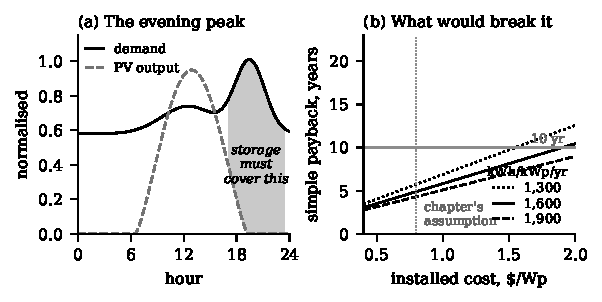
\includegraphics[width=\linewidth]{figs/solar}
\caption{(a)~Why the storage is not optional. Cuban demand peaks after sunset,
so photovoltaic capacity on its own displaces midday fuel --- the cheapest fuel
to displace --- and leaves the hours that decide whether the grid holds exactly
as they were. The load shape here is schematic; obtaining Cuba's actual hourly
demand curve is the first thing that should be done to this chapter, and
\texttt{verify.md} records it. (b)~The sensitivity the case actually turns on.
Below roughly \$1.50 per watt-peak the programme pays for itself inside a
decade across the whole plausible range of Cuban yields; above it, the argument
weakens and would need to be remade on grounds other than fuel saving.
Generated by \texttt{figs/solar.py}.}
\label{fig:solar}
\end{figure}

Here is the calculation, with its assumptions on the page so that a reader can
change them.

\begin{center}
\footnotesize
\begin{tabular}{@{}L{2.35in}r@{}}
\toprule
Target: half of a 20~TWh year from PV & 10~TWh/yr \\
Specific yield (assumed, conservative) & 1{,}600~kWh/kWp/yr \\
\midrule
Capacity required & $\approx$~6~GWp \\
Land at 1.5~ha/MWp & $\approx$~90~km$^2$ \\
\quad share of Cuban territory & $\approx$~0.08\% \\
Capital at \$0.80/Wp & $\approx$~\$5~bn \\
Evening storage, 4~h $\times$ 2~GW & 8~GWh \\
Storage at \$200/kWh & $\approx$~\$1.6~bn \\
\midrule
Total capital, over a decade & \$6--8~bn \\
Fuel displaced at 30\% efficiency & $\approx$~3~Mt/yr \\
Its value at \$400--500/t & \$1.2--1.5~bn/yr \\
\midrule
Simple payback & 5--6 years \\
\bottomrule
\end{tabular}
\end{center}

\noindent Every figure above is an order of magnitude; each is marked unverified
in the manuscript and listed in \texttt{verify.md}. Three things are
deliberately excluded and would
raise the cost: transmission and distribution reinforcement, which Cuba needs
anyway and which is a large number; the thermal fleet, which must be kept
running for firm capacity through the whole transition and therefore still needs
fuel, spares and maintenance; and the cost of capital, which for a defaulted
sovereign is the hardest input in the table and the reason
Chapter~\ref{ch:money}'s debt normalisation is a precondition rather than a
parallel exercise.

But the shape of the answer survives all of that, and the shape is the point.
The land requirement is a rounding error --- less than a tenth of one per cent
of the country, against something between one and two million hectares currently
under \emph{marab\'u} scrub. The capital cost is large but is of the same order
as a decade of the fuel bill it eliminates. And the recurring saving is in
foreign exchange, which is the scarcest thing Cuba has, converting the country's
largest recurring hard-currency cost into a domestic asset with no fuel input at
all.

That is the case, and it is a strong one. It was not a strong one in 2010, when
modules cost five times as much and batteries fifteen. The reason to do this now
is that the arithmetic changed.

\section{Hurricanes}

This is the design constraint that most solar advocacy for the Caribbean omits,
and omitting it is how a country spends five billion dollars and loses it in an
afternoon.

Cuba is hit by major hurricanes regularly and will be hit by stronger ones. The
lesson available from Puerto Rico after Mar\'ia in 2017 is specific and
usable: photovoltaic installations failed at very different rates depending on
how they were engineered, and the failures were overwhelmingly mounting failures
--- racking, fasteners, tracker stow --- rather than module failures. Systems
built to genuine high-wind specification largely survived; systems built to
mainland-United States standard specification largely did not.

\begin{design}{Building for the storm}
\label{d:storm}
\begin{rules}
\rl{1}{Specification} All installations are engineered to Category~5 wind
loading as a minimum, with mounting, fastening and foundation design certified
to that standard, and the certification published. This adds materially to
capital cost and is not optional; the alternative is to pay for the array twice.

\rl{2}{Distribution} Capacity is distributed across provinces and across many
sites rather than concentrated in a few large parks. A hurricane is a spatially
correlated risk, and the entire point of moving off a fleet of six large thermal
plants is not to rebuild that concentration in photovoltaics.

\rl{3}{Rooftops count double} Distributed rooftop generation on hospitals,
pumping stations, bakeries, telecoms sites and cold stores is resilient in a way
central capacity is not: it survives transmission damage, which is what actually
fails in a Cuban hurricane, and it keeps the critical load running while the grid
is restored.

\rl{4}{Spares held, not ordered} A national inventory of modules, inverters,
racking components and cable is held in country, in hardened storage, sized
against a modelled event. Post-storm procurement by a country with no credit
takes months.

\rl{5}{Self-insurance} Commercial insurance for Cuban assets is expensive and
in many markets unobtainable. The stabilisation fund of
Design~\ref{d:rentrule} carries an explicit reserve against grid and generation
losses, and the reserve is sized and published.
\end{rules}
\end{design}

\section{Who is allowed to own a generator}

The technology is the easy part. The reason Cuba has almost no distributed
generation despite a decade of favourable economics is legal: the national
electricity utility is a monopoly, private generation is permitted narrowly and
by permission, there is no bankable framework under which an independent producer
can sell power, and until very recently a household or private business had no
right to install a panel and use what it produced.

The solar parks now being installed with Chinese financing are the right
technology inside the wrong institution: capacity procured centrally, owned by
the state, connected to a grid the state runs, financed by a bilateral
relationship of exactly the kind Chapters~\ref{ch:sovieteconomy} and
\ref{ch:venezuela} warned about. They will help. They will not, by themselves,
solve this, and they do nothing at all about the evening peak.

\begin{design}{Generation rights}
\label{d:genrights}
\begin{rules}
\rl{1}{Rooftop by right} Any owner or lawful occupier may install generation and
storage on their own premises and consume what it produces, without permission,
subject only to published safety and interconnection standards. Not by licence,
not by category, not by application --- by right, per Design~\ref{d:commit}.2.

\rl{2}{Net billing} Surplus exported to the grid is purchased at a published
tariff set by the regulator, paid in the currency of Design~\ref{d:regime}, with
settlement periods fixed in regulation. Net \emph{billing} rather than net
metering, because the value of exported midday power is genuinely lower than the
value of consumed evening power and pretending otherwise builds a subsidy that
later has to be withdrawn.

\rl{3}{Independent producers} A standard-form power purchase agreement,
published, non-negotiable in its core terms, with international arbitration and
a payment guarantee. A one-off negotiated PPA in a country with Cuba's payment
record is not bankable; a standard instrument with a guarantee behind it can be.

\rl{4}{Regulator} An independent energy regulator with the tenure, budget and
publication obligations of Design~\ref{d:courts}, separate from the utility it
regulates and from the ministry that owns the utility. At present the operator,
the owner, the planner and the regulator are the same entity, which is the same
conflict of interest Chapter~\ref{ch:life} identifies in pharmaceuticals.

\rl{5}{Unbundling, eventually} Transmission and system operation separated from
generation, with open, non-discriminatory access to the network. This is a later
phase --- it is hard, and doing it badly is worse than not doing it --- but it
is stated here because the interconnection standards written in phase one
determine whether it is possible in phase three.

\rl{6}{Import freedom} Panels, inverters, batteries, cable and mounting hardware
enter free of duty and without licence, for anybody. Cuba currently has a
population willing to buy its own solar equipment with remittance money and a
customs regime that makes doing so an ordeal. This clause costs the state
nothing and is the single fastest megawatt available.
\end{rules}
\end{design}

\section{Biomass, and what is left of sugar}

Bagasse --- the fibre left after cane is crushed --- is the one dispatchable
renewable Cuba already knows how to burn, and the 2020 plant at Ciro Redondo
demonstrated that a modern bagasse unit can export power to the grid rather than
merely running its own mill.

The problem is that the resource has gone. Chapter~\ref{ch:crisis} recorded a
harvest in the low hundreds of thousands of tonnes; there is no bagasse because
there is no cane. So biomass in Cuba is hostage to a decision that belongs to
Chapter~\ref{ch:land}, and this chapter should not plan around a feedstock whose
existence depends on reviving an industry that mostly is not coming back.

What is available regardless is \emph{marab\'u}. The thorny scrub that has taken
over between one and two million hectares of Cuban farmland is a dense hardwood,
it already supports a small charcoal export, and clearing it serves two purposes
at once --- it recovers agricultural land and it produces fuel. It is not a
large power resource and should not be sold as one. It is a genuine transitional
one, and it is the rare case where the disposal cost of a problem is negative.

\section{The order of operations}

The last section, and the most important, because a five-billion-dollar
programme takes a decade and Cuba's problem is now.

\emph{Before anything is built.} The cheapest megawatt is the one not consumed,
and the second cheapest is the one not lost on the way. In 2023 Cuba generated
15.3 terawatt-hours and lost 3.7 of them --- close to a quarter --- in
transmission and distribution before they reached a customer.\unv{} That is an
extraordinary figure by any standard, and it means that repairing the network
delivers usable energy at a fraction of the cost per kilowatt-hour of building
new capacity to generate power that will then be lost in the same wires.

Alongside it, demand. Cuba has done this before and done it well: the 2006
programme replaced nine million incandescent bulbs and millions of inefficient
appliances and cut consumption measurably. Two decades on the appliance stock is
old again and the same intervention is available at lower cost with better
technology. Efficient lighting, refrigeration and air conditioning, industrial
motor replacement, and loss reduction are all faster, cheaper and less
capital-hungry than generation, and they can begin in month one. A programme
that goes straight to building solar parks while a quarter of the output leaks
out of the network is buying generation it will not be able to deliver.

\emph{Critical loads first.} Before utility-scale anything, put photovoltaics
and batteries on the loads whose failure is catastrophic rather than merely
expensive: hospitals, water pumping stations, cold stores, bakeries, telecoms.
These are small, fast, high-value, hurricane-resilient, and they buy the
programme public support that a distant solar park does not.

\emph{Keep the thermal fleet alive.} This is unglamorous and unavoidable. The
existing plants must provide firm capacity for the whole of the transition, which
means fuel, spares and maintenance have to be funded now, at the same time as
the new capacity is being financed. A plan that starves the old fleet to pay for
the new one produces a worse blackout in year three.

\emph{Then capacity, with storage, distributed.} Per the arithmetic above and
Designs~\ref{d:storm} and \ref{d:genrights}, over roughly a decade, with the
storage procured alongside the generation and not after it.

\begin{design}{The energy sequence}
\label{d:energyseq}
\begin{rules}
\rl{1}{Months 0--6} Import liberalisation for equipment (Design~\ref{d:genrights}.6);
rooftop rights by decree; efficiency programme launched; critical-load
installations begun; fuel and spares for the existing fleet funded as a first
call on the budget.

\rl{2}{Months 6--24} Regulator established; standard PPA published; net billing
tariff set; interconnection standards issued; first independent producer
tenders, competitively bid with published results per
Chapter~\ref{ch:integrity}.

\rl{3}{Years 2--10} Roughly 6~GWp and 8~GWh built out, distributed across
provinces, with the eastern provinces weighted first --- they have the worst
supply, the most land and the least political voice, and per
Design~\ref{d:municipal}.2 the design does not let the benefits accrue where the
tourists are.

\rl{4}{Throughout} No preferential allocation of capacity, fuel, currency or
grid access to any state or military-linked entity. Energy is where Cuban
discretion has been most valuable and therefore most corrupting, and
Chapter~\ref{ch:integrity} treats generation procurement as a priority
publication target.
\end{rules}
\end{design}

\chapter{Visitors}
\label{ch:tourism}

\section{The industry Cuba built, and what it cost}

Cuba rebuilt tourism from almost nothing after 1990 --- 340,000 visitors in that
year, 4.7 million in 2018 --- and by any conventional measure that is a success.
The trouble is what happened next, and it is the clearest case study in this book
of investment allocated by power rather than by return.

Through the decade to 2024 the Cuban state, principally through the
military-linked conglomerate GAESA and its hotel arm, built hotel rooms at a
sustained and increasing rate while occupancy collapsed.

The 2024 figures are worth setting out in full, and in shares rather than in
pesos, because shares are immune to the exchange-rate problem of the note on
sources. Of total national investment that year, business services, real estate
and rentals took 24.9 billion pesos and hotels and restaurants a further 11.9
billion --- together 37.4 per cent of everything the country invested.
Agriculture, livestock and forestry took 2.6 billion, or 2.7 per cent. Public
health and social assistance took 2.0 billion, less than a fifth of what went
into hotels and restaurants alone. As the economist Pedro Monreal put it,
agricultural investment was fourteen times smaller than tourism's
\citep{oneiinv}.\unv{}

That is the allocation of a country importing most of its food, unable to light
its cities, appealing to the World Food Programme for children's milk, and
running its existing hotels at occupancy rates reported around a quarter. New
hotels opened into a market with no guests while the pumping stations that
supply those same hotels with water failed for want of parts.

No market signal produced that, and no market signal could have. It was
produced by an institution that could
allocate capital to itself, without publishing a return, without competing for
the funds, and without anyone in a position to say no. Chapter~\ref{ch:integrity}
uses this as its worked example, because it demonstrates that Cuba's investment
problem is not primarily a shortage of capital. It is that the capital which
exists is allocated by whoever controls it, to whatever they control.

Two other features of the industry as built matter for what follows.

It was an \emph{enclave}. The dominant form is the all-inclusive beach resort at
Varadero and the northern cays, physically separated from the country around it,
supplied largely with imported food, staffed by workers paid in pesos through a
state agency that keeps the currency spread, and --- until 2008 --- legally
closed to Cubans. The Caribbean-wide evidence on this model is that the share of
the visitor's spending which stays in the host country is low, commonly cited in
the range of a fifth to a third for all-inclusives, with the remainder accruing
to the foreign tour operator, the foreign airline and the imported supply
chain.\unv{} Cuba adopted the model that leaks most.

And it carries a memory. Chapter~\ref{ch:inheritance} described the Havana of
the 1950s: casinos, organised crime, a pleasure district for foreigners in a
country whose own people were excluded. The revolution's founding claim included
abolishing that. Any proposal to make tourism an anchor industry has to answer
the objection that it recreates it, and the answer cannot be that times have
changed. It has to be a design in which Cubans own the businesses, are not
excluded from the spaces, and capture the income.

\section{The strategy: value per visitor, not visitors}

The book proposes an explicit reversal of the metric the industry has been run
on.

Cuba should not pursue arrival numbers. It should pursue \emph{net foreign
exchange retained per visitor}, and should be willing to accept fewer visitors
to raise it.

The reasoning is partly environmental and partly arithmetic. Chapter~\ref{ch:nature}
sets out what mass tourism does to reefs, wetlands and colonial fabric, and Cuba's
comparative advantage is precisely the thing that volume destroys. But the
arithmetic is sufficient on its own: a visitor in a private room eating in
private restaurants and buying from private guides leaves several times as much
in Cuban hands as a visitor in an all-inclusive, even when the second one paid
more for the holiday. On a labour-constrained island with a failing grid, adding
visitors is expensive --- each one needs water, power, food and staff, all of
which are scarce --- while adding value per visitor is nearly free.

This also resolves the tension with Chapter~\ref{ch:premises}'s labour
constraint. Cuba does not have the people for a Cancún. It does have the people
for something better paid.

\begin{design}{The visitor economy}
\label{d:visitor}
\begin{rules}
\rl{1}{The metric} The published objective of tourism policy is net foreign
exchange retained per visitor-night, reported annually with its components. No
arrival target is set or published. What a state measures is what it builds, and
Cuba built rooms because it counted arrivals.

\rl{2}{Private by default} Accommodation, food service, guiding, transport and
retail to visitors are open to private and cooperative providers by right, under
Design~\ref{d:commit}.2, with the state's role confined to standards, safety and
inspection. The \emph{casa particular} and the \emph{paladar} are the default
form of the Cuban tourism industry, not its tolerated margin.

\rl{3}{Direct employment and direct payment} The state employment agency
arrangement is abolished for this sector as for all others
(Chapter~\ref{ch:capital}): hotels hire their own staff and pay them directly.
The currency spread taken from tourism workers is the industry's founding
injustice and it is also why the service is indifferent.

\rl{4}{Local procurement} Accommodation businesses above a size threshold must
publish the share of food purchased domestically, and the accommodation levy of
Design~\ref{d:tax}.7 is set at two rates, the lower applying above a published
domestic-procurement threshold. This is the instrument that connects
Chapter~\ref{ch:land} to this chapter: Cuban agriculture's most reliable
potential customer is standing in a hotel two hours away, buying imported
tomatoes.

\rl{5}{No new state hotels} A moratorium on state hotel construction until
system-wide occupancy exceeds a published threshold for two consecutive years.
The capital released is redirected under Chapter~\ref{ch:sequence}'s financing
table. This is the single largest reallocation of investment available to Cuba
and it requires no foreign money at all.

\rl{6}{Open to Cubans} No facility, beach, cay or district is closed to Cuban
residents, in law or in practice, and the prohibition is justiciable under
Design~\ref{d:courts}.4.
\end{rules}
\end{design}

\section{What Cuba actually has}

The asset is not beach. Every country in the Caribbean has beach, several have
better, and competing on it means competing on price with places that have
better airports and working electricity.

What Cuba has that the competition does not is a combination that cannot be
built: nine UNESCO World Heritage sites; four intact colonial cities; a musical
culture that is a destination in itself; some of the best-preserved coral in the
hemisphere at the Jardines de la Reina; the largest wetland in the insular
Caribbean at Zapata, with the endemic bird list that goes with it; five thousand
seven hundred kilometres of coast, much of it undeveloped; and --- unusually and
importantly --- a very low violent crime rate, which is a decisive advantage in a
region where several competitors have the opposite reputation.

The products that follow from that list are diving, birding and nature tourism,
cultural and musical tourism, architectural and heritage tourism, medical
tourism under Chapter~\ref{ch:life}, and long-stay visitors under
Chapter~\ref{ch:talent} --- all of which are higher-value, lower-volume, less
seasonal and less environmentally destructive than beach resorts, and all of
which are currently underdeveloped or absent.

\subsection{The Old Havana precedent}

Cuba has already built the best heritage institution in the Caribbean and then
dismantled it, and the episode is instructive in both directions.

The Office of the City Historian of Havana, under Eusebio Leal, was given in 1993
something no other Cuban body had: the right to run commercial enterprises in
Old Havana --- hotels, restaurants, shops --- and to \emph{retain and reinvest its
own revenue} in restoring the district. It worked. Old Havana's restoration is
the most successful physical project of the Cuban period, it was self-financing,
it employed and trained local residents, it restored housing alongside monuments
rather than displacing people, and it produced a district that is now the single
strongest tourism asset in the country.

In 2016 its commercial arm was transferred to the military conglomerate, and the
Office's independent revenue base with it.

Both halves belong in the design. The mechanism --- a heritage authority that
keeps its own earnings and is accountable for the fabric --- is correct and
should be extended to Trinidad, Cienfuegos, Camag\"uey and Santiago. And the
reversal is the reason it has to be entrenched under Design~\ref{d:commit}
rather than granted, because it was granted, it worked for twenty-three years,
and it was taken away.

\begin{design}{Heritage authorities}
\label{d:heritage}
\begin{rules}
\rl{1}{Form} A statutory heritage authority for each historic city, with
jurisdiction over planning consent, building standards and public space in its
district.

\rl{2}{Revenue} It retains a defined share of the accommodation levy and of
concession income raised in its district, by statute and not by grant, and this
share may be altered only by legislation.

\rl{3}{Obligation} A published, audited restoration programme, and a binding
requirement that a fixed share of restored floorspace remains residential and
that existing residents have a right to rehousing within the district. Heritage
tourism that empties a district of its inhabitants produces a stage set and
loses the thing visitors came for.

\rl{4}{Independence} Its commercial arm may not be transferred to any other
entity without legislation. Written because this is exactly what happened.
\end{rules}
\end{design}

\section{Carrying capacity}

Chapter~\ref{ch:nature} makes the environmental argument at length. What belongs
here is that it is an economic argument, not a sentimental one.

The Cuban reefs, the Zapata wetland and the cays are the physical stock that the
high-value products above are sold from. A reef that is bleached, dynamited by
anchors or silted by coastal construction stops producing revenue permanently,
and the revenue it was producing was the highest per visitor in the industry.
Diving tourism at the Jardines de la Reina works precisely because the fishing
was excluded and the sharks are still there; it is worth more per visitor-day
than any beach resort in the country and it exists only because someone drew a
line on a map and enforced it.

\begin{design}{Limits}
\label{d:limits}
\begin{rules}
\rl{1}{Site limits} Published daily and annual visitor limits for reef, cay and
protected-area sites, set by the environmental regulator of
Chapter~\ref{ch:nature} and not by the tourism ministry, with access allocated by
published auction or ballot rather than by administrative permission.

\rl{2}{Coastal setback} A statutory construction setback from the shoreline,
applied without exception, including to existing state and military-linked
operators. Chapter~\ref{ch:nature} sets the distance; this clause is about the
absence of exceptions, which is where every Caribbean setback rule has failed.

\rl{3}{No new cay causeways} The \emph{pedraplenes} that connect the northern
cays to the mainland have measurably damaged water circulation and the
ecosystems behind them. No further ones are built, and remediation of the
existing ones is assessed.

\rl{4}{Price the scarcity} Where a site is at its limit, the access price rises.
This is the mechanism that converts an environmental constraint into revenue
under Design~\ref{d:visitor}.1 rather than into a queue.
\end{rules}
\end{design}

\section{Dutch disease, and the wage problem}

A successful tourism sector earning foreign exchange will, under
Chapter~\ref{ch:money}'s dollarised regime, raise domestic prices and wages in
the sectors that serve it and squeeze everything that competes with imports ---
which is agriculture, which is the sector Chapter~\ref{ch:land} needs to grow.
This is the standard resource-boom pathology and it is aggravated here by the
labour constraint: there is no reserve of workers to expand into the boom
sector, so it draws them from the others.

Cuba has already run this experiment. In the 1990s the tourism wage drew doctors
into taxi driving and surgeons into renting rooms, which is where the inverted
pyramid of Chapter~\ref{ch:dollarreform} came from.

\begin{design}{Not repeating the 1990s}
\label{d:dutch}
\begin{rules}
\rl{1}{Public pay is the control} Design~\ref{d:pay} binds here. Public
professional pay is benchmarked against the tourism and private wage and moves
with it. A tourism strategy adopted without the corresponding public pay
settlement is a strategy for emptying the hospitals, and this book will not
propose one.

\rl{2}{Revenue to the fund} The accommodation levy and concession revenue are
rent under Design~\ref{d:rentrule} and go to the stabilisation and investment
fund, not to the recurrent budget --- which both dampens the domestic demand
impulse and stops a tourism boom from financing recurrent commitments that a
bust cannot sustain.

\rl{3}{Linkage over expansion} Policy effort goes into raising the domestic
content of each visitor's spending --- food, furniture, textiles, crafts, guiding
--- rather than into raising visitor numbers. Linkage is the instrument that
turns a boom sector into a diversified one, and it is the reason
Design~\ref{d:visitor}.4 is written as a tax differential rather than as an
exhortation.

\rl{4}{Regional weighting} Tourism development incentives are weighted toward
the eastern provinces, per Design~\ref{d:municipal}.2. Left alone, the industry
concentrates in Havana, Varadero and the northern cays, and the equalisation
formula then has to do all the work.
\end{rules}
\end{design}

\chapter{The second track}
\label{ch:talent}

\section{The claim, stated carefully}

This is the most speculative chapter in the book and it should announce that
before it argues anything.

The claim is that Cuba can build a second export sector, alongside tourism, out
of educated people selling services across a border without leaving the island
--- software, engineering, design, back-office work, data work, Spanish-language
content, remote professional services --- and that this sector could plausibly
reach the same order of magnitude as tourism within a decade.

The claim is not that Cuba becomes an artificial-intelligence power. It will not.
Training large models requires electricity Cuba does not have, capital it cannot
raise, and hardware it cannot legally buy. Any proposal that has Cuba building
data centres is not a proposal about Cuba. What Cuba can plausibly do is supply
\emph{labour} into the global services market that the current technology wave
has expanded --- the annotation, evaluation, localisation, integration, tooling
and ordinary software engineering that sit around the models rather than inside
them --- and it can do so in Spanish, in the New York time zone, with a
workforce that can read.

The arithmetic is worth putting on the page because it is the reason the chapter
exists. A hundred thousand Cubans --- about two per cent of the labour force ---
earning an average of eighteen thousand dollars a year in remote services would
generate roughly \$1.8 billion annually in foreign exchange.\unv{} That is the
same order as Cuban tourism earnings in a good year, from a sector requiring no
hotels, no beach, no water supply, no fuel and almost no capital. The per-worker
figure is well below what a comparable worker earns in a high-income country and
well above anything available in Cuba today, which is precisely why the market
would clear.

\section{Why it has not happened}

Cuba has had educated, underemployed, English-capable technical workers for
thirty years, and the global market for remote services has existed for twenty.
The sector did not appear. The reasons are specific, and identifying the binding
one is the whole content of this chapter.

It is not talent. Cuban technical education is the asset Chapter~\ref{ch:socialstate}
described, and Cuban programmers working abroad are competitive.

It is not, primarily, the embargo. American clients are constrained, but Spain,
Mexico, Argentina, Canada, Germany and the entire Spanish-speaking world are
not, and none of them buys Cuban services at scale either.

It is not, mainly, connectivity --- though connectivity is a real constraint and
the next section is about it. Plenty of countries export services on worse
bandwidth than Havana has had since 2018.

\emph{The binding constraint is that a Cuban cannot lawfully and reliably
contract with a foreign client and be paid into an account they control.} Until
2021 a Cuban private operator had no legal personality and so could not sign a
contract as an entity. The permitted-activity list was written in the vocabulary
of trades and had no category for a software developer or a design studio.
Foreign-currency accounts were restricted. International card and transfer rails
did not reach individuals. And professionals trained at state expense were, for
much of the period, prohibited from practising their profession privately at all.

The result is that Cubans who do this work do it informally, through a relative's
foreign account, or through an intermediary in Miami or Madrid who takes a cut
and holds the client relationship --- or, increasingly, they emigrate, which
converts a potential export sector into a permanent loss.

This is the good news in the chapter. The binding constraint is legal, it is
domestic, it costs the state nothing to remove, and it does not require anyone's
permission.

\begin{design}{The right to sell your own work}
\label{d:contract}
\begin{rules}
\rl{1}{The core right} Any resident may contract directly with a foreign client,
in any currency, without licence, intermediary or prior authorisation, and may
receive payment into an account in their own name and spend from it. This is the
single most important clause in Part~III's growth strategy and it is a repeal,
not a programme.

\rl{2}{Professions included} Explicitly extended to professions trained at state
expense --- engineers, physicians, architects, lawyers, scientists. The exclusion
of professionals from self-employment since 1993 is the reason Cuba's private
sector is a collection of trades, and it is the reason its most valuable workers
had only two options, the state or the airport.

\rl{3}{No enumerated list} Per Design~\ref{d:commit}.2, service exports are
permitted by right. Any list of permitted activities in this domain would be
obsolete before it was published, which is a general argument against lists and a
decisive one here.

\rl{4}{A simple tax that is worth paying} Income from cross-border services pays
the low flat rate of Design~\ref{d:tax}.6, filed annually, with no deductions and
no separate social contribution. A mobile base taxed heavily is not taxed; a
mobile base taxed lightly and simply is registered, counted, and eventually
becomes a constituency for the system that registered it.

\rl{5}{Equipment} Computers, phones, networking hardware and their parts enter
free of duty and licence, per Design~\ref{d:genrights}.6. Cuba currently has
citizens buying their own tools with remittance money and a customs regime that
treats it as smuggling.

\rl{6}{Classification} Cross-border services are classified and counted as
exports in the national accounts and the balance of payments, which sounds
clerical and is not: what is not measured is not defended in the budget, and this
sector will need defending against the ministries whose staff it draws.
\end{rules}
\end{design}

\section{Connectivity}

Cuba came online late and expensively. Mobile data arrived in December 2018;
international capacity has run principally through a single submarine cable laid
from Venezuela in 2011, which is both a bandwidth constraint and a single point
of failure; the state telecommunications company is a monopoly; and the price of
data as a share of Cuban income has been among the highest in the world, which is
what the protests over the 2025 tariff changes were about.

No second track exists on that basis. A foreign client contracting with a Cuban
supplier is buying reliability, and reliability is exactly what a single cable, a
monopoly operator, a fragile grid and a state that switched off mobile data
nationally on 11 July 2021 do not provide.

\begin{design}{Connectivity as infrastructure}
\label{d:connect}
\begin{rules}
\rl{1}{Redundancy} At least two additional international routes, on diverse
physical paths and diverse landing points, procured on published competitive
terms. One cable is not a network.

\rl{2}{Open wholesale access} Whatever the ownership of the international and
backbone capacity, access to it is sold to any licensed retail provider on
published, non-discriminatory terms, regulated by an independent authority on
the model of Design~\ref{d:genrights}.4. Retail competition is what moves the
price; full privatisation of the incumbent is not required and should not be
attempted early.

\rl{3}{No political interruption} Per Design~\ref{d:minimum}.5. This is
restated here because it is a commercial clause as much as a civil-liberties
one: a country whose government has demonstrated that it will switch off the
internet during a political event cannot sell service-level agreements, and
every potential client knows it.

\rl{4}{Price transparency} Published wholesale and retail tariffs, and a
published affordability metric --- data cost as a share of median income ---
reported annually.

\rl{5}{Power} Telecommunications sites are critical loads under
Design~\ref{d:energyseq}.1 and are among the first to receive photovoltaics and
storage. A network that goes down with the grid is not a network either.
\end{rules}
\end{design}

\section{The residence regime}

Only after the two designs above does a visa policy make any sense, and the
ordering matters because the international discussion of this subject has it
backwards.

The digital-nomad visa is a modest instrument. The honest reading of the
international experience --- Estonia, Portugal, Barbados, Croatia, Costa Rica ---
is that these schemes attract a few thousand people, generate useful but small
consumption spending, and do not by themselves build an industry. Barbados's
Welcome Stamp was a competent response to a pandemic-era collapse in tourism, not
an economic transformation. Estonia's e-Residency, the most cited of them, has
enrolled a large number of people and produced a much smaller number of real
businesses paying real Estonian tax.

What actually built service exports in the comparator countries was not visas for
foreigners. It was \emph{residents being allowed and able to sell their work
abroad}, plus predictable law and a payment system --- which is
Design~\ref{d:contract}. Uruguay's software export sector, the most relevant Latin
American case, was built on domestic firms and domestic engineers, not on
inbound nomads.

So the residence regime here is proposed for three narrower and more defensible
reasons: it brings in people who train and hire locally; it brings in demand for
the long-stay accommodation that Chapter~\ref{ch:tourism} wants to grow instead
of hotel rooms; and --- per Design~\ref{d:pension}.3 --- more working-age
residents is the cheapest available instrument for a dependency ratio.

\begin{design}{Residence for mobile workers}
\label{d:residence}
\begin{rules}
\rl{1}{The permit} A renewable residence permit for a person with foreign income
from remote work or a foreign business, granted on published objective criteria
--- income threshold, health cover, clean record --- with a statutory decision
period and deemed grant if the period passes. No discretion, no interview, no
sponsor.

\rl{2}{Tax certainty} A published flat rate on locally-remitted income for a
fixed number of years, legislated rather than administered, with the treatment
of foreign income stated in advance. Uncertainty deters this population far more
than rates do.

\rl{3}{Ordinary rights} The right to rent, to open an account, to import personal
equipment, to bring family, and to use the health system on the same terms as
residents while paying the same taxes. A permit that does not allow a bank
account is not a permit.

\rl{4}{A route to staying} A defined path to permanent residence and, for those
who want it, naturalisation. The objective is residents, not visitors; a scheme
that resets every year selects for people who do not put down roots.

\rl{5}{Local linkage} A reduced rate for permit-holders who employ or formally
train Cuban residents, verified simply and audited. This is what converts an
inbound flow into a domestic industry, and it is the difference between this
proposal and a beach with better wifi.
\end{rules}
\end{design}

\section{The diaspora, and not taxing the door}

Two million people abroad, most of them one flight away, many with capital and
professional standing, and a substantial number who would work with Cuba if
working with Cuba were possible. They are simultaneously the natural first
clients for this sector, the natural first investors under
Chapter~\ref{ch:capital}, and the largest single reservoir of the working-age
people Chapter~\ref{ch:premises} says the country has lost.

\begin{design}{Circulation, not retention}
\label{d:diaspora}
\begin{rules}
\rl{1}{No exit tax} Cuba does not tax, fine, or impose a training levy on
emigrants. The instrument is popular with governments losing skilled workers, it
collects almost nothing, it is trivially avoided by simply not returning, and it
converts a temporary departure into a permanent one. It is also, in Cuba
specifically, a tax on the grievance this book is trying to settle.

\rl{2}{Return without penalty} Full restoration of residence, property rights,
professional registration and pension entitlement for returning Cubans,
automatic and without discretionary review, including for those who left
irregularly or abandoned a mission.

\rl{3}{Dual nationality} Recognised, with the right to hold property, to invest,
to work, to vote in local elections after a residence qualification, and to
inherit. Chapter~\ref{ch:capital} depends on this; so does the pension
portability of Design~\ref{d:pension}.4.

\rl{4}{Voluntary contribution} Cubans abroad may contribute voluntarily to the
Cuban social insurance system and accrue entitlement, per
Design~\ref{d:pension}.4. This converts a diaspora into a contributor base,
which no other instrument does.

\rl{5}{Faculty and clients} Programmes to bring diaspora academics and
professionals back on short teaching, clinical and advisory terms, with no
political test, administered by universities rather than by ministries.
\end{rules}
\end{design}

\section{The universities}

The sector proposed here needs a pipeline, and Chapter~\ref{ch:socialstate}
identified the specific gap: Cuba produces excellent engineers, physicians and
mathematicians and very few people trained in the disciplines an institutional
transition and a services economy actually run on --- commercial law, accounting,
finance, management, applied economics, and the empirical social sciences.

\begin{design}{Academic capacity}
\label{d:university}
\begin{rules}
\rl{1}{Autonomy} Universities appoint their own staff, set their own curricula
and admit their own students on published academic criteria. Political record is
not an admission or appointment criterion, and the prohibition is justiciable.

\rl{2}{The missing disciplines} A funded programme to build law, accounting,
finance, management and applied economics faculties, with foreign partnership,
visiting appointments from the diaspora, and professional accreditation
recognised internationally. This is a decade-long constraint on everything in
Part~III --- Design~\ref{d:courts}.6 needs commercial judges, and
Chapter~\ref{ch:welfare} needs tax administrators --- and it binds from year one.

\rl{3}{Foreign partnership} Joint programmes, dual degrees and branch
arrangements with foreign universities, permitted by right and regulated for
quality only.

\rl{4}{Publish and be read} Cuban academic work published openly, and Cuban
academics free to publish abroad, collaborate and travel. The dismantling of the
Centre for the Study of the Americas in 1996 taught Cuban social science what
happens to research that analyses policy, and that lesson has to be publicly
unlearned before anyone will do the work this book's later phases need.
\end{rules}
\end{design}

\section{What this chapter cannot promise}

Three honest limits.

The sector is small until the electricity is fixed. Everything here is downstream
of Chapter~\ref{ch:energy}, and a remote worker in a province with sixteen-hour
blackouts cannot take a call.

The sector competes for exactly the people the state most needs. Every engineer
who moves to remote work at eighteen thousand dollars a year is an engineer not
in the ministry, the utility or the university at a state wage --- which is why
Design~\ref{d:pay} is a precondition for this chapter and not a separate topic.

And the sector is a rival to emigration, not a complement to it. Its real
justification is that it offers a person the income they left for without
requiring them to leave. If it works, the outflow slows; if the outflow does not
slow, it is not working, and Chapter~\ref{ch:sequence} makes net migration one of
the indicators by which this book can be judged to be failing.

\chapter{Life sciences}
\label{ch:life}

\section{The one sector that already owns something}

Everywhere else in Part III the problem is building a capability. Here the
capability exists, is forty years old, has products, has a reputation, and has
never been organised to sell anything.

Cuban biotechnology began in the early 1980s as a deliberate state decision to
build a research capacity in a poor country, and it produced, against every
reasonable expectation, a genuine one. The institutions --- the Centre for
Genetic Engineering and Biotechnology, the Finlay Institute, the Centre of
Molecular Immunology, and the rest, consolidated since 2012 into the
BioCubaFarma holding --- have delivered products that were not derivative.

The meningococcal B vaccine developed at the Finlay Institute in the 1980s was
the first of its kind anywhere. The \emph{Haemophilus influenzae} type b vaccine
licensed in 2004 used a fully synthetic antigen, the first synthetic-antigen
vaccine in routine human use. Heberprot-P, a recombinant epidermal growth factor
injected into diabetic foot ulcers, addresses a condition that causes a large
number of the world's amputations and has no close equivalent elsewhere.
CIMAvax-EGF, a therapeutic lung cancer vaccine, has been sufficiently interesting
to American oncologists that a United States cancer centre pursued trials of it
through the licensing exceptions. And in 2021 the sector developed, tested,
manufactured and deployed its own COVID-19 vaccines, vaccinating over ninety per
cent of the population --- the only country in Latin America to do so, and it did
it while unable to reliably import syringes.\unv{}

Why did this work when nothing else did? Three reasons, and they are worth
naming because the reform must not destroy them.

It was a \emph{closed loop}. Research, clinical development, manufacture and
deployment sat inside one system with one customer, the national health service,
so a product went from bench to population without an intervening market and
without a reimbursement negotiation. That is a genuine structural advantage for
developing products aimed at a whole population.

It had \emph{patient capital}. The state funded it for a decade before results,
which no shareholder would have done, and did not close it during the Special
Period.

And it had \emph{no profit constraint on target selection}. It worked on
meningitis B, on diabetic foot, on lung cancer in smokers --- conditions of
interest to Cuba and to poor countries generally rather than to the markets that
set global pharmaceutical priorities.

\section{Why it earns almost nothing}

And yet. Cuban pharmaceutical and biotechnology exports are, by any published
measure, a small fraction of what a portfolio like this should be worth --- of
the order of a few hundred million dollars a year, against a global market in the
trillions and against Cuban medical \emph{services} exports that were at their
peak twenty or thirty times larger.\unv{}

The reasons are not scientific. They are regulatory, contractual and financial,
and each is fixable.

\emph{No regulatory conversion.} Almost nothing in the portfolio holds approval
from the United States Food and Drug Administration or the European Medicines
Agency, and much of the clinical evidence was not generated to the standards
those agencies require --- not because the trials were dishonest, but because
they were designed for Cuban registration and published in Cuban journals. A
product without a stringent-authority approval cannot be sold in the markets that
pay, cannot be licensed to a partner who sells there, and cannot be priced at
anything like its therapeutic value. The COVID vaccines are the clearest case:
Cuba developed vaccines that worked, and could not sell them, because they did
not complete the international prequalification pathway.

\emph{No distribution partner.} Value in pharmaceuticals is captured through
regulatory affairs, distribution, salesforce and reimbursement negotiation ---
capabilities Cuba does not have and would take twenty years to build. The answer
is to partner, and Cuba has largely not partnered, in part because of the next
two reasons.

\emph{No capital.} Bringing one product through international trials costs more
than the whole sector's annual budget, and a defaulted sovereign cannot finance
it.

\emph{An ownership structure nobody will contract with.} A foreign
pharmaceutical company entering a licensing deal is buying a stream of
obligations enforceable over fifteen years. Its counterparty in Cuba is a state
holding company, in a jurisdiction with no independent courts, subject to a
statute that exposes anyone trafficking in confiscated property to litigation in
the United States, with a sovereign that froze foreign firms' accounts in 2009.
The science is not the risk.

\emph{And the regulator is the producer.} The Cuban medicines regulator, CECMED,
is a state body regulating products made by state bodies, within a single system
answerable to one government. Whatever the integrity of its individual staff ---
and its technical reputation is not bad --- it is structurally not independent,
and structural independence is precisely what a foreign regulator or a foreign
partner is looking for. This is the same conflict of interest
Chapter~\ref{ch:energy} identified in electricity, where the operator, owner,
planner and regulator are one entity.

\section{The design}

The strategy is to convert an existing scientific asset into an investable,
regulated, exporting sector without destroying the closed loop that made it work.
The order matters: regulator first, because nothing else is possible until a
foreign counterparty can rely on something.

\begin{design}{An independent medicines regulator}
\label{d:cecmed}
\begin{rules}
\rl{1}{Separation} The medicines regulator is constituted as an independent
authority with the tenure, budget and publication guarantees of
Design~\ref{d:courts}, institutionally separate from BioCubaFarma, from the
health ministry as owner, and from any producing entity.

\rl{2}{Fee-funded and published} Funded by application fees at published rates,
with all assessment reports, approvals, refusals and inspection findings
published, as the European and American agencies publish theirs. Publication is
what makes a regulator's judgments checkable by outsiders, which is the entire
asset being built.

\rl{3}{Target: stringent-authority status} An explicit, dated programme to reach
World Health Organization listed-authority standing, with the assessment
criteria, the gap analysis and the progress published annually. This is a
multi-year technical project with a definite endpoint, and it is the single
highest-return institutional investment available to Cuba in any sector.

\rl{4}{Reliance in the interim} Automatic recognition of approvals by stringent
foreign regulators for products Cuba imports, so that scarce assessor capacity is
spent on Cuban products seeking export rather than on re-reviewing medicines
already approved elsewhere. This also, immediately, shortens the queue for
imported medicines that are currently absent from pharmacies.

\rl{5}{Trials to international standard} All Cuban clinical trials conducted and
registered to international good-clinical-practice standards, in international
registries, with independent monitoring and ethics review. Cuban trial data is
currently discounted abroad for reasons of procedure rather than of substance,
and this clause is what makes forty years of accumulated science sellable.
\end{rules}
\end{design}

\begin{design}{Capital and partnership}
\label{d:biopartner}
\begin{rules}
\rl{1}{Product-level joint ventures} Partnership at the level of the individual
product --- one asset, one partner, defined territories, defined milestones ---
rather than at the level of the institution. This raises capital and buys
regulatory and distribution capability without selling the research base.

\rl{2}{Keep the platform, license the product} Cuba retains ownership of its
research institutions, its manufacturing and its underlying technology
platforms, and licenses rights to specific products in specific markets. The
comparators are Singapore and Ireland --- countries that built pharmaceutical
sectors by hosting and partnering rather than by originating --- and not
Switzerland, which is not an available model for a country of nine million with
no capital.

\rl{3}{Enforceable terms} Contracts under foreign law with international
arbitration, per Chapter~\ref{ch:capital}. A licensing agreement justiciable
only in Cuban courts is worth a fraction of the same agreement justiciable in
London or Singapore, and the discount is larger than anything Cuba could
negotiate on the royalty.

\rl{4}{Diaspora scientists} Cuban scientists abroad are the natural bridge to
foreign partners, regulators and capital, and Design~\ref{d:diaspora}.5 applies
directly. Several of the people best placed to take a Cuban product through an
FDA submission are Cubans who left.

\rl{5}{The domestic supply first} Nothing in this design permits export of a
medicine that is unavailable in Cuban pharmacies. Domestic supply is the first
call on production, stated as a rule because the revenue pressure will run the
other way.
\end{rules}
\end{design}

\section{The medical missions, reformed}

Cuba's largest export for over a decade was the labour of its health workers, and
Chapter~\ref{ch:venezuela} reported both halves of that: a real service really
delivered in places no other country would staff, financed by paying the workers
a fraction of the contract value and, in several destinations, holding their
passports.

The programme should be kept. It is valuable, it is genuinely good for the
receiving countries, and it is one of the few things Cuba sells that nobody else
sells. But the labour arrangement has to change, and the argument for changing it
is not only ethical. It is that the industry's binding constraint is now the
supply of willing doctors --- Cuban health workers are leaving the country
altogether, and a programme that treats them as conscripts loses them to
emigration, which yields Cuba nothing at all.

\begin{design}{Medical service export}
\label{d:missions}
\begin{rules}
\rl{1}{Individual contracts} Each health worker contracts individually, with the
full contract value disclosed to them and a published minimum share payable to
the worker. The state may retain a share --- there is a legitimate public claim on
the return to a publicly funded training --- and the share is published,
legislated, and the same for everyone.

\rl{2}{No control of documents or movement} Passports are held by their owners.
Restrictions on residence, association and relationships are abolished. The
penalty for leaving a mission is contractual, not a bar on returning to one's
own country, and Design~\ref{d:diaspora}.2 applies.

\rl{3}{Voluntary} Participation is voluntary, refusal carries no professional
consequence, and this is auditable.

\rl{4}{Compliant with labour standards} The programme is brought into conformity
with international labour conventions, and the conformity is externally verified
and published. This is what converts a programme under permanent international
criticism into an exportable, expandable and defensible service.

\rl{5}{Domestic staffing floor} A published minimum staffing level for the Cuban
health service, below which missions are not staffed. Per
Chapter~\ref{ch:premises}, people are the binding scarcity, and the domestic
system is the asset the whole book is written to protect.
\end{rules}
\end{design}

\section{Two further lines of business}

\emph{Clinical trials as an export.} Cuba has attributes that contract research
organisations pay for: a population with universal health coverage and complete
medical records, high follow-up and retention because people do not move or lose
their insurance, a physician-dense primary care network organised by defined
population, and a trial cost base far below North America or Europe. Under
Design~\ref{d:cecmed}.5 and an independent ethics framework, running phases of
international trials in Cuba is a genuine, capital-light, high-skill export that
also brings the domestic system access to investigational treatments. It requires
scrupulous consent standards --- a population that has limited access to medicines
is a population that can be induced to enrol --- and the ethics review has to be
independent of both the sponsor and the state, which is a stronger requirement
than most middle-income trial hosts apply.

\emph{Health tourism.} Cuba has treated foreign patients for decades and could
do far more of it, in cardiology, orthopaedics, ophthalmology, oncology,
neurological rehabilitation and addiction treatment, at prices well below the
United States and with outcomes that stand comparison. The constraint is
Chapter~\ref{ch:premises}'s again: every foreign patient consumes a Cuban
clinician's time. Design~\ref{d:delivery}.3 already binds --- designated
facilities, ring-fenced staff, revenue to the public system, and the programme
stops if the ring-fence cannot be held. This chapter adds nothing to that except
the observation that health tourism is the most valuable visitor per bed-night
available under Chapter~\ref{ch:tourism}'s metric, and the least environmentally
damaging.

\section{What is being protected}

A closing caution, because the reforms above are all in the direction of markets
and partnership and that direction has a known failure mode.

The Cuban biotechnology sector works because it is a closed loop with a public
customer, patient capital and no obligation to select targets by market size. Open
it to partnership incorrectly and it becomes a contract manufacturer for
somebody else's pipeline, with its research agenda set in New Jersey and its
public-health function abandoned --- at which point Cuba has sold its one
originating capability for a manufacturing margin.

The clauses that guard against that are Design~\ref{d:biopartner}.2, which keeps
the platform and licenses only products; Design~\ref{d:biopartner}.5, which puts
the domestic pharmacy first; and the public research budget, which
Chapter~\ref{ch:welfare}'s floor protects. They are the whole of the protection,
they are not self-enforcing, and a future government under fiscal pressure will
be offered a great deal of money to weaken them.

\chapter{Land and food}
\label{ch:land}

\section{The failure, stated exactly}

A tropical island with deep soils, adequate rainfall, a year-round growing
season, no frost, a trained agronomic profession and a hundred and fifty years of
commercial agriculture imports somewhere between two thirds and four fifths of
what it eats, cannot pay for the imports, and has between one and two million
hectares of farmland under \emph{marab\'u} scrub.\unv{}

This is the most complete policy failure in the book. It is more complete than
the energy failure, because energy at least has a physical explanation --- the
plants are old and the fuel is foreign. Nothing physical explains this one. Cuba's
neighbours with worse soil, worse rainfall and less education feed themselves.

It is also the clearest case where the embargo explains very little. Cuba may buy
agricultural inputs from anyone in the world, and does buy food from the United
States itself, for cash, under the exemption that has stood since 2000. The
constraint is not permission to import fertiliser. It is that Cuban farmers have
been given every incentive not to grow anything.

\section{Why}

Four mechanisms, in order of how much they explain.

\emph{Acopio.} The state procurement monopoly requires producers to sell a
defined share of output to the state at a state-set price, historically below the
cost of production and paid late, in a currency that was losing value while the
farmer waited. A farmer facing that has three rational responses: produce the
minimum the quota requires, divert everything else to the informal market, or
stop. All three are observed, and all three are then prosecuted as indiscipline.

\emph{Tenure.} The usufruct grants of 2008 and 2012 handed out large areas of
idle land, and they handed out the weakest possible interest in it. The land
cannot be sold. It cannot be mortgaged. Its inheritance is conditional. The term
is limited and renewal is discretionary. Buildings erected on it may belong to
the state. Nobody plants a fruit tree that yields in year seven on a tenure that
might end in year five, and nobody can borrow against land a bank cannot take.
The result is that the grants produced short-cycle crops on the best parcels and
scrub on the rest.

\emph{Inputs and equipment.} No functioning market in fertiliser, seed,
veterinary supplies, fencing, irrigation pipe, tyres or spares. What exists is
allocated administratively, which means it is allocated to state farms and to
whoever knows the person allocating.

\emph{Everything after the harvest.} No transport, no refrigeration, no
processing, no packaging. Cuban post-harvest losses are very large --- estimates
of a fifth to a third of what is grown, and higher for perishables --- and the
loss happens between a field where the food exists and a city where people are
hungry.\unv{} A cold chain is not agriculture policy in the usual sense; in Cuba
it is the largest single available increase in food supply, and it requires
electricity, which is why this chapter follows Chapter~\ref{ch:energy}.

Every one of these four is domestic, legal and reversible.

\section{The design}

\begin{design}{Tenure}
\label{d:tenure}
\begin{rules}
\rl{1}{Convert usufruct to ownership} Existing usufruct holders who have worked
their land for a qualifying period receive full, registered, transferable
freehold or a long lease of not less than ninety-nine years, at nominal
consideration. Not a longer usufruct --- an interest that can be sold, mortgaged,
inherited and defended in court.

\rl{2}{Registered} Every parcel entered on the public cadastre and registry of
Chapter~\ref{ch:capital}, with boundaries surveyed and title guaranteed by the
state. An unregistered right is a right that has to be re-argued with each
official.

\rl{3}{Mortgageable} Agricultural land may secure a loan and may be taken by a
creditor on default. This is the clause that makes rural credit possible, it is
the clause that will be resisted hardest, and the fear behind the resistance ---
that farmers lose their land --- is met by clause~4 rather than by refusing to
allow borrowing at all.

\rl{4}{Anti-concentration} A published ceiling on holdings by a single beneficial
owner, and a right of first refusal for the sitting occupier and for neighbouring
smallholders on any sale. Cuba's land question was settled in 1959 against
latifundia and this design does not reopen it; the objective is a market in
family-scale and cooperative holdings, not the reassembly of the sugar estates.

\rl{5}{Foreign ownership} Foreigners may lease agricultural land, and may not
own it. Chapter~\ref{ch:capital} takes a permissive line on foreign investment
generally, and this is the deliberate exception, for reasons that are political
rather than economic and that any Cuban government would face.

\rl{6}{Use it} Land held out of production beyond a defined period is subject to
a rising land tax under Design~\ref{d:tax}.4 rather than to confiscation. A tax
is administrable, is not discretionary, and does not require an official to
decide whether a farm is being farmed.
\end{rules}
\end{design}

\begin{design}{Markets}
\label{d:acopio}
\begin{rules}
\rl{1}{End acopio} The state procurement monopoly is abolished. Producers sell to
whom they choose at prices they agree. The state continues to buy --- for
schools, hospitals, the armed forces and the strategic reserve --- as one buyer
among others, at market prices, paying on published terms and on time.

\rl{2}{Input imports opened} Any producer, cooperative or trading firm may import
fertiliser, seed, veterinary products, machinery, spares and irrigation
equipment, free of licence and of duty, per Design~\ref{d:commit}.2.

\rl{3}{Wholesale markets} Physical wholesale markets in each province, open to
any buyer and seller, with published prices. The absence of a wholesale tier is
why a Cuban restaurant buys its vegetables in a retail shop in competition with
households, and why the private sector gets blamed for shortages it is standing
in the queue for.

\rl{4}{Rural credit} Agricultural lending against the registered, mortgageable
title of Design~\ref{d:tenure}, through banks and credit cooperatives, with a
partial public guarantee in the first phase to establish the instrument. Cuba
currently has neither the collateral nor the lenders.

\rl{5}{No price controls} Retail price caps on food are prohibited. They were
imposed on the private importers from 2024, they produced exactly the withdrawal
of supply that price caps always produce, and the distributional problem they
were addressing is met on the spending side by Design~\ref{d:libreta} instead.
\end{rules}
\end{design}

\section{Food security is not self-sufficiency}

A distinction the Cuban policy tradition has consistently confused, at
considerable cost.

Self-sufficiency means producing domestically what one consumes. Food security
means that people can reliably obtain food. These are different objectives with
different instruments, and pursuing the first is a poor way to achieve the
second on a small island.

Cuba should not try to grow its own wheat --- it cannot, at any price. It should
not try to compete in bulk maize or soy against continental producers with a
tenth of its transport cost per tonne. Those are imports, permanently, and the
security question about them is whether the country can pay, which is a question
about export earnings and reserves rather than about agronomy.

What Cuba can produce competitively is a well-defined list: roots and tubers,
plantain, vegetables and salads, tropical fruit, beans, eggs, poultry, pork,
dairy at a modest scale, fish and aquaculture, and the high-value export crops it
has always had --- tobacco, coffee, cacao, honey, citrus, rum. Several of these
are worth far more per hectare than anything the country currently grows, and
Cuban coffee and cacao in particular sell at premiums in specialty markets that
Cuba has never organised itself to supply.

\begin{design}{What the state is actually for}
\label{d:foodsec}
\begin{rules}
\rl{1}{Reserves, not targets} Food security is delivered by a strategic reserve
of staples sized in months of consumption, published, rotated, and financed from
the stabilisation fund --- not by production targets for crops the country grows
badly.

\rl{2}{Buy where it is cheap} Import policy is set on cost, not on the political
identity of the seller. Cuba currently buys food from the United States for cash
while describing it as a hostile power, which is awkward and correct.

\rl{3}{Public goods} The state's agricultural role is research and extension,
plant and animal health and quarantine, cadastre and registry, rural roads,
irrigation infrastructure, and market price information. These are the things
private actors will not provide and the things the Cuban state has stopped doing
while it was busy setting prices.

\rl{4}{Export promotion} Certification, traceability, phytosanitary compliance
and origin protection for the export crops --- which is what standing between a
Cuban cacao farmer and a European specialty buyer, and what no individual farmer
can do alone.
\end{rules}
\end{design}

\section{Sugar}

The honest answer is that it does not come back, and a design that plans on its
return is planning on nostalgia.

Cuban sugar was eight and a half million tonnes in 1970 and is now measured in
the low hundreds of thousands. The mills are gone or cannibalised, the railways
that served them are gone, the cane fields are under scrub, the workforce has
aged out, and the world price is set by Brazilian and Indian producers operating
at a scale and cost Cuba cannot approach. Rebuilding the industry would require
capital that has better uses in every other chapter of this book.

What is worth keeping is smaller and more specific. The remaining efficient mills
in the best cane districts, run as an integrated sugar-ethanol-bagasse-power
business rather than as raw sugar exporters, on a scale of perhaps a fifth of the
1989 industry. The rum, which is a high-value branded export with a genuine
international market and the one part of the sugar complex that has never
stopped earning. And the land, which is the real asset: a million hectares of
former cane land, flat, road-served and now idle, is exactly what
Chapter~\ref{ch:energy} needs for photovoltaics and what Design~\ref{d:tenure}
needs for redistribution.

The social question is the difficult part and it should not be waved away. The
sugar towns --- and there are hundreds of them, built around a single mill, with
no other employer --- were devastated by the closures of 2002 and have never
recovered. Whatever is decided about the industry, those communities need an
answer, and the honest one is that it is not sugar. It is the eastern weighting
of Design~\ref{d:energyseq}.3 and Design~\ref{d:dutch}.4, the equalisation formula
of Design~\ref{d:municipal}.2, and land.

\section{What the 1990s did and did not prove}

The organic and urban agriculture that emerged from the Special Period is the
most internationally celebrated thing in Cuban agriculture and the most
over-claimed.

What it demonstrably did: put fresh vegetables into cities at a moment when the
transport system had failed, using raised beds on vacant urban lots, biological
pest control and composting; and it did so on a scale that supplied a meaningful
share of Havana's fresh vegetable consumption. That is a real achievement, it was
achieved by Cuban agronomists under extreme constraint, and the technique
transfers.

What it did not do: feed the country. Cuba's food import dependence rose across
the whole period rather than falling. Urban horticulture is good at leafy
vegetables and herbs on small plots close to consumers, and it is not a
substitute for field crops, protein or calories. And the low-input methods were
adopted because there were no inputs, not because they outperformed; where
fertiliser has been available since, farmers have used it.

The design position is therefore neither the romantic one nor the dismissive one.
Keep the urban horticulture, which works and is cheap, and extend it under
Design~\ref{d:municipal}. Keep the biological pest control and the agronomic
extension capacity, which are genuinely good. And do not build national food
policy on a legend, because Cubans have been hungry throughout the entire period
during which the legend has been circulating abroad.

\chapter{Capital and property}
\label{ch:capital}

\section{Why the money has not come}

Cuba has been open to foreign investment since 1995 and has received very little
of it. The standard explanation is the embargo. The embargo is real and it is not
the main reason, and the evidence for that is simply that European, Canadian,
Chinese, Brazilian, Russian and Latin American capital faces no such prohibition
and has also stayed away.

The actual deterrents, in order of how much investors complain about them:

\emph{The employment agency.} A foreign venture does not hire its own workers. It
contracts them from a state agency, pays the agency in hard currency, and the
agency pays the worker in pesos, keeping the difference --- historically a
difference of more than an order of magnitude. The investor therefore pays a
first-world wage bill for a workforce receiving a fraction of it, has no control
over selection, cannot reward performance, and knows the arrangement is visible
to every employee. It is bad for the investor, worse for the worker, and its only
beneficiary is the state's foreign-currency account.

\emph{Approval by case.} Every project is negotiated and approved individually,
at ministerial and often at higher level, on timescales measured in years and
criteria that are not published. This is the definition of a discretionary
system, with the consequences Chapter~\ref{ch:integrity} describes.

\emph{No dispute resolution anyone trusts.} Contracts are justiciable in Cuban
courts, which have never ruled against the state on anything material. The
absence of credible arbitration is priced into every deal.

\emph{No repatriation guarantee that has held.} Dividends and capital may be
repatriated, in principle. In 2009 the state froze foreign firms' balances and in
several cases they remain unpaid. That is not a legal fact but a historical one,
and it is the one investors actually price.

\emph{Title III.} Since 2019, a company using property confiscated from an
American national is exposed to suit in United States courts. Since much of the
valuable commercial property in Cuba was confiscated from somebody, this is a
diffuse and unquantifiable liability attached to almost any large project, and
it will remain so until the claims are settled --- which is why
Design~\ref{d:debt}.2 puts them inside the debt restructuring.

The Mariel special development zone is the demonstration. It has excellent
infrastructure, a deep-water container port, a favourable tax regime, and after
more than a decade a small number of operating projects \citep{feinberg2016} and a total invested
capital far below what was projected. It fixed the tax rate and the customs
regime, which were not the problem, and kept the employment agency, the
case-by-case approval and the courts, which were.

\begin{design}{The investment regime}
\label{d:invest}
\begin{rules}
\rl{1}{Direct employment} The state employment agency monopoly is abolished.
Foreign-invested firms hire, pay, promote and dismiss their own staff under the
ordinary labour law, in the currency of Design~\ref{d:regime}. Applies to every
sector, including tourism (Design~\ref{d:visitor}.3) and the special zones.

\rl{2}{Approval by right, with a clock} Investment is permitted by right, subject
to a published negative list of restricted sectors and to ordinary regulatory
consents. Where an authorisation is genuinely required, a statutory decision
period applies and expiry of the period is a grant. Deemed consent is the single
most effective anti-corruption instrument in this book: an official who cannot
delay cannot extract.

\rl{3}{National treatment} Foreign and domestic investors, including Cuban
private firms and returning Cubans, face the same rules, taxes, access to inputs
and access to foreign exchange. The current arrangement, in which a foreign joint
venture may import and a Cuban private firm may not, is indefensible and is also
why Cuban businesses cannot grow.

\rl{4}{Arbitration} A standing offer of international arbitration under ICSID or
UNCITRAL rules, seated abroad, in the investment law itself and in every state
contract, plus a network of investment treaties. Cuba cannot borrow credibility;
it can rent it, and this is how.

\rl{5}{Repatriation} A guaranteed right to convert and repatriate profits and
capital, entrenched under Design~\ref{d:commit}, with the 2009 balances released
first as evidence.

\rl{6}{Publish the deals} Every investment authorisation, its terms, its
beneficial owners and any incentive granted, published. Per
Chapter~\ref{ch:integrity}, and it applies to military-linked entities without
exception.
\end{rules}
\end{design}

\section{Property at home, which comes first}

Here is a point that foreign-investment discussions consistently miss. Cuba's
largest property problem is not foreign; it is that Cubans own their homes and
cannot do anything with them.

The Urban Reform of 1960 transferred rental housing to its occupants and abolished
the residential rental market. It was the revolution's most popular and most
durable redistribution and it produced near-universal home ownership. It also
produced a housing stock in which nobody had a legal mechanism or a financial
incentive to invest, and which has been decaying for sixty-six years. Havana loses
buildings to collapse. The housing deficit runs to hundreds of thousands of
units.\unv{} Cubans hold what is, on paper, the country's single largest asset
class, and cannot borrow against it, cannot insure it properly, often cannot
prove title to it, and until 2011 could not sell it.

Chapter~\ref{ch:welfare} proposed a property tax as the natural local revenue.
That tax and this section are the same project: a cadastre, a registry, clean
title, and mortgageability turn a decaying liability into a financeable asset and
into the base of local government at the same time.

\begin{design}{Making Cuban property real}
\label{d:cadastre}
\begin{rules}
\rl{1}{Cadastre and registry} A complete national cadastre and public property
register, surveyed, digitised and open to inspection, with a defined programme
and a date. This is a large, dull, multi-year administrative project and it is a
precondition for the property tax, for mortgage lending, for
Design~\ref{d:tenure}, for building control, for insurance, and for the
settlement of claims. Nothing else in this chapter works without it.

\rl{2}{Title guaranteed} Registered title is guaranteed by the state and
defensible in the administrative court of Design~\ref{d:courts}.4, with a
compensation fund for registry error. A register nobody can rely on is a filing
cabinet.

\rl{3}{Regularisation} A time-limited programme to regularise informal
occupation, extensions and self-built housing on published criteria, favouring
the sitting occupier. A large share of Cuban housing is legally irregular after
six decades of improvisation, and a registry that excludes it excludes the
people it was meant to protect.

\rl{4}{Mortgage law} A mortgage statute with a workable, judicially supervised
enforcement procedure, plus consumer protections and a rehousing obligation on
foreclosure of a sole residence.

\rl{5}{Rental market} Residential letting legalised and regulated, with security
of tenure and published rent-review rules. Prohibiting rental did not make
housing affordable; it made it invisible, informal and unmaintained.
\end{rules}
\end{design}

\section{The claims}

Two bodies of claim, of very different size and character, and they have to be
settled together.

The \emph{certified United States claims} number 5,913, were certified at a
principal of \$1.9 billion, and at the statutory 6 per cent simple interest are
now valued at something over \$9 billion \citep{fcsc}. They are documented, adjudicated, and
held largely by corporations and their successors.

The \emph{uncertified claims} --- of Cuban Americans who were not United States
nationals at the time of taking, and of Cubans who never left and whose property
was taken under the same laws --- are far more numerous, far less documented,
emotionally far heavier, and potentially far larger in aggregate. They include
the houses left in the care of relatives in 1961 by people who expected to be
back in months.

Any settlement has to satisfy three constraints simultaneously. It must be
credible to the claimants, or Title III litigation continues and the country
stays uninvestable. It must be affordable to a bankrupt state. And it must not
displace a single Cuban from a home.

The central European experience is the guide, and it is a guide by negative
example. Restitution in kind --- returning the actual property --- was tried at
scale, most extensively in eastern Germany, where over two million claims were
lodged. It froze the property market for the better part of a decade, because no
purchaser and no lender would touch an asset that might be claimed; it consumed
enormous administrative and judicial capacity; and it delivered its benefits
overwhelmingly to people who had left, at the expense of people who had stayed.
Countries that compensated in money and paper instead --- Hungary's voucher
scheme, and the Baltic states in part --- got through it faster and cheaper.

\begin{design}{Settling the claims}
\label{d:claims}
\begin{rules}
\rl{1}{No restitution in kind} No occupied dwelling, no operating farm, no school
and no hospital is returned to a prior owner. Compensation only. This is stated
first, absolutely and without exception, because the fear of it is the single
biggest source of Cuban domestic resistance to normalisation, and removing that
fear is worth more than the assets involved.

\rl{2}{One process, one cap} A claims commission with a single filing window, a
published methodology, and an announced aggregate cap on total compensation,
inside the debt restructuring of Design~\ref{d:debt}. Claims are paid pro rata
within the cap. A settlement without a cap is not a settlement; it is an open
liability.

\rl{3}{Paid in paper} Compensation in the same long-dated instruments as the
restructured debt, with an option to convert into equity in privatisations under
Design~\ref{d:privat} or into investment in Cuba. Converting a claimant into an
investor is the best outcome available for both sides.

\rl{4}{Both bodies of claim} The uncertified Cuban and Cuban-American claims are
admitted to the same process on the same terms as the certified United States
claims. A settlement that pays foreign corporations and not Cuban families would
be politically impossible inside Cuba and morally indefensible anywhere.

\rl{5}{Finality} Participation extinguishes the claim, in all jurisdictions,
including under Title III. Finality is the entire product being purchased.

\rl{6}{Small claims fast} A simplified track with a low evidentiary threshold and
a flat payment for claims below a threshold, so that the large number of modest
family claims are resolved quickly rather than being ground through a process
designed for corporate assets.
\end{rules}
\end{design}

\section{Privatisation, and how not to create an oligarchy}

This is where transitions are lost, and Cuba has the advantage of thirty-five
years of other people's experience.

The lesson of the post-Soviet privatisations is not that privatisation is wrong.
It is that \emph{how} and \emph{in what order} determined everything. Mass voucher
schemes, in Russia and Czechoslovakia, dispersed nominal ownership among citizens
who promptly sold their vouchers for cash to the few actors with capital and
information, concentrating real ownership faster than a straightforward auction
would have. Loans-for-shares in Russia handed the largest assets to a handful of
people at derisory prices in exchange for financing a government. Poland, which
sold small enterprises early and fast, restructured medium ones slowly, and left
the largest for last under a functioning competition authority and a functioning
press, did better than anyone.

Cuba's specific risk is named in Chapter~\ref{ch:premises}: the incumbents
control the assets and the information, and a privatisation conducted before the
institutions exist hands them the economy with legal title attached. That outcome
is effectively irreversible, and it is the most likely failure mode of everything
in this book.

\begin{design}{Sequencing privatisation}
\label{d:privat}
\begin{rules}
\rl{1}{Small and many, first} Retail, catering, repair, transport, small
manufacturing and services --- thousands of units --- sold or leased early, in
open auctions, with a preference for the existing workers and for cooperatives.
These are the businesses the 1968 Revolutionary Offensive abolished, and
restoring them is both economically useful and politically popular.

\rl{2}{Large and few, last} Utilities, ports, telecommunications, mining and the
military conglomerate's core assets are not sold until the competition authority,
the sector regulators, the courts, the press and the beneficial-ownership
register are all functioning. Until then they are corporatised, audited and
published, but not transferred.

\rl{3}{Auctions, published} Every sale by open competitive auction with the
process, the bidders, the price and the beneficial owners published within thirty
days. No negotiated sales, no management buy-outs at book value, no strategic
investors selected on unpublished criteria.

\rl{4}{No vouchers} For the reasons above. Where wide ownership is the objective
it is pursued through worker and cooperative preference in clause~1 and through
the stabilisation fund holding minority stakes, not through paper distributed to
people with no means of valuing it.

\rl{5}{Beneficial ownership} No entity may acquire a privatised asset without
disclosing its ultimate beneficial owners to a public register. No anonymous
vehicles, no nominee structures, no exceptions for anybody.

\rl{6}{Cooling-off} Officials involved in a privatisation, and their households,
may not acquire an interest in the asset, work for the acquirer, or advise on the
transaction for a published period. Enforced by disclosure and by
Chapter~\ref{ch:integrity}'s asset declarations.

\rl{7}{Proceeds to the fund} Privatisation proceeds are rent under
Design~\ref{d:rentrule} and go to the stabilisation and investment fund. A
government that can spend privatisation receipts on the recurrent budget will
privatise for cash-flow reasons and at the wrong price.
\end{rules}
\end{design}

\section{GAESA}

The question nobody wants to write down, so it gets written down.

The armed forces' business conglomerate controls a large share of Cuba's
hard-currency economy --- hotels, retail chains, ports, logistics, remittance
processing, import and export --- and does not publish accounts. Its size is not
known outside itself, which is the first thing that has to change. It is
simultaneously the country's most competent commercial organisation, the largest
single misallocator of capital in the country per Chapter~\ref{ch:tourism}, and
the entity with the most to lose from every design in this book.

Three options, honestly assessed.

\emph{Expropriate and break up.} Politically impossible. The armed forces will
not permit it, they can prevent it, and a design that assumes otherwise is not a
design for Cuba. Attempting it is how a managed transition becomes a contested
one.

\emph{Leave it alone.} Guarantees the oligarchy outcome. A conglomerate with
privileged currency access, no published accounts and no competition, sitting
inside a liberalising economy, becomes its owner.

\emph{Normalise it.} Convert it into an ordinary state holding company, strip its
privileges, make it compete, publish its accounts, and let its constituent
businesses be sold off over a decade under Design~\ref{d:privat}. Slower and less
satisfying than the first, and it is the only one that is both achievable and
survivable.

\begin{design}{Normalising the military economy}
\label{d:gaesa}
\begin{rules}
\rl{1}{Civilian ownership} The conglomerate's holdings are transferred to a
civilian state holding company under the finance ministry. The armed forces
retain their budget, their pensions and their defence functions and cease to be a
commercial actor. Personnel keep their standing and their pensions under
Design~\ref{d:amnesty}.

\rl{2}{Published audited accounts} Full consolidated accounts, audited to
international standards by an external auditor, published annually, from the
first year. This is the clause that has to come first, because none of the others
can be assessed without it.

\rl{3}{No privileges} No preferential access to foreign currency, to import
licences, to land, to grid capacity, to state contracts or to regulatory
forbearance. Every clause of Design~\ref{d:invest} and Design~\ref{d:privat}
applies to it identically.

\rl{4}{Inside the budget} Its revenues and transfers appear in the single budget
of Design~\ref{d:fiscal}.1.

\rl{5}{Divested over a decade} Constituent businesses sold under
Design~\ref{d:privat}, small first, on a published schedule, with the proceeds to
the stabilisation fund and with the cooling-off rule of
Design~\ref{d:privat}.6 applied strictly to serving and former officers.

\rl{6}{The bargain is explicit} This clause exists to say plainly what
Chapter~\ref{ch:premises} argued: the surrender of commercial discretion is
exchanged for security, pensions, property and a legal route into ordinary
political and business life. That exchange should be negotiated openly and
written down, because a bargain left implicit is one that gets renegotiated at
every step, and Cuba cannot afford to renegotiate this one annually.
\end{rules}
\end{design}

\section{The diaspora as the first investor}

Finally, the observation that makes the rest of this chapter plausible.

Cuba is not going to attract large amounts of general international capital
quickly. It is a small, poor, defaulted, sanctioned market with no track record,
and the global competition for investment is intense. What it does have is two
million people abroad who know the country, speak the language, have relatives
there, and are already sending money in volumes that dwarf foreign direct
investment.

Remittances are consumption. The design objective is to convert a share of them
into investment, and the instruments are not exotic: dual nationality, the right
to own property and businesses on national treatment, a payment system that works
(Design~\ref{d:pay2}), a registry that gives a Miami investor confidence that the
title exists (Design~\ref{d:cadastre}), a court that a Cuban American can use
(Design~\ref{d:courts}.4), and a claims settlement that closes the past rather
than leaving it as an open wound (Design~\ref{d:claims}).

None of that requires the embargo to end. Cuban Americans may already travel,
send money and, within limits, support private Cuban businesses. The binding
constraints are on the Cuban side, and they are the same ones this chapter has
been listing.

\chapter{Integrity}
\label{ch:integrity}

\section{The failure mode}

Every chapter of Part III has a way of going wrong. This is the one that is
common to all of them, and it is the way transitions of this kind actually die.

The mechanism is not mysterious. A transition takes assets that were previously
unpriced --- land, buildings, licences, spectrum, ports, mineral rights, state
enterprises --- and prices them, over a period of a few years, in a country whose
courts are weak, whose press is new, whose officials are underpaid, and whose
rules are being rewritten. During that window, a small number of people are in a
position to decide who gets what, and they know the window will close. Everything
about the situation rewards taking as much as possible as fast as possible.

The results are on the record. Russia converted a planned economy into a private
one in five years and produced, by the end of it, an ownership structure so
concentrated and so illegitimate that the political system reorganised itself
around protecting it. Ukraine spent twenty-five years with a formally democratic
system captured by a handful of industrial groups \citep{aslund2013}. Romania's privatisations
produced a decade of scandal. Against those, Poland, Estonia and Slovenia did not
avoid corruption --- nobody does --- but they kept it below the level at which it
determines who governs, and they did so with a set of instruments that are
well-documented and unglamorous.

Cuba's version of the risk is specific and named in
Chapter~\ref{ch:premises}: the incumbents hold the assets, the accounts and the
information, and they are the people who would be administering the transition. A
liberalisation conducted before the checks exist does not distribute the Cuban
economy. It hands it to the people currently holding it, with legal title
attached, and that outcome is effectively permanent.

\section{Two different problems}

An important distinction, because Cuba's public discussion and its criminal law
run them together and the instruments for each are opposite.

\emph{Survival corruption.} In an economy of chronic shortage, ordinary Cubans
have spent thirty years obtaining what they need through informal channels ---
\emph{resolver}, \emph{luchar}, the state warehouse worker who diverts a case of
cooking oil, the doctor given a gift for an appointment, the inspector who
overlooks a thing. This is pervasive, it is how the country has fed itself, and
it is a symptom of scarcity and of wages that do not cover subsistence. It is not
addressed by enforcement; forty years of enforcement have not addressed it. It is
addressed by supply and by wages, which is to say by Chapters~\ref{ch:land},
\ref{ch:energy} and \ref{ch:welfare}. Treating it as the same offence as the next
category is both unjust and a distraction, and it has the further cost of making
the whole population complicit and therefore uninterested in anti-corruption as
an idea.

\emph{State capture.} A small number of decisions \citep{hellman1998} --- who gets the port
concession, who gets the currency at the official rate, who buys the hotel chain,
whose company wins the solar tender --- determine the ownership of the country.
This is the category that decides whether Cuba in 2045 is Estonia or Ukraine, and
it is entirely about a few hundred people and a few thousand decisions.

Everything in this chapter is aimed at the second. The first is a welfare
problem wearing a criminal-law costume.

\section{Remove the discretion first}

The most important thing in this chapter, and the one most often left out of
anti-corruption programmes because it does not look like anti-corruption.

Corruption requires a discretionary decision. Where an official has no choice ---
where the rule is published, the rate is single, the answer is automatic, the
deadline is binding and the appeal is real --- there is nothing to sell. Most
effective anti-corruption is therefore deregulation and simplification rather
than enforcement, and it has the additional advantage of being achievable by a
government that does not yet have honest courts.

Cuba is an extreme case because the number of discretionary surfaces is
extraordinary. Every one of the following has been, and mostly still is, a
decision an official takes about a citizen: whether an activity may be licensed;
which category it falls in; whether a permit is renewed; whether an import is
allowed; what exchange rate applies; whether currency is allocated; whether a
building may be extended; whether a plot is granted; whether a business may be
inspected today; whether a doctor may travel.

\begin{design}{Discretion, and its removal}
\label{d:discretion}
\begin{rules}
\rl{1}{Rules, not permissions} Activity is permitted by right subject to
published prohibitions (Design~\ref{d:commit}.2). Every remaining licensing
regime must be individually justified, published, and reviewed on a sunset
schedule.

\rl{2}{Single rates} One exchange rate (Design~\ref{d:regime}.3), one VAT rate
(Design~\ref{d:tax}.2), one tariff schedule, one set of published fees. Every
multiple rate in Cuban history has become a rent, and the largest single
corruption surface in the economy for thirty years has been access to foreign
currency at the official rate.

\rl{3}{Deemed consent} Statutory decision periods on every authorisation, with
expiry constituting a grant (Design~\ref{d:invest}.2). An official who cannot
delay cannot extract, and this single mechanism does more work than an agency.

\rl{4}{No negotiated terms} No sectoral tax holidays, no bespoke incentive
packages, no individually negotiated rates or exemptions
(Design~\ref{d:tax}.1). Anything negotiated one-to-one is negotiated by two
people in a room.

\rl{5}{Appeal that works} Every refusal, delay, seizure and penalty appealable to
the administrative court of Design~\ref{d:courts}.4, with the state bearing costs
when it loses. This is what converts the rules above from statements into
constraints.

\rl{6}{Sunset} Every regulation carries an expiry date and must be re-enacted.
Regulatory accumulation is how discretion returns after a reform, quietly, one
decree at a time.
\end{rules}
\end{design}

\section{Publish everything}

The second instrument, and the cheapest.

\begin{design}{Transparency by default}
\label{d:transparency}
\begin{rules}
\rl{1}{Open contracting} Every public contract, tender, award and amendment
published in a machine-readable open standard, from day one, with the bidders,
the evaluation and the price. This includes contracts of state enterprises and of
the entities in Design~\ref{d:gaesa}, without exception. Cuba is starting from
zero, which is an advantage: there is no legacy system to migrate.

\rl{2}{Asset declarations} Annual public declarations of income, assets,
liabilities and interests by ministers, deputies, judges, senior officials,
enterprise directors, military officers above a rank, and their household
members. Verified by sampling against the registries, with a published sanction
for false declaration.

\rl{3}{Beneficial ownership register} A public register of the ultimate natural
persons behind every company, trust and vehicle operating in Cuba, with no
anonymous ownership permitted and no exceptions
(Design~\ref{d:privat}.5).

\rl{4}{Budget and accounts} The single budget of Design~\ref{d:fiscal}.1 and its
execution published quarterly, at national and municipal level
(Design~\ref{d:municipal}.4), in a common format.

\rl{5}{Registries open} Cadastre, property register, company register, licences
granted, land allocations, and privatisation results all publicly searchable.

\rl{6}{Priority targets} Where capacity is scarce, publication effort goes first
to the sectors with the largest rents: energy procurement
(Design~\ref{d:energyseq}.4), tourism and hotel investment, port and logistics
concessions, mining, and the divestments under Design~\ref{d:gaesa}.5.
\end{rules}
\end{design}

Publication only works if somebody reads it, which is why
Design~\ref{d:minimum}.2 and \ref{d:minimum}.3 --- a free press and a statutory
right to information --- are in Chapter~\ref{ch:polity} rather than here. An open
contracting portal in a country with no journalists is a database nobody opens.
This is the single most important dependency in the chapter and the reason the
political sequencing cannot be deferred: \emph{the enforcement mechanism for
transparency is publicity, and publicity requires a press.}

\section{Cash, and the digital state}

Corruption's medium is cash and its enabler is the paper transaction that leaves
no record. Cuba is an overwhelmingly cash economy, which is one reason
Design~\ref{d:pay2}'s payment rails appear in the money chapter as
infrastructure rather than convenience.

\begin{design}{Removing the cash}
\label{d:digital}
\begin{rules}
\rl{1}{Public payments digital} All state payments and receipts above a low
threshold --- wages, pensions, benefits, taxes, fees, supplier payments ---
electronic and traceable. This also delivers Design~\ref{d:libreta}'s conversion
and Design~\ref{d:tax}'s withholding.

\rl{2}{Procurement digital} All public purchasing through a single electronic
platform with automatic publication, standard documents, and an audit trail that
cannot be edited.

\rl{3}{Customs} An electronic single window with published tariffs, risk-based
inspection selected by algorithm rather than by officer, and published clearance
times. Customs is the highest-yield corruption surface in every small importing
economy, and Cuba is about to become one.

\rl{4}{Interoperable registries} Tax, property, company, beneficial ownership and
asset declarations queryable against each other by the audit and anti-corruption
bodies. This is what makes clause~2 of Design~\ref{d:transparency} verifiable
rather than ceremonial.
\end{rules}
\end{design}

\section{The institutions, and their honest limits}

The conventional anti-corruption programme --- an agency, a law, a hotline ---
comes last here deliberately, because it is the part that fails most often and
that reformers reach for first.

\begin{design}{Enforcement}
\label{d:enforce}
\begin{rules}
\rl{1}{Auditor-general} An independent supreme audit institution reporting to the
assembly and not to the executive, with its own budget, the power to audit any
public body including the entities in Design~\ref{d:gaesa}, and an obligation to
publish every report in full and on time.

\rl{2}{Anti-corruption agency} An independent body with its own budget, its own
investigators and its own prosecutors, appointed on the model of
Design~\ref{d:courts}.1 and removable only by the process in
Design~\ref{d:courts}.2. \emph{With the caveat stated plainly}: agencies of this
kind fail without independent courts to prosecute into, and where they have been
created ahead of judicial reform they have been captured and used against
political opponents, which is worse than not having one. This clause is
conditional on Design~\ref{d:courts} being in force.

\rl{3}{Whistleblowers} Statutory protection for disclosure in the public
interest, in the public and private sectors, with reinstatement, compensation and
anonymity, and a defence to any charge under the state-secrets provisions.

\rl{4}{Asset recovery} A civil-recovery route allowing the state to recover
unexplained assets on the balance of probabilities, with judicial supervision and
a right of explanation. Per Design~\ref{d:amnesty}.4, recovery of the asset is the
remedy for historic enrichment rather than imprisonment --- more achievable,
more useful, and it does not require the state to relitigate the past.

\rl{5}{Pay the officials} A tax inspector, customs officer, judge or procurement
official who cannot live on their salary will supplement it. Public pay under
Design~\ref{d:pay} is an anti-corruption instrument and is the one most likely to
be cut when money is short, which is exactly when it matters.
\end{rules}
\end{design}

\section{Measurement}

A design that cannot be checked is a wish. Chapter~\ref{ch:sequence} collects the
book's indicators; the ones belonging to this chapter are listed here because
they are the earliest warning available and because they are cheap.

\begin{design}{What gets published annually}
\label{d:measure}
\begin{rules}
\rl{1}{Concentration} The share of privatised assets by value acquired by the
largest ten beneficial owners, and the share acquired by persons who held public
office or a state enterprise directorship in the preceding five years. If this
number is large, the design is failing in the way it is most likely to fail.

\rl{2}{Competition} The share of public contracts by value awarded through open
competitive tender with more than two bidders, and the share awarded directly.

\rl{3}{Discretion} The number of licensing and authorisation regimes in force, and
the share of authorisations decided within the statutory period. Both should fall
and rise respectively; if the count of regimes is rising, discretion is returning
by accumulation.

\rl{4}{Compliance} The share of asset declarations filed on time and the number
sampled, verified and sanctioned.

\rl{5}{Independent measurement} Cuba should join and be assessed by the
international transparency and open-contracting standards, and publish the
assessments whatever they say. External measurement is a commitment device in
the sense of Design~\ref{d:commit}: it is a judgment the government cannot
edit.
\end{rules}
\end{design}

\section{The order}

To close, the ordering claim of the chapter, since order is what it is really
about.

Discretion is removed \emph{before} assets are sold. Accounts are published
\emph{before} the entities holding them are restructured. The press and the right
to information are established \emph{before} the transparency portals, because
the portals are useless without them. The courts come \emph{before} the
anti-corruption agency. And the largest assets are sold \emph{last}, when all of
the above exist.

Reverse any of these and the instrument does not merely fail; it becomes an
instrument of the thing it was meant to prevent --- an anti-corruption agency
that prosecutes opponents, an auction that launders a pre-agreed allocation, a
transparency portal that publishes into silence. That is the specific way this
chapter goes wrong, and it goes wrong through haste rather than through bad
intent.

\chapter{Nature}
\label{ch:nature}

\section{An accident worth keeping}

Cuba has the least degraded large-island ecology in the Caribbean, and it has it
substantially by accident.

The country retains extensive coral reef systems, including at the Jardines de la
Reina --- an archipelago off the southern coast, closed to commercial fishing
since 1996, where the shark and grouper populations are among the last in the
region that resemble what Caribbean reefs looked like before industrial fishing.
It retains the Ci\'enaga de Zapata, the largest wetland in the insular Caribbean,
with a bird list including several endemics found nowhere else. It retains
Alejandro de Humboldt National Park in the east, one of the most biologically
diverse island sites on earth by area, and the mogotes of Vi\~nales. Cuban
endemism is high across plants, birds, reptiles and molluscs, as it is on any
large old island, and unusually much of it is still there.

The reasons are not virtuous. Cuba stopped being able to afford fertiliser and
pesticide in 1990. It stopped being able to build coastal hotels at Caribbean
rates. It never developed the cruise-and-condominium coastline that has consumed
much of the region. Its citizens could not buy boats or second homes. Poverty is
an effective, brutal and temporary conservation policy, and every year of the
recovery this book proposes will make it less effective.

There is also a real institutional element, which should be credited. Cuba
protected the Jardines de la Reina deliberately and enforced it. It has a
national system of protected areas covering a substantial share of territory, a
serious environmental law from 1997, a genuine tradition of field biology, and in
Tarea Vida a national climate adaptation programme adopted in 2017 that is
scientifically better than most in the region and almost entirely unfunded. The
knowledge exists. The money and the enforcement capacity do not.

\section{The mechanism that destroys it}

The pattern is the same everywhere in the Caribbean and it is worth stating as a
mechanism rather than as a warning, because the mechanism is what a design can
interrupt.

A country decides to grow tourism. Beachfront becomes the most valuable land, so
it is built on --- and building on it removes the dune, the mangrove and the sea
grass, which is what was holding the sand and filtering the runoff. The
construction and the new population produce sewage that the treatment
infrastructure does not handle, so nutrients enter the water. Nutrients feed
algae; algae smother coral. Fishing intensifies to feed the visitors, removing
the herbivorous fish that graze the algae off the coral. Boats anchor on the
reef. Roads and causeways cut water circulation in the lagoons behind the cays.
Within fifteen to twenty-five years the reef that the destination was sold on is
dead, the beach it protected is eroding, and the country is defending its
coastline with imported rock.

Cuba is at the beginning of this sequence rather than the end, and it has one
enormous advantage: it can see the whole curve, in detail, in a dozen
jurisdictions within an hour's flight.

\section{The exposure}

Climate risk in Cuba is not a future scenario; it is a schedule.

\emph{Hurricanes} are the acute risk, and the trend in the intensity of the
strongest storms is upward. Cuba's civil defence is genuinely excellent and its
death tolls are among the lowest in the region for storms of comparable
strength --- this is a real and underappreciated Cuban achievement --- but the
physical damage is not preventable by evacuation. The 2008 season alone cost
something on the order of a fifth of national output.

\emph{Sea level} is the chronic one. Cuba's own Tarea Vida assessments project
the loss of low coastal settlements over the century and identify communities
that should not be rebuilt where they stand --- which is a politically
extraordinary thing for a government to publish, and which it did.

\emph{Saline intrusion} into coastal aquifers is already measurable and is a
water-supply problem for Havana and for the sugar plain.

\emph{Coral bleaching} follows sea temperature, and the Caribbean has had
repeated regional bleaching events. The Cuban reefs are not exempt; what they
have is better condition going in, which is the single largest determinant of
whether a reef recovers from a bleaching event.

\emph{Drought} in the eastern provinces --- the poorest, per
Chapter~\ref{ch:premises} --- has been severe and recurrent, and it interacts
with everything in Chapter~\ref{ch:land}.

\section{The design}

The argument throughout is economic rather than sentimental, because the
sentimental version loses to a hotel proposal every time.

The reefs, the wetlands and the cays are the physical stock from which
Chapter~\ref{ch:tourism}'s high-value products are sold. A dive day at the
Jardines de la Reina earns more per visitor than any beach room in the country
and it exists solely because somebody drew a line and enforced it. That is not a
constraint on the tourism strategy; it is the tourism strategy's inventory, and
the correct treatment of inventory is not to consume it.

\begin{design}{Protecting the stock}
\label{d:protect}
\begin{rules}
\rl{1}{An independent regulator} An environmental authority with the tenure,
budget and publication guarantees of Design~\ref{d:courts}, independent of the
tourism ministry, of the entities in Design~\ref{d:gaesa}, and of any ministry
that owns a development. Consent decisions and their reasons published; refusals
published. At present the promoter and the consenting authority are frequently
the same state.

\rl{2}{Coastal setback, without exception} A statutory construction setback from
the mean high-water line, applied to every developer including state and
military-linked ones, with no variance procedure. Every Caribbean setback rule
that has a variance procedure has failed through it, which is why this clause is
about the absence of the exception rather than the distance.

\rl{3}{No new causeways} No further \emph{pedraplenes} to the cays; existing ones
assessed for remediation with culverts to restore circulation. The damage these
have done to lagoon systems is documented and is reversible in part.

\rl{4}{Sewage before rooms} No accommodation development is consented without
treatment capacity commissioned and operating. Nutrient loading is the single
largest controllable driver of reef loss, and it is an infrastructure decision
taken years before the reef dies.

\rl{5}{Fishing} No-take zones maintained and extended around reef systems, with
enforcement funded from visitor revenue under clause~1 of
Design~\ref{d:natfinance}. The Jardines de la Reina model works and is
replicable.

\rl{6}{Environmental data published} Reef condition, water quality, protected
area extent and enforcement actions published annually, per
Design~\ref{d:minimum}.3.
\end{rules}
\end{design}

\begin{design}{Paying for it}
\label{d:natfinance}
\begin{rules}
\rl{1}{Visitor finance} A share of the accommodation levy and of protected-area
access fees is assigned by statute to the protected-area system and retained by
it, on the Design~\ref{d:heritage} model. Conservation that depends on an annual
budget negotiation loses the negotiation.

\rl{2}{Price the access} Where a site is at its carrying capacity, access is
priced and allocated by published auction or ballot
(Design~\ref{d:limits}). This converts scarcity into revenue for the thing that
is scarce.

\rl{3}{Carbon and ecosystem finance} Mangrove and forest carbon, and
payment-for-ecosystem-services arrangements, pursued as a revenue stream. These
markets are imperfect and the amounts are modest, but they are hard currency for
not doing something, which is unusually well suited to Cuba's position.

\rl{4}{Science as an export} Cuban field biology plus intact ecosystems plus
foreign research funding is a real and immediate line of business, and it
overlaps with Chapter~\ref{ch:tourism}'s high-value visitor and
Chapter~\ref{ch:talent}'s academic opening. It requires only that foreign
scientists can obtain permits without a political assessment.
\end{rules}
\end{design}

\begin{design}{Building for the century}
\label{d:adapt}
\begin{rules}
\rl{1}{Fund Tarea Vida} The existing national adaptation programme is
scientifically sound and unfunded. It is assigned a standing allocation from the
stabilisation fund of Design~\ref{d:rentrule}.2, which is exactly the kind of
capital spending that fund exists for.

\rl{2}{Building codes} Hurricane-resistant construction standards, enforced
through the municipal building control of Design~\ref{d:municipal}.3, applied to
housing as well as to hotels. Cuba's housing stock is its most storm-vulnerable
asset and its rebuilding under Chapter~\ref{ch:capital} is the once-in-a-century
opportunity to raise the standard.

\rl{3}{Managed retreat} Where Tarea Vida identifies settlements that cannot be
defended, relocation is planned, funded, consented and compensated, and no
reconstruction is publicly financed in place. This is politically painful and
cheaper than the alternative, and Cuba has already done the analytical work.

\rl{4}{Water} Aquifer protection, leak reduction in the distribution network ---
where losses are very large --- and water pricing above a free basic allowance.
Cuba currently loses a great deal of pumped water to leaks, which is
simultaneously a water problem and, since the water is pumped, an electricity
problem under Chapter~\ref{ch:energy}.

\rl{5}{Insurance and reserve} Per Design~\ref{d:storm}.5, an explicit published
reserve against catastrophe losses, since commercial cover for Cuban assets is
expensive and in several markets unavailable.
\end{rules}
\end{design}

\section{The trade-off, stated}

This chapter constrains Chapter~\ref{ch:tourism} and Chapter~\ref{ch:capital}
and it should say so rather than pretend the objectives are automatically
aligned.

Setbacks, sewage requirements, carrying capacity limits and no-take zones reduce
the number of hotel rooms that can be built and the speed at which they can be
built. In the short run that is less investment, fewer construction jobs and less
revenue, and a government under fiscal pressure will be offered a great deal of
money to make an exception --- which is why Design~\ref{d:protect}.2 has no
variance procedure and why the regulator's independence is written in the same
terms as the judiciary's.

The case for accepting the constraint is Chapter~\ref{ch:tourism}'s: Cuba is not
competing on volume, cannot win on volume, and is proposing to sell the one thing
in the Caribbean that is genuinely scarce. Every other country in the region has
already made the opposite trade and can report the result.

\chapter{The sequence}
\label{ch:sequence}

\section{Why order is the whole content}

Chapter~\ref{ch:ledgerch} found that almost every measure proposed in this book
has already been tried in Cuba, that most of them worked, and that all of them
were reversed. Part III has added institutional machinery to stop the reversing.
What remains is the order, and the order is not a presentational matter. Three of
the four failures in Part II were failures of sequence rather than of direction.

\emph{1993--95} got the sequence right and is the counter-example: stabilise
first, then liberalise, then grow. It worked, and it was then undone by politics
rather than by economics.

\emph{2011} got it wrong by omission. The Lineamientos legalised activity without
building any of the things that make activity possible --- no legal personality,
no wholesale market, no import rights, no credit, no foreign exchange. The reform
was a permission slip in an economy with no plumbing, and it produced exactly
what such a reform produces.

\emph{2021} got it wrong by inversion. The currency was unified before the
economy was stabilised, before reserves existed, before supply could respond, and
before the private sector was legal. The right measure in the wrong position
destroyed the savings it was meant to rationalise.

So this chapter is the book's actual proposal. Everything before it is inputs.

\section{The four phases}

Dates are relative to a start year rather than to a calendar, because the start
year is not something this book can set.

\begin{figure}[t]
\centering
\begin{tikzpicture}[x=0.275cm,y=1cm,font=\scriptsize]
% 15 years across 8.25cm. The phase shading is a header strip rather than a
% full-height band: banded to the floor it reads as a bar and the rows appear
% to run to year 15, which is the opposite of what the figure says.
\def\rowa{0}\def\rowb{-0.35}\def\rowc{-0.7}
\def\rowd{-1.05}\def\rowe{-1.4}\def\rowf{-1.75}

% phase header
\foreach \a/\b/\n/\g in {0/2/0/8, 2/6/1/16, 6/14/2/8, 14/30/3/16}{
  \fill[black!\g] (\a,0.30) rectangle (\b,0.52);
  \draw[black!45,line width=0.3pt] (\a,0.30) rectangle (\b,0.52);
  \node[font=\tiny\bfseries] at ({(\a+\b)/2},0.41) {\n};}
\node[left,font=\tiny,black!55] at (-0.4,0.41) {phase};

% phase boundaries carried down through the rows
\foreach \x in {2,6,14}{
  \draw[black!25,line width=0.3pt,dotted] (\x,0.28) -- (\x,-1.95);}

% axis
\draw[black!55,line width=0.5pt] (0,-1.95) -- (30,-1.95);
\foreach \x/\l in {0/0,2/1,6/3,14/7,30/15}{
  \draw[black!55,line width=0.5pt] (\x,-1.95) -- (\x,-2.05);
  \node[below,black!55,font=\tiny] at (\x,-2.06) {\l};}
\node[below,black!55,font=\tiny] at (15,-2.34) {years from the start};

\newcommand{\wsbar}[4]{%
  \fill[black!#4] (#2,#1-0.095) rectangle (#3,#1+0.095);
  \draw[black!70,line width=0.4pt] (#2,#1-0.095) rectangle (#3,#1+0.095);}

\wsbar{\rowa}{0}{2}{45}    \wsbar{\rowa}{0.6}{4}{20}  \wsbar{\rowa}{4}{20}{65}
\wsbar{\rowb}{0}{1}{45}    \wsbar{\rowb}{2}{3}{65}    \wsbar{\rowb}{3}{10}{20}
\wsbar{\rowc}{0}{1}{65}    \wsbar{\rowc}{2}{5}{45}    \wsbar{\rowc}{5}{6}{20}
\wsbar{\rowd}{1}{7}{45}    \wsbar{\rowd}{7}{8}{20}
\wsbar{\rowe}{6}{14}{45}
\wsbar{\rowf}{2}{8}{20}    \wsbar{\rowf}{6}{14}{45}   \wsbar{\rowf}{14}{30}{65}

\foreach \y/\l in {\rowa/Energy,\rowb/Money,\rowc/Law,\rowd/Property,
                   \rowe/Welfare,\rowf/Sales}{
  \node[left,font=\tiny] at (-0.4,\y) {\l};}

% the gate: labelled above the rows, where nothing else sits
\draw[black!75,dashed,line width=0.5pt] (10,0.28) -- (10,-1.95);
\node[above right,font=\tiny\itshape,black!75,inner sep=1pt] at (10,0.55)
  {national elections};
\end{tikzpicture}
\caption{The sequence. The header strip marks the four phases; each row is a
workstream and each bar a distinct activity within it, darker shading indicating
the later activity in that row --- not budget, not effort. Energy runs repeals
and efficiency, then critical loads, then the build-out; Money publishes the
debt stock, converts the currency, then restructures; Law repeals and amnesties,
then builds courts, then holds municipal elections; Property registers before it
sells; Welfare converges only in Phase~2; Sales go small, then medium, then ---
after year seven --- large. The ordering claims are the content: the build-out
cannot start before the regulator and the tariff exist, the currency is not
converted before the debt stock is published, the courts precede the first
competitive elections, registration precedes any sale, welfare convergence waits
on revenue that Phase~1's tax administration will not produce until Phase~2, and
the largest assets are sold last --- which is the single clause standing between
this design and the outcome described in Chapter~\ref{ch:integrity}.}
\label{fig:sequence}
\end{figure}

\subsection*{Phase 0 --- months 0 to 12: stop the bleeding}

The organising principle is that Phase 0 contains \emph{only} things that are
fast, cheap, and reversible in their costs but not in their benefits. Nothing
here requires foreign money, a constitutional amendment, or anyone's permission.

The repeals first, because they are free. The right of any resident to contract
with a foreign client and be paid into their own account
(Design~\ref{d:contract}). Rooftop generation by right and duty-free import of
energy and computing equipment (Designs~\ref{d:genrights}.1, \ref{d:genrights}.6,
\ref{d:contract}.5). Activity permitted by right rather than by enumerated list.
Professionals allowed to practise privately. The remaining exit restrictions
lifted. The amnesty of Design~\ref{d:amnesty}.6 --- everyone convicted for
political expression, association or the events of 11 July 2021 released and
their convictions vacated --- which costs the state nothing and is the single
clearest signal available that this time is different. Ra\'ul Castro's most
popular measures were all of this kind and the lesson is in
Chapter~\ref{ch:raul}: begin with the prohibitions that cost nothing to remove,
because they are immediate, they are free, and they buy the credibility the
expensive measures will need.

Then the emergencies. Fuel, spares and maintenance for the existing thermal
fleet, funded as a first call on the budget --- unglamorous, unavoidable, and the
thing a solar enthusiast would skip. Demand-side efficiency at national scale, on
the 2006 precedent. Photovoltaics and storage on critical loads: hospitals, water
pumping, cold stores, bakeries, telecoms. Food imports maintained. Current
supplier invoices paid and the 2009 frozen balances released
(Design~\ref{d:debt}.6).

And the announcements that start the clocks: the complete debt and arrears stock
published; the dollarisation date and conversion rate announced; the political
calendar of Design~\ref{d:calendar} entrenched; the cadastre programme begun.

\subsection*{Phase 1 --- years 1 to 3: build the plumbing}

Money: convert to the dollar at a single rate, all balances at once, wages and
pensions protected at the floor (Design~\ref{d:regime}). Legislate the
prohibition on monetary financing and the recurrent balance rule. Open the debt
restructuring with the claims inside it.

Law: judicial reform and, above all, the administrative court in which a citizen
or a firm can sue the state (Design~\ref{d:courts}.4). Press, association and the
right to information. The party law and the electoral commission. Competitive
municipal elections at the end of the phase.

Property: cadastre and registry delivered; usufruct converted to real,
mortgageable title (Design~\ref{d:tenure}); acopio abolished; wholesale markets
opened; the residential rental market legalised.

Investment: the single investment law with direct employment, deemed consent,
national treatment and arbitration (Design~\ref{d:invest}). Small-scale
privatisation begins --- thousands of retail, catering, repair and service units,
by open auction, worker and cooperative preference.

Energy: the regulator, the standard power purchase agreement, net billing, and
the first competitively tendered independent producer capacity.

And the long-lead item that yields nothing in this phase and must start in it
anyway: the revenue administration. Registration, taxpayer numbers, withholding,
the presumptive regime for micro-enterprise, and the beginning of the VAT build.
Every country that has done this has taken five to eight years, and the welfare
commitment of Chapter~\ref{ch:welfare} is unfinanceable if it slips.

\subsection*{Phase 2 --- years 3 to 7: the growth phase}

The debt restructuring closes and the claims are settled in paper within the cap.
Multilateral membership is pursued. VAT comes into force and the tax base begins
to exist.

The energy build-out reaches scale --- the bulk of the six gigawatts and the
storage --- weighted to the eastern provinces. Tourism reorients on the
value-per-visitor metric, with the moratorium on state hotel construction in
force and the heritage authorities established. The second track becomes
visible: connectivity redundancy delivered, the residence regime open,
service exports counted in the balance of payments. The medicines regulator
reaches stringent-authority standard and the first product partnerships are
signed.

The welfare convergence begins here rather than earlier, because this is the
first phase in which there is revenue: public pay benchmarked and raised under
Design~\ref{d:pay}, the universal cash benefits paid reliably for two full years
before any ration item is withdrawn, and the pension reform legislated with its
indexation formula.

Medium-scale privatisation proceeds under published auction. National assembly
elections fall in this phase, at year five.

\subsection*{Phase 3 --- years 7 to 15: the hard remainder}

What was deliberately left: the large state sector, the utilities, the ports, the
telecommunications incumbent, and the military conglomerate's core assets, sold
only once the competition authority, the sector regulators, the courts, the press
and the beneficial-ownership register are all functioning
(Design~\ref{d:privat}.2, Design~\ref{d:gaesa}.5). Unbundling of the electricity
network. Convergence of benefit levels toward the European standard on the
published trajectory. And, if the conditions of Design~\ref{d:regime}.5 are met,
the question of whether to reintroduce a national currency.

\section{Who carries which phase}

The political-economy question, which a design document is not entitled to skip.

\emph{Phase 0 is executable by the present government}, and this is deliberate.
Every measure in it is within the existing constitutional order, none requires
surrendering the party's leading role, several would relieve pressures the
government is currently absorbing, and the amnesty and the repeals would be
enormously popular at almost no fiscal cost. A book that requires a rupture
before its first measure is a book that does nothing until the rupture, and
Cubans have been waiting for the rupture since 1991.

\emph{Phase 1 requires the party to accept an independent court}, which is the
hardest single concession in the book, because it is the concession from which
the others follow. The coalition that could carry it is the one that already
exists inside the Cuban state: the technocrats who have been writing these
reforms since 2011 and watching them be reversed; the enterprise managers who
cannot operate without a currency that means something; and --- this is the
uncomfortable part --- the armed forces, whose commercial interests are better
served by a functioning economy with enforceable contracts than by an
increasingly worthless monopoly over an increasingly empty one.

\emph{Phase 2 requires the bargain of Design~\ref{d:gaesa}.6} to have been struck
explicitly: security, pensions, property and a legal route into ordinary
political and business life, in exchange for the surrender of discretionary
control. This is where a transition is either agreed or contested, and the book's
position is that it should be negotiated openly and written down, because a
bargain left implicit is renegotiated at every step.

\emph{Phase 3 requires a government formed after the elections of Phase 2.} It is
not the same government, and the design does not assume that it is friendly to
what came before. That is the test of whether the commitment devices of
Chapter~\ref{ch:polity} were real.

\section{What it costs and where it comes from}

Orders of magnitude over a decade, with assumptions stated. Every figure is
marked unverified in the manuscript and listed in \texttt{verify.md}.

\begin{center}
\footnotesize
\begin{tabular}{@{}L{2.3in}r@{}}
\toprule
\multicolumn{2}{@{}l}{\emph{Capital, cumulative over ten years}}\\
Photovoltaics and storage (Ch.~\ref{ch:energy}) & \$6--8~bn \\
Grid transmission and distribution & \$2--3~bn \\
Water: leak reduction and treatment & \$1--2~bn \\
Cadastre, registry, revenue administration & \$0.3--0.5~bn \\
Strategic food reserve, initial & \$0.3--0.5~bn \\
\midrule
\multicolumn{2}{@{}l}{\emph{Recurrent, annual at maturity}}\\
Public pay settlement, health and education first & \$0.6--1.1~bn/yr \\
Benefit convergence, phased & rising \\
\midrule
\multicolumn{2}{@{}l}{\emph{Sources}}\\
Hotel construction redirected & \$1--1.5~bn/yr \\
Avoided fuel imports, from year six & \$1.2--1.5~bn/yr \\
Diaspora investment and remittance conversion & --- \\
Concessional and bilateral finance & --- \\
Privatisation proceeds (to the fund) & --- \\
Tax base as it grows & --- \\
\bottomrule
\end{tabular}
\end{center}

\noindent One line in that table carries most of the argument, and it is best
stated as a share rather than in dollars, because the peso conversion is the
problem the note on sources described. In 2024 Cuba put 37.4 per cent of its
total national investment into tourism-related construction and 2.7 per cent
into agriculture, while running its hotels at occupancy around a quarter,
importing most of its food and appealing for children's milk. Moving even half
of the tourism share into generation, network repair, water and agriculture ---
which requires no foreign money, no legislation and nobody's permission ---
is of the same order as the entire energy programme in this book. The energy
programme then saves, in perpetuity, more per year in foreign exchange than the
hotels were ever going to earn.

\emph{The largest available source of finance for this plan is not foreign. It
is Cuba's own investment budget, spent differently.} That conclusion is the
reason
Chapter~\ref{ch:integrity} matters more than any chapter about capital markets:
the constraint is not the absence of money but the absence of anyone able to
say no to the people currently allocating it.

\section{What could go wrong}

Six failure modes, in descending order of likelihood.

\emph{Capture.} The incumbents run Phases 0 and 1, acquire the assets in Phase 2
before the institutions bite, and Cuba arrives in 2045 as a middle-income country
with a captured state, a compliant press and an ownership structure fixed for a
generation. This is the most likely failure and it is the one that is
irreversible. Everything in Chapter~\ref{ch:integrity} is aimed at it, and the
single indicator that detects it early is Design~\ref{d:measure}.1.

\emph{The workforce leaves anyway.} The reforms take four years to raise incomes
and the exodus takes two to remove the people who would have benefited. Cuba
ends the decade with better institutions and no one to use them. This is why net
migration is the master indicator below and why Phase 0 is judged on whether the
outflow slows rather than on growth.

\emph{Collapse before Phase 1 completes.} A grid failure that is not recovered, a
fuel supplier who stops, a hurricane in the wrong year, a fiscal crisis during
the currency conversion. The design's answer is Phase 0's unglamorous
insistence on keeping the existing fleet running and the food coming while the
new things are built.

\emph{Sequencing failure.} Elections before courts; privatisation before the
registers; the ration withdrawn before the cash arrives; the currency converted
before stabilisation. Each of these has a named clause against it and each will
be argued for, by serious people, at the time.

\emph{The J-curve, politically.} Reforms of this kind hurt before they help.
Prices rise before supply responds; state employment falls before private
employment absorbs it. The political system has to survive the trough, and a
government that faces its first competitive election at the bottom of it may not.
This is an argument for the pacing above --- welfare convergence and elections
both in Phase 2, after the first benefits are visible --- and it is an honest
weakness of any gradualist design.

\emph{An external swing.} A sudden American normalisation would flood a country
with no absorptive capacity, no registry, no planning system and no claims
settlement, and the assets would be allocated in eighteen months to whoever was
positioned. A sharp tightening removes remittances and travel, which are the
household economy. The design's premise is to assume neither, and the practical
protection against the first is simply to have done Phase 1 before it happens.

\section{How to tell whether this is working}

A proposal that cannot be falsified is not a proposal. These are published
annually, and each has a direction that constitutes failure.

\begin{design}{The indicators}
\label{d:indicators}
\begin{rules}
\rl{1}{Net migration} The master indicator. If Cubans continue to leave at
anything like the rate of 2021--25, nothing else in this book matters, because
the design is labour-constrained and the labour is going.

\rl{2}{Load shedding} Average daily hours of interruption, national and by
province, with the eastern provinces reported separately. Everything is
downstream of this.

\rl{3}{Health and education outcomes} Infant mortality, life expectancy, school
attainment, and resident physicians, nurses and teachers per capita ---
\emph{resident}, not counting missions abroad. These must not fall. If they fall,
the design has failed on its own stated terms regardless of any growth figure.

\rl{4}{Real wages and the price of the basket} Not the official index --- the
cost of an actual consumption basket against actual median income.

\rl{5}{Food} Share of consumption domestically produced, and post-harvest losses.

\rl{6}{Service exports excluding medical missions} The second track's existence
test. If this is not visible by year five, Chapter~\ref{ch:talent} was wrong.

\rl{7}{Concentration} Per Design~\ref{d:measure}.1: the share of privatised
assets acquired by the largest ten beneficial owners and by former officeholders.
The early-warning indicator for capture.

\rl{8}{Openness of contracting} Share of public contracts by value awarded
through open tender with more than two bidders.

\rl{9}{Time to authorise} Median days to obtain a business authorisation, and
the share decided within the statutory period.

\rl{10}{Tax revenue} Revenue as a share of output, by instrument. The financing
test for the welfare commitment.

\rl{11}{Reef and protected-area condition} Published annually, per
Design~\ref{d:protect}.6.

\rl{12}{Disaggregation} Every one of the above reported by province and, where
individual, by race. Cuba declared the racial question solved in 1962, made it
unmeasurable for thirty years, and entered its market opening with no idea where
it stood. That is not repeated.
\end{rules}
\end{design}

\section{What this book does not claim}

It does not claim to know what will happen. It is a design, not a forecast, and
the difference is that a design states its assumptions in a form that lets
someone else change them.

It does not claim that the measures here are the only ones that would work.
Several of its recommendations --- dollarisation most obviously, the ordering of
courts before elections next --- are genuinely contestable, and the book has
tried to give the argument on the other side each time rather than to win by
omission.

It does not claim that the embargo is unimportant, only that it is the one
variable Cubans do not control, and that a design which waits on it is not a
design.

It does not claim that the record of 1959--2026 is a simple story. Parts I and II
were written at length precisely because it is not. A state that eliminated
illiteracy in a year also ran labour camps; a state that held infant mortality
through a thirty-five per cent contraction also handed thirty-year sentences
to teenagers for walking in the street. Both libraries in the preface were
telling the truth and neither was being honest, and any proposal that needs one
of them to be false is a proposal that will fail on contact with the country.

And it does not claim that any of this is likely. The most probable future for
Cuba is the continuation of the present: a slow contraction, an ageing remainder,
the lights going out province by province, and the young leaving until there is
nobody left to design for. That future requires no decisions at all, which is
what makes it the default.

What the book claims is narrower and, I think, defensible. Cuba has assets that
compose --- an educated population, a medical and scientific capability with
products and a reputation, an intact environment in a region that has spent its
own, sunlight falling on a country that burns imported oil, and two million of
its own people one flight away with capital and a reason to care. Those assets
have been available for twenty years and have not converted, and the reason is
not principally the embargo. It is that Cuba has never built the machinery that
turns an asset into an investment: a currency that means something, a court that
can be lost in fairly, a registry that says who owns what, a customs service that
does not take a cut, a procurement system that publishes what it bought, and a
rule that cannot be withdrawn the moment it starts to work.

That machinery is buildable. It is mostly not expensive. Almost none of it
requires anyone's permission. And it is the difference between a country with
sunshine and doctors and beaches that is poor, and one that is not.


\backmatter

\bibliographystyle{plainnat}
\bibliography{references}
\addcontentsline{toc}{chapter}{Bibliography}

\printindex

\end{document}
